\documentclass[a4paper,11pt]{book}
\usepackage{graphicx}
\usepackage{tikz}
\usepackage{hyperref}
\usepackage[utf8]{inputenc}
\usepackage{texnames}
\usepackage{amsmath}
\usepackage[T1]{fontenc}
\pagestyle{plain}
\usepackage{multicol}
\usepackage{color}
\usepackage{cancel}
\usepackage{caption}
\usepackage{subcaption}
\usepackage[margin=0.5in]{geometry}
\usepackage{enumitem}

\definecolor{forestgreen}{rgb}{0.0, 0.27, 0.13}

\title{BPMs Positioning System}
\author{Oscar BLANCO}
\date{\today}

\graphicspath{{./figures/}}

\begin{document}
% \setlistdepth{9}
\maketitle
\tableofcontents
\listoffigures
\listoftables
\frontmatter
\chapter{Introduction}
\section{Motivation}
{\Large
 \begin{itemize}
  \item Small vertical beam size ({\color{red} goal 1})
  \begin{itemize}
   \item Achieve $\sim 37$nm
   \item Validate Local chromaticity correction
  \end{itemize}
  \item Stabilization of beam center ({\color{blue} goal 2})
  \begin{itemize}
   \item down to $\sim2$nm
  \end{itemize}
 \end{itemize}
}
 $\,$
  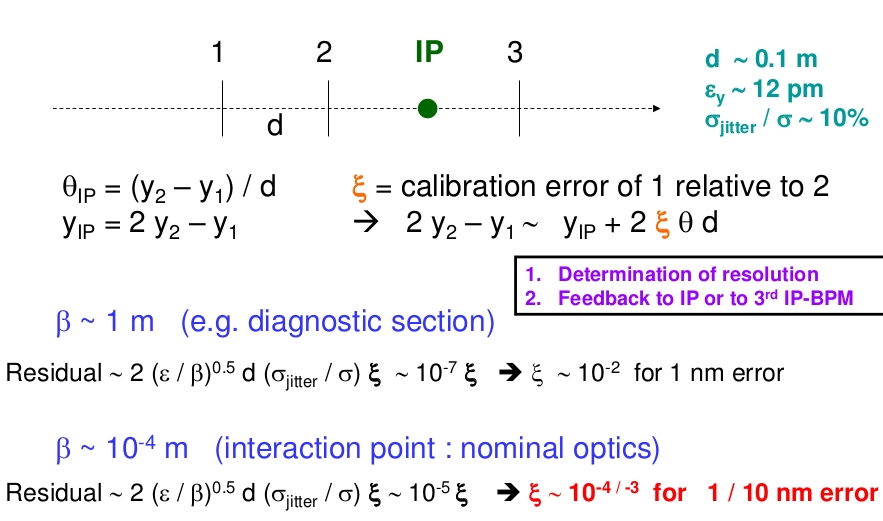
\includegraphics[angle=0,scale=0.35]{scalefactors.jpg}
{\LARGE
  \begin{itemize}
   \item Locate BPMs to enable the \textbf{ maximum possible} beam position resolution
   \item Precision $\sim 5\mu$m
   \item Calibration $\sim 10^{-4}$
  \end{itemize}
 \hspace*{5cm}$\Downarrow$\\
 Displace each BPM block \textbf{independently}
 }\par
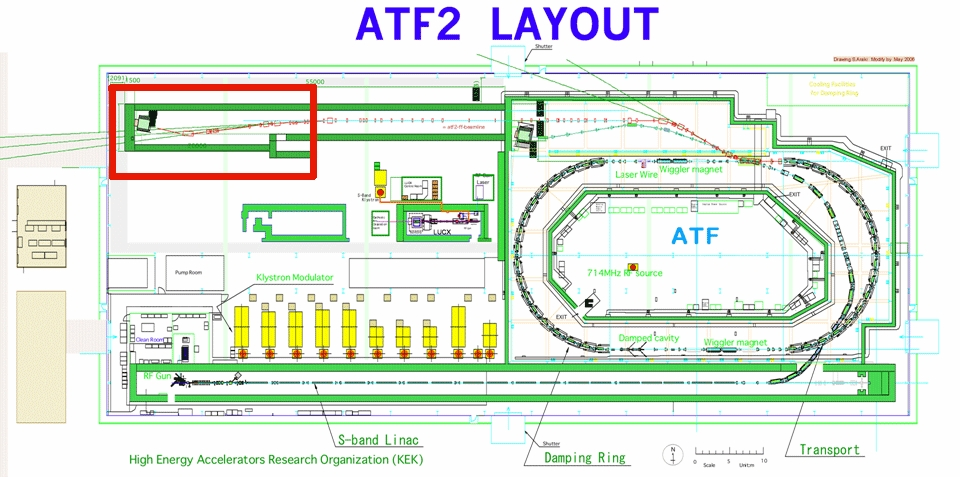
\includegraphics[angle=0,scale=0.2]{ATF2layout33.jpg}
% \end{frame}
% \begin{frame}
\hspace{1cm}
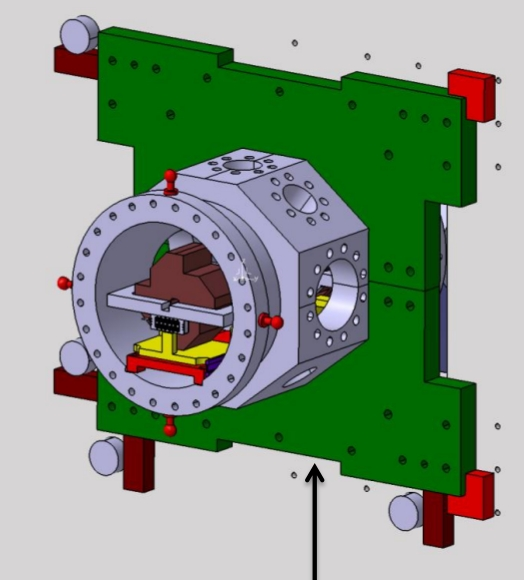
\includegraphics[angle=0,scale=0.16]{chambrevide.jpg}\\
\hspace*{1cm}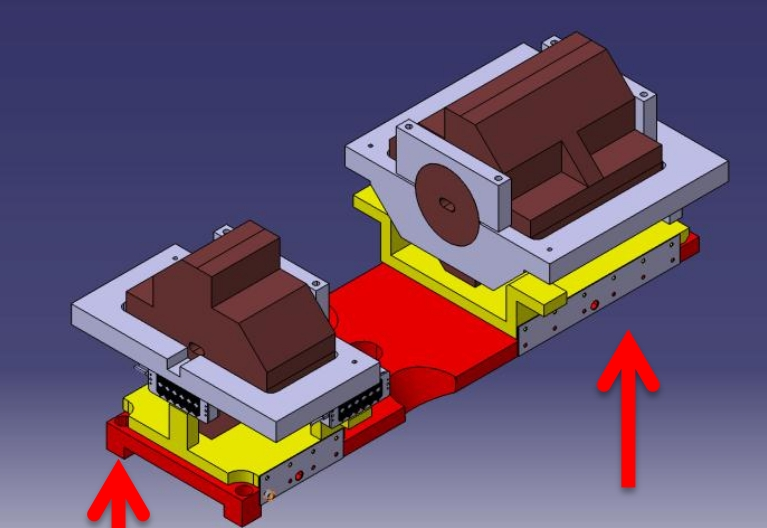
\includegraphics[angle=0,scale=0.22]{BPMs01.jpg}\hspace*{0.2cm}
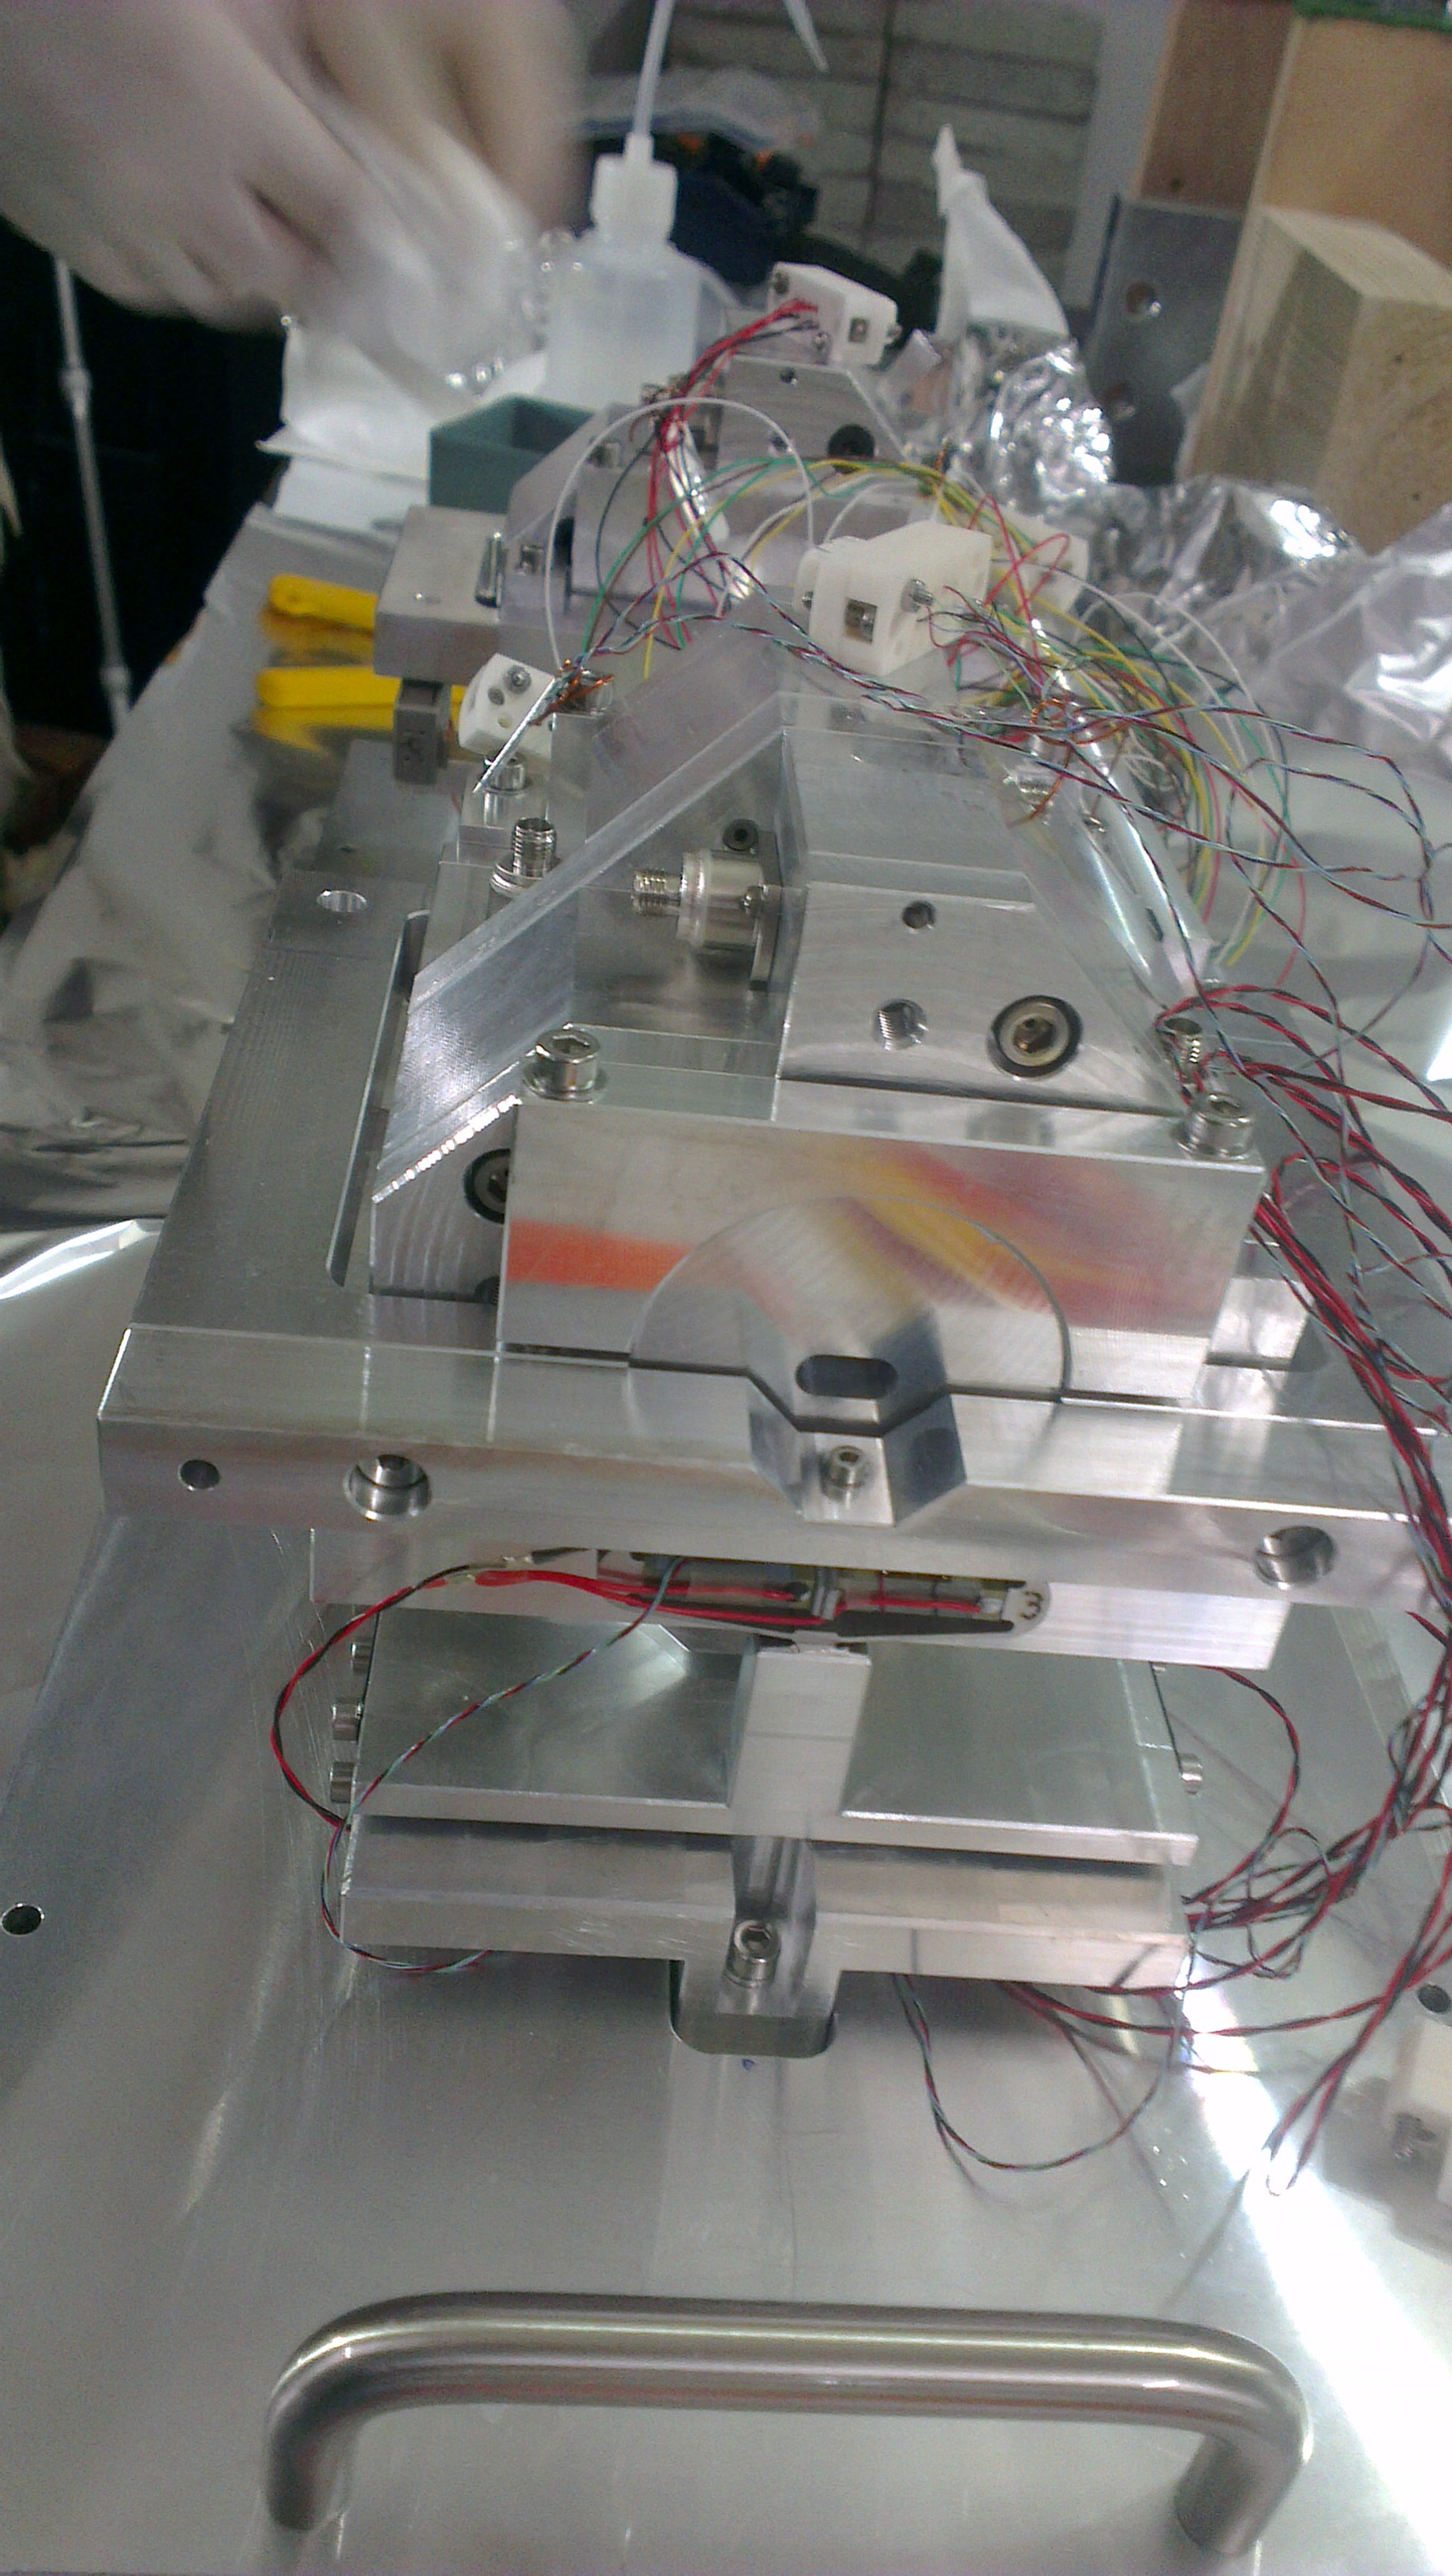
\includegraphics[angle=0,scale=0.0355]{IMAG0460.jpg}\par
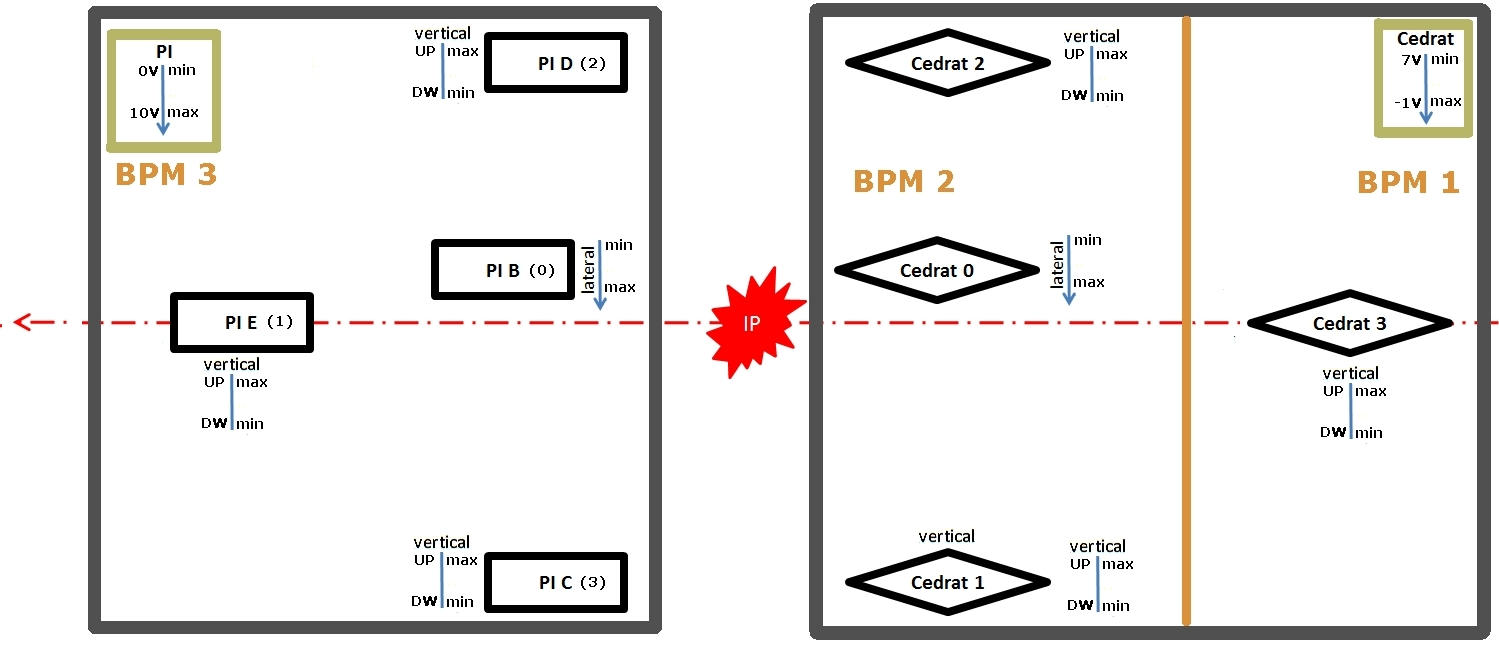
\includegraphics[angle=0,height=7.5cm,width=12cm]{interface.jpg}


\chapter{The System}
\section{System Description}
At the ATF2 IP, inside the vacuum chamber, the BPMs positioning system has been installed during the first two weeks of July 2013.
It will move two blocks:
\begin{itemize}
\item BLOCK BPMs AB
\item BLOCK BPM C
\end{itemize}
This movement has two degrees of freedom: vertical (y) and lateral (x), both transverse to the beam direction. Beam crosses BPMAB first, then and empty space where Shintake monitor laser will be aligned, then crosses BPM3 and goes out of the vacuum chamber.

These two blocks of BPMs, moving in two directions each, are displaced by Piezo-Movers (or just movers) made by different companies. German «PI electronics« moves  BPMC and French «Cedrat Technologies« moves BPMAB.

Each block has 3 vertical and one lateral movers. Lateral is underneath. Four movers are used per block, eight in total.

\section{The Piezo Movers}
Piezo mover changes its position as a function of voltage. Each one of the eight movers has its own control electronics block composed of: 
\begin{itemize}
 \item the mover
\item the strain gauge
\item manufacturer module to:
\begin{itemize}
 \item set piezo mover voltage (high voltage)
 \begin{itemize}
\item PI module E-621
\item CEDRAT module LA75
\end{itemize}
\item read strain gauge
\begin{itemize}
\item PI module E-621 (same as control)
\item CEDRAT module SG75
\end{itemize}
\item set feedback operation (ON/OFF)
\item set control mode (external control from PLC is used)
\end{itemize}
\item PLC channel to
\begin{itemize}
\item set control voltage values equivalent to piezo mover displacement
\item read voltage values equivalent to strain gauge deformation
\end{itemize}
\end{itemize}

\subsection{Mover range}
PI and Cedrat have different ranges: PI (300um), Cedrat (250um)\par

Control voltage and its relation with displacement (min-max) varies between both companies:\par
\begin{itemize}
\item PI: 		(min)   0V   	to 	(max) 10V
\item CEDRAT: 	(max) -1V 	to	(min)    7V
\end{itemize}
It is important to note that:
\begin{itemize}
\item The voltage-displacement relation is inverse for CEDRAT movers.
\item When the system is OFF (0V), PI mover are at its minimum, however CEDRAT are not.
\end{itemize}

\subsection{Feedback and NO Feedback}
There are two operation possibilities per mover: Feedback (fb) and No Feedback (no fb). It means 8 feedback loops. On each case the control module sets a voltage value on the mover and read the strain gauge to create a closed loop. However, their implementations are different on each company.

PI has an analogue feedback system adjusted to the best possible performance on an individual mover (avoid piezo-mover channel interchange). Do not exchange fb/no fb while the equipment is ON. Turn it OFF before any modification. 
Feedback is controlled by the switch number 3  on the front panel. 
Feedback ON (left) / Feedback OFF (right)
During operation, when feedback is ON and working properly two green LED are on (Power LED, On Target LED). When no feedback just the Power LED is green.

Cedrat has a digital feedback system with PID parameters per mover. Avoid piezo-mover channel interchange. Feedback could be turn off/on by two means:
Switch SERVO ON in the front pannel. Feedback ON(right)/Feedback OFF (left)
Using sofware  HDPM45V16. To activate or desactivate permanently the fb.

\section{The PLC}
Two NI9263 are used to set analogue voltage into the mover control electronics.\par
Two NI9239 are used to read analogue voltage from the strain gauge readback.\par
One NI9219 is used to read temperature.\par
These modules are connected to the chassis NI9188 which is connected by network to a working station with Labview installed.
The block chassis+NI modules is called \textbf{PLC}.\par

National instruments Chassis: NI9188
\begin{itemize}
\item Mac Address: 0080.2f14.b777
\item DHCP
\item IP address (ATF) 31.1.1.39
\item IP address (KEK): None
\item Host name: ipmv-plc.ip-local
\item Net Mask: 255.255.255.0
\item connected to ip-local during installation
\item Chassis NI9188 can connect up to 8 modules, not all are used:
\begin{itemize}
\item PI
\begin{itemize}
\item Module 5: NI9263 Digital to analogue converter
\item Module 6: NI9239 Analogue to digital converter
\end{itemize}
\item Cedrat
\begin{itemize}
\item Module 2: NI9263 Digital to analogue converter
\item Module 3: NI9239 Analogue to digital converter
\end{itemize}
\item Temperature
\begin{itemize}
\item Module 8: NI9219 Temperature probes
\begin{itemize}
\item Cedrat: 	Channel 0
\item PI: Channel 2
\end{itemize}
\end{itemize}
\end{itemize}
\end{itemize}

\section{The PC}
It is used to control from close locations the BPM positioning system. It sets the digital values to put in the PLC and reads the digital values from the PLC channels corresponding to strain gauges.\par

\subsection{Used Software}
Windows 7 Français\par
National Instrument - Labview 2011\par
National Instruments - Measurement $\&$s Automation Explorer (NI MAX)\par
Gimp 2.8\par
Microsoft office – Excel 2013\par
cmd\par
Highly Dynamic and Precise motion 45 V 1.6 (HDPM45V16)– Cedrat Technologies\par
LAL Computer (Laptop)\par
Account: **********(not in this document)\par
Password: *********(not in this document)\par
Processor Inter Core i7 vPro\par
Mac Address: d067.e550.620e\par
DHCP\par
IP address(ATF): 31.1.1.38\par
IP address (KEK): Wifi connection (MAC registered at KEK)\par
Net Mask: 255.255.255.0\par
connected to ip-local during installation\par
Folder Content description\par
Path to applications and info\par
Bureau/Actionneurs Piezo/Applis\par
All applications were done in Labview. Title gives a hint of its content:\par
	(keywords used in titles):
oscilloscope: uses de ADC to read signals\par
generateur: function generator, uses de DACs to produce signals\par
Actionneurs positionnement BPMs: activate the system displacement\par
Ethernet: connected by wired network,\par
USB: corresponds to previous version connected by USB.\par
Verticaux groupe: all 3 vertical mover movers are activated by one voltage control\par
 mouvements identiques: first version of BPM displacement system (PI and CEDRAT) integrated.\par
Jauges: stores the strain gauges info in excel format.\par
temp: stores temperature info in excel format.\par
epics: control from epics system, Labview works as interface.\par
Actionneurs multicycles: several cycles over the defined voltage range are performed\par
Cedrat, PI: identifies the group of movers to use.\par
Vertical, lateral fixe: it means that one direction of movement is set (fixed) to a voltage value while the other direction varies in cycles.\par

\section{The BPMs}
\subsection{Coordinate system}\par
\centering
Each BPM has its own coordinates with respect to a reference system centered \textbf{electrically} and aligned with the beam
%\begin{columns}[t]
%\begin{column}{3.5cm}
  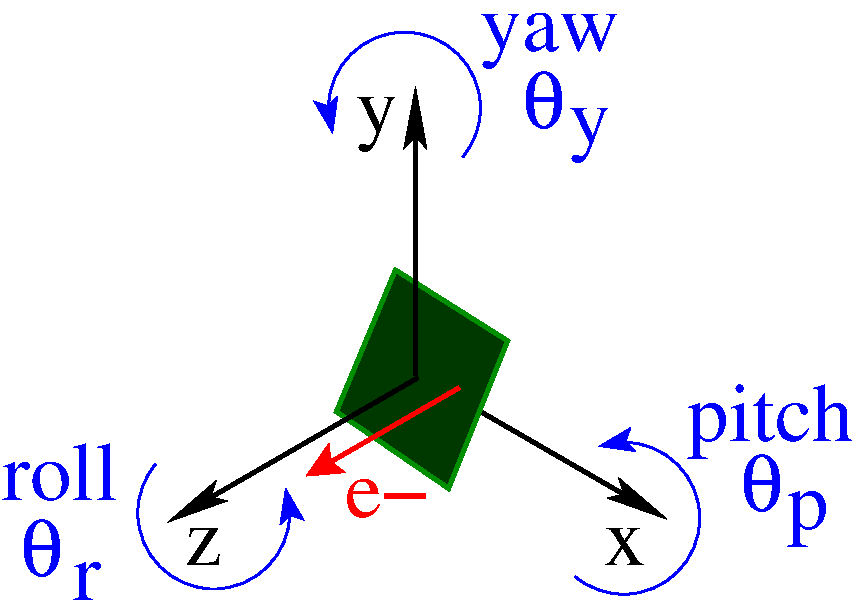
\includegraphics[scale=0.3,angle=0]{fig23.pdf}\\
  {\color{red}Beam}, {\color{forestgreen} BPMs}\\
%\end{column}
%\begin{column}{7cm}
\vspace{-3.3cm}
% \textbf{Variables}
\begin{itemize}
 \item Beam Position
 \\$x_A,y_A,z_A$\\$x_B,y_B,z_B$\\$x_C,y_C,z_C$
 \item BPM Angles respect to ref. system\\
 $\theta_{Ap},\theta_{Ar},\theta_{Ay}$\\
 $\theta_{Bp},\theta_{Br},\theta_{By}$\\
 $\theta_{Cp},\theta_{Cr},\theta_{Cy}$
\end{itemize}
%\end{column}
%\end{columns}
\centering
{\tiny All systems relate to a common \textbf{mechanical} reference system, no rotations, just translations}\\
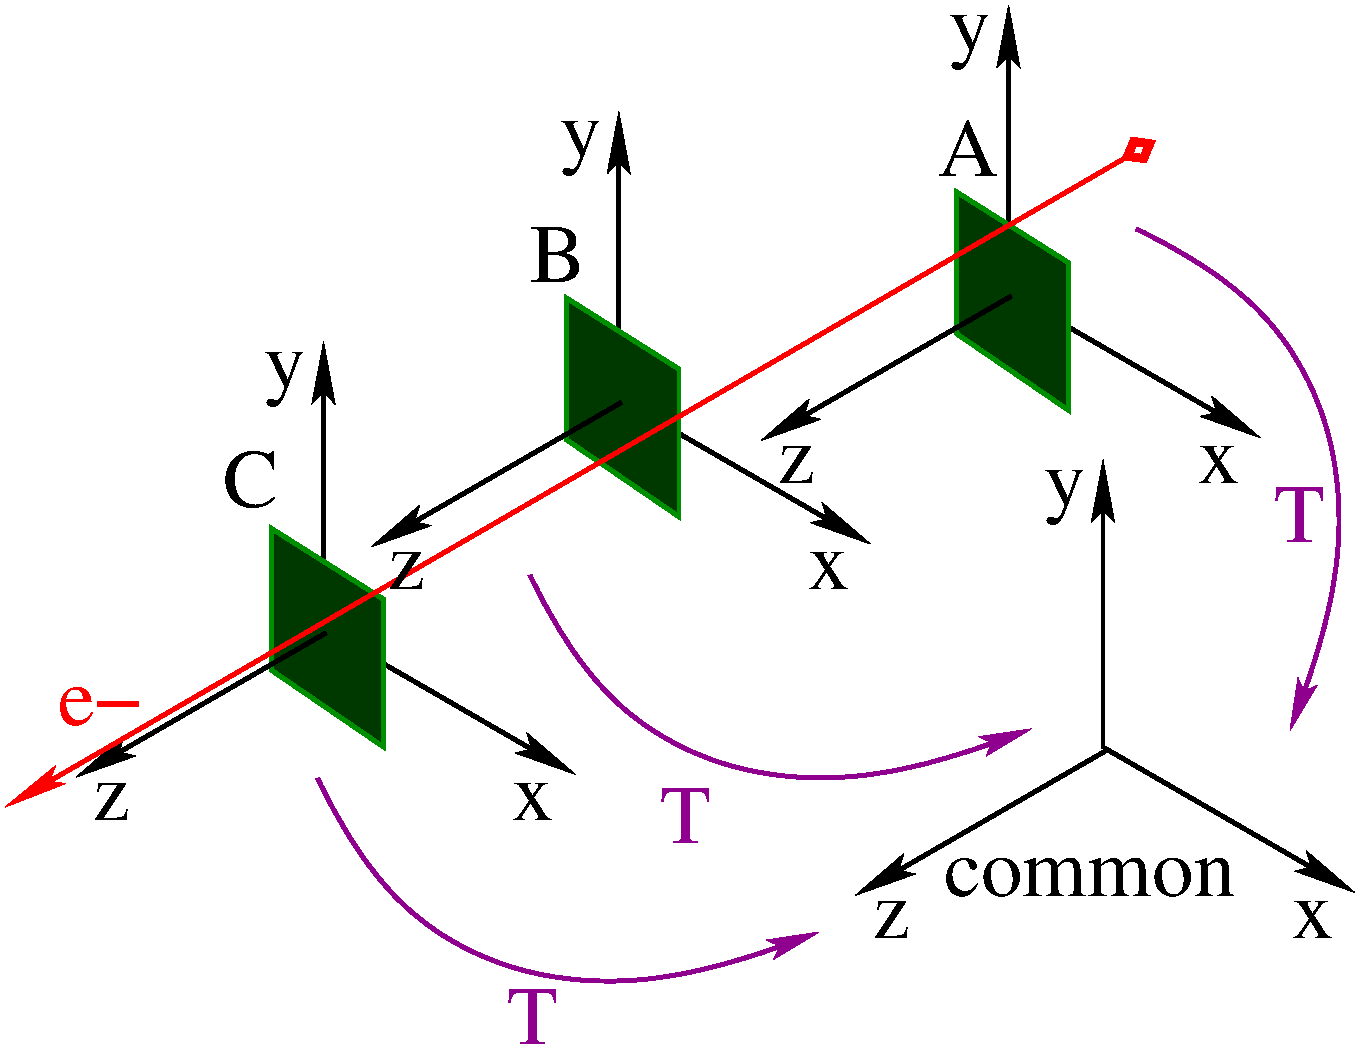
\includegraphics[scale=0.2,angle=0]{fig17.pdf}\\\centering
{\tiny \textbf{One of the BPMs reference system could be chosen to coincide with the common}\\
% \\Ideally just translations in the longitudinal direction
}
% \\

%\begin{frame}{Movers}\centering
{\tiny There is a set of movers to control BPM position}\vspace{-0.5cm}
\centering
%\begin{columns}
%\begin{column}{3.5cm}
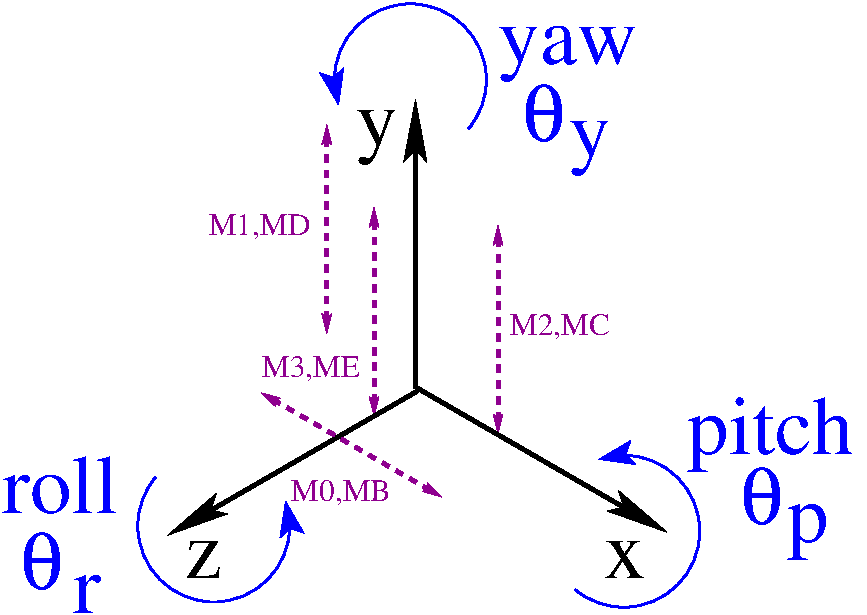
\includegraphics[scale=0.30,angle=0]{fig25.pdf} 
%\end{column}
%\begin{column}{5.5cm}
\begin{align*}
 x &= x_0+f_x(M_{0,B})\\
 y &= y_0+f_y(M_{123,CDE})\\
 z &= z_0\\
 \theta_p &= \theta_{p0}+f_p(M_{123,CDE})\\
 \theta_r &= \theta_{r0}\\
 \theta_y &= \theta_{y0}
\end{align*}\par
\vspace*{-0.4cm}{\tiny All initial values are set during the IP BPMs installation}
%\end{column}
%\end{columns}\vspace*{0.5cm}
%\begin{columns}
% \begin{column}{5cm}
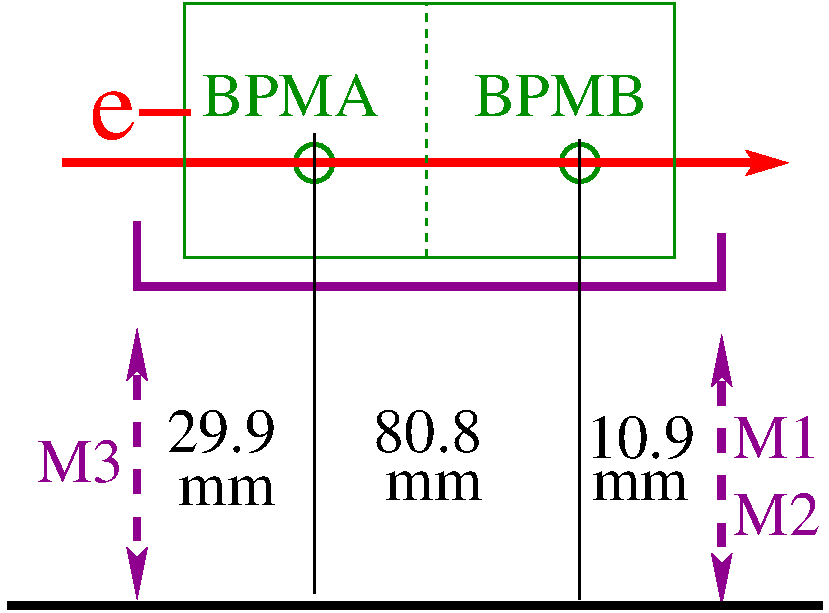
\includegraphics[scale=0.25,angle=0]{fig27.pdf}
% \end{column}
%\begin{column}{5cm}
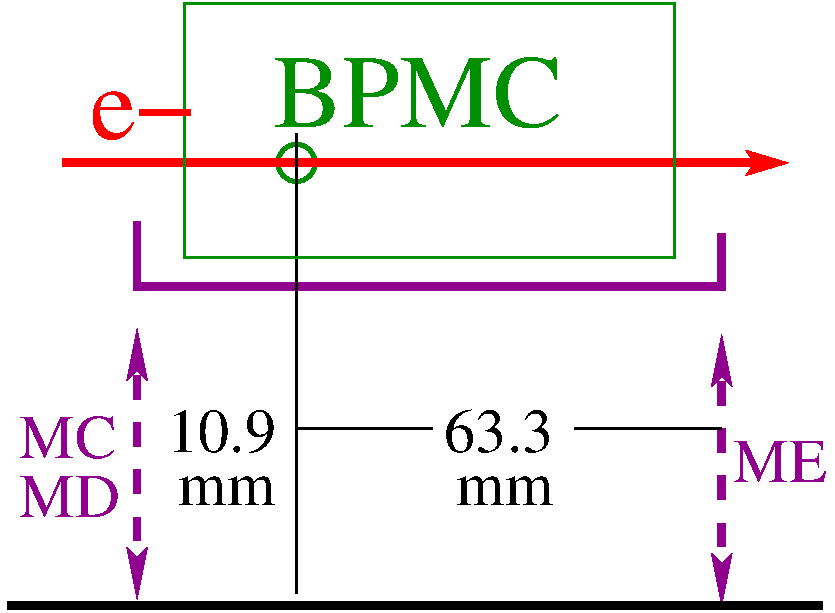
\includegraphics[scale=0.25,angle=0]{fig26.pdf}
% \end{column}
%\end{columns}
% \end{frame}


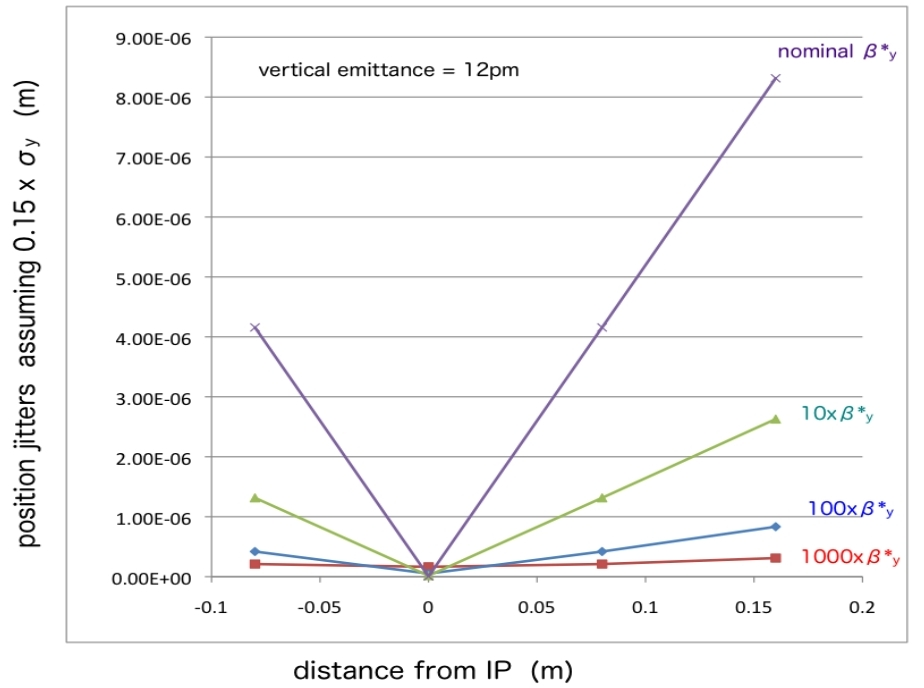
\includegraphics[scale=0.3,angle=0]{pos_beta2}

\subsection{Sensitivity to angle (BPMA)}
$1000\beta_y$ optics. 51 bunches recorded per each mover position. Maximum IQ value was picked each time.\\
\centering
 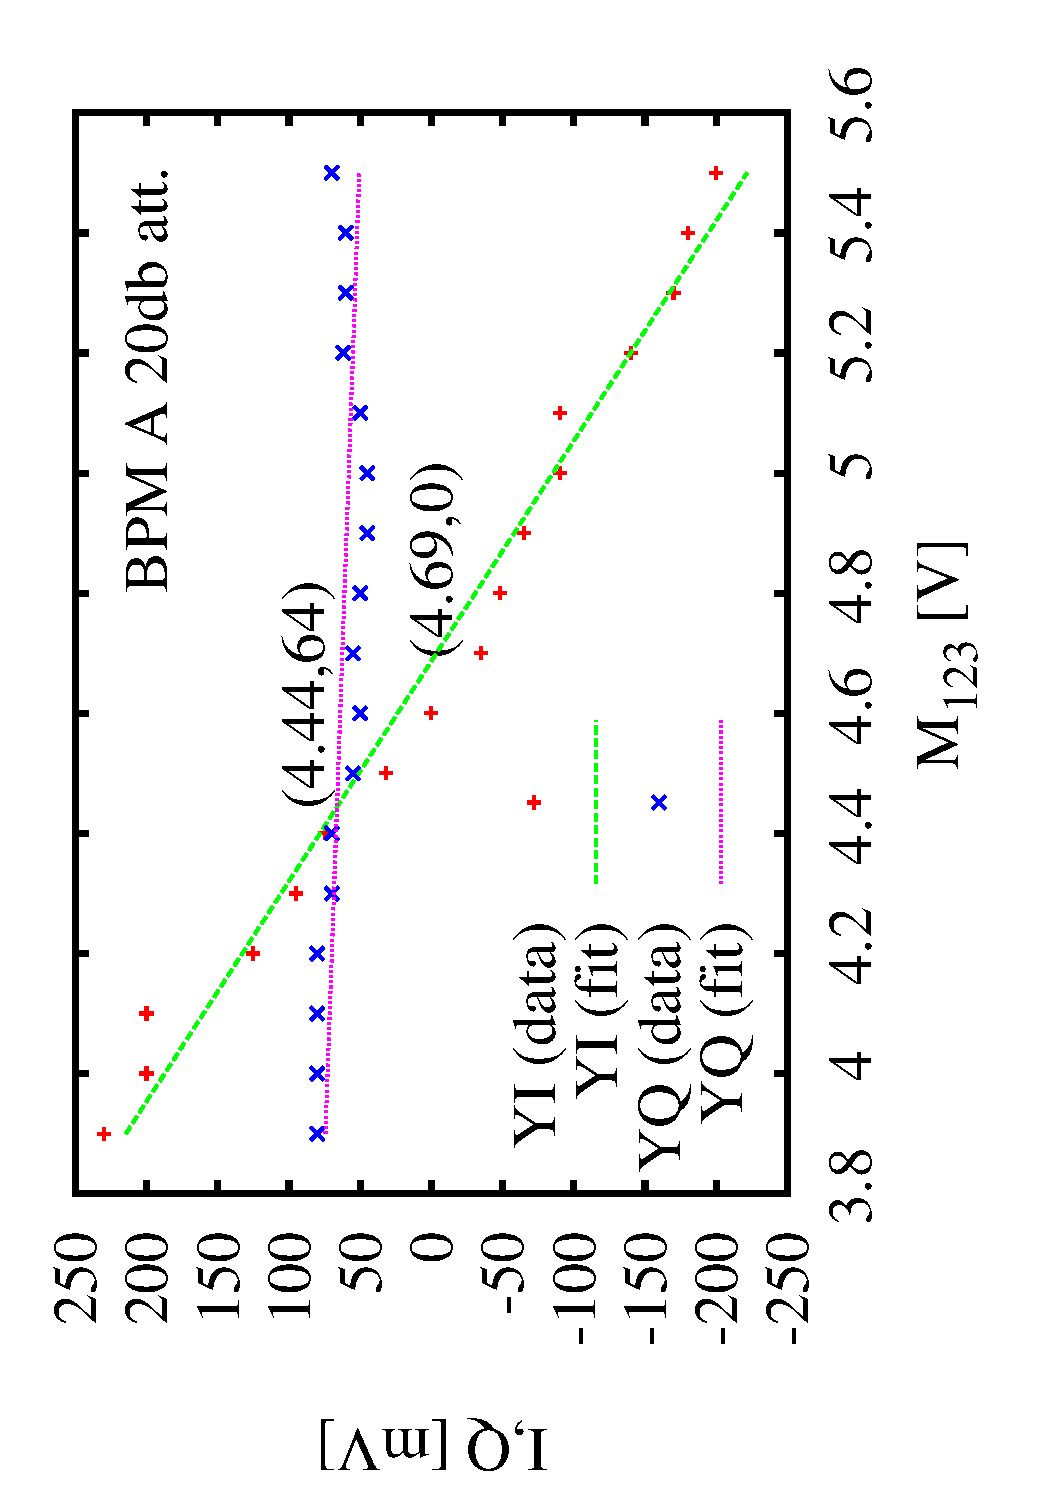
\includegraphics[scale=0.3,angle=-90]{image01_sense.pdf}\\
 \begin{equation}
  (4.69[\text{V}]-4.44[\text{V}])\left(\frac{250[\mu\text{m}]}{8[\text{V}]}\right)\left(\frac{1}{1.6[\text{mrad}]}\right)=4.9\left[\frac{\mu\textmd{m}}{\textmd{mrad}}\right]
 \end{equation}
\raggedright

\section{Electrical connections}
\hspace*{1.4cm}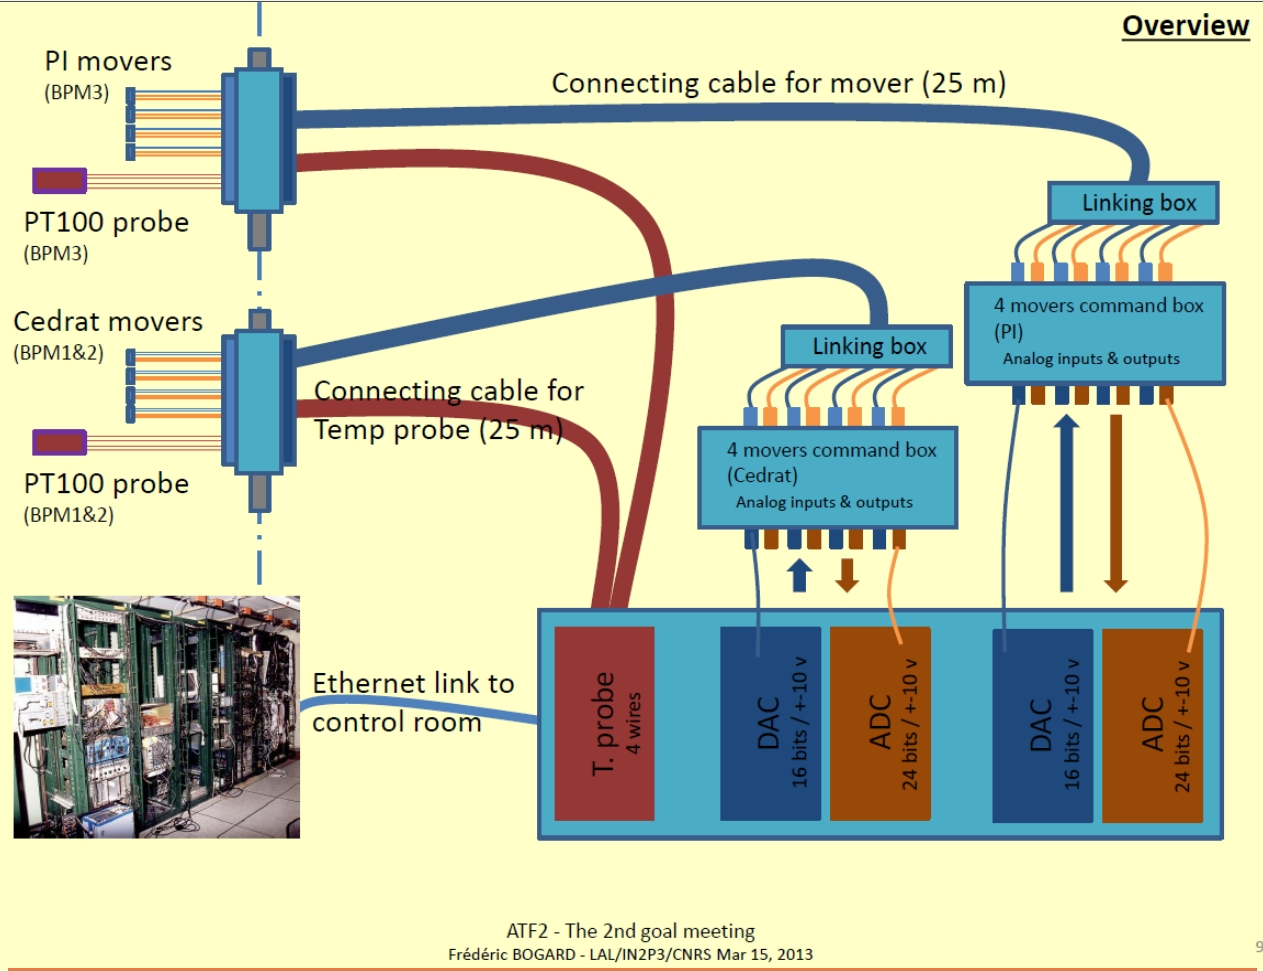
\includegraphics[angle=0,scale=0.2]{link.jpg}\par
%\hspace*{1.4cm}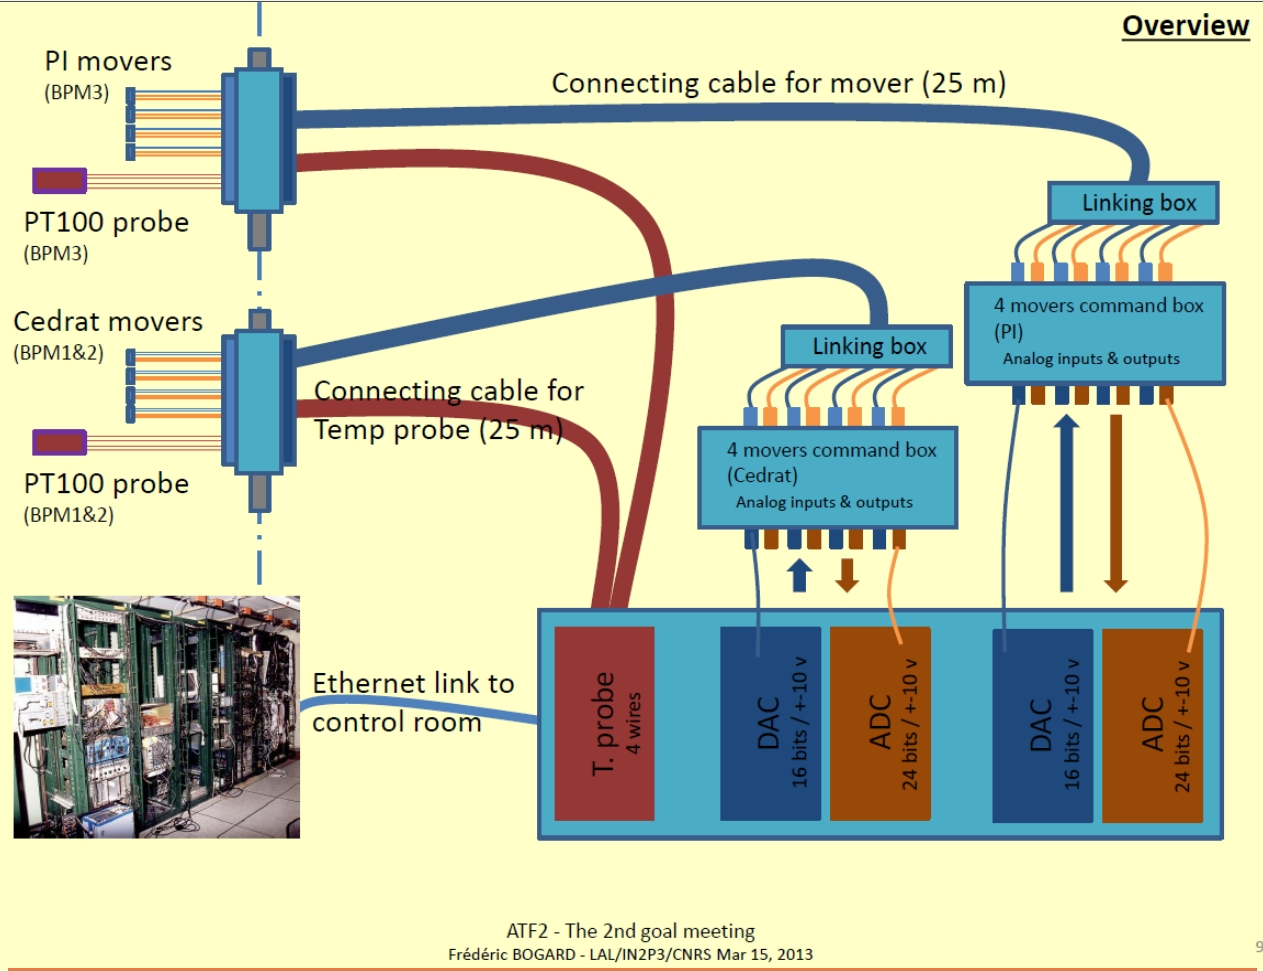
\includegraphics[angle=0,scale=0.2]{link.jpg}
\begin{tikzpicture}
  \node (img1) {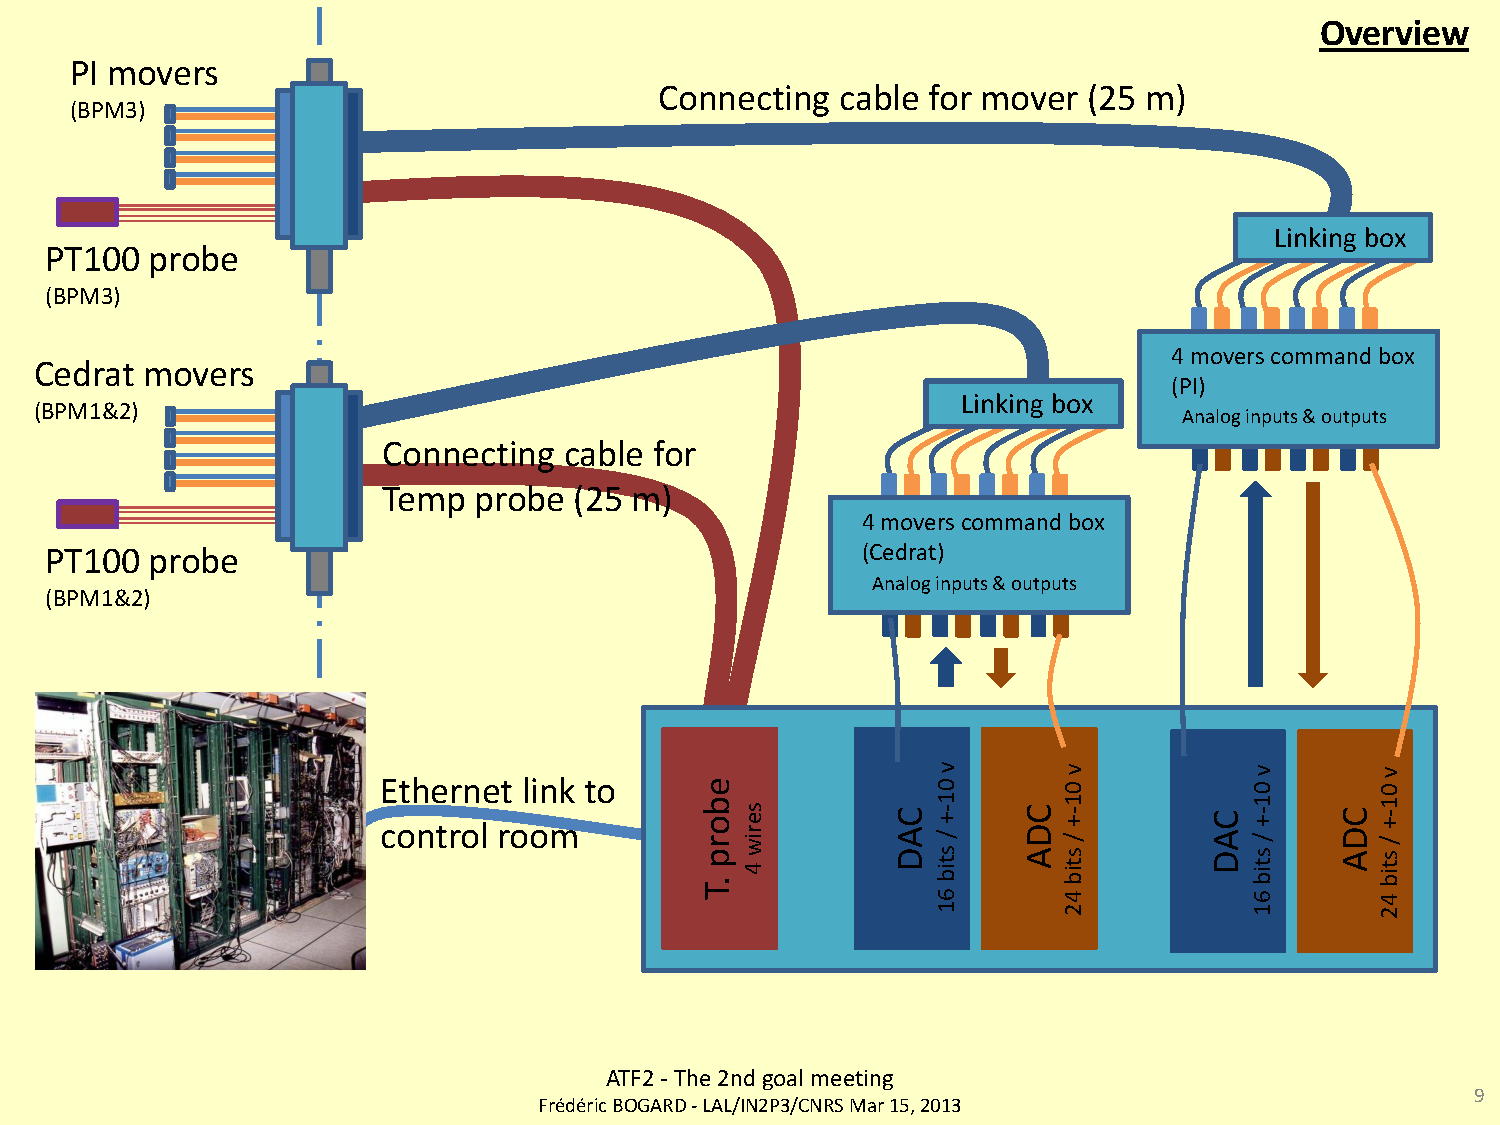
\includegraphics[scale=0.45,angle=0]{elect01.pdf}};
 %\pause
  \node (img2) at (-4.2,-3) {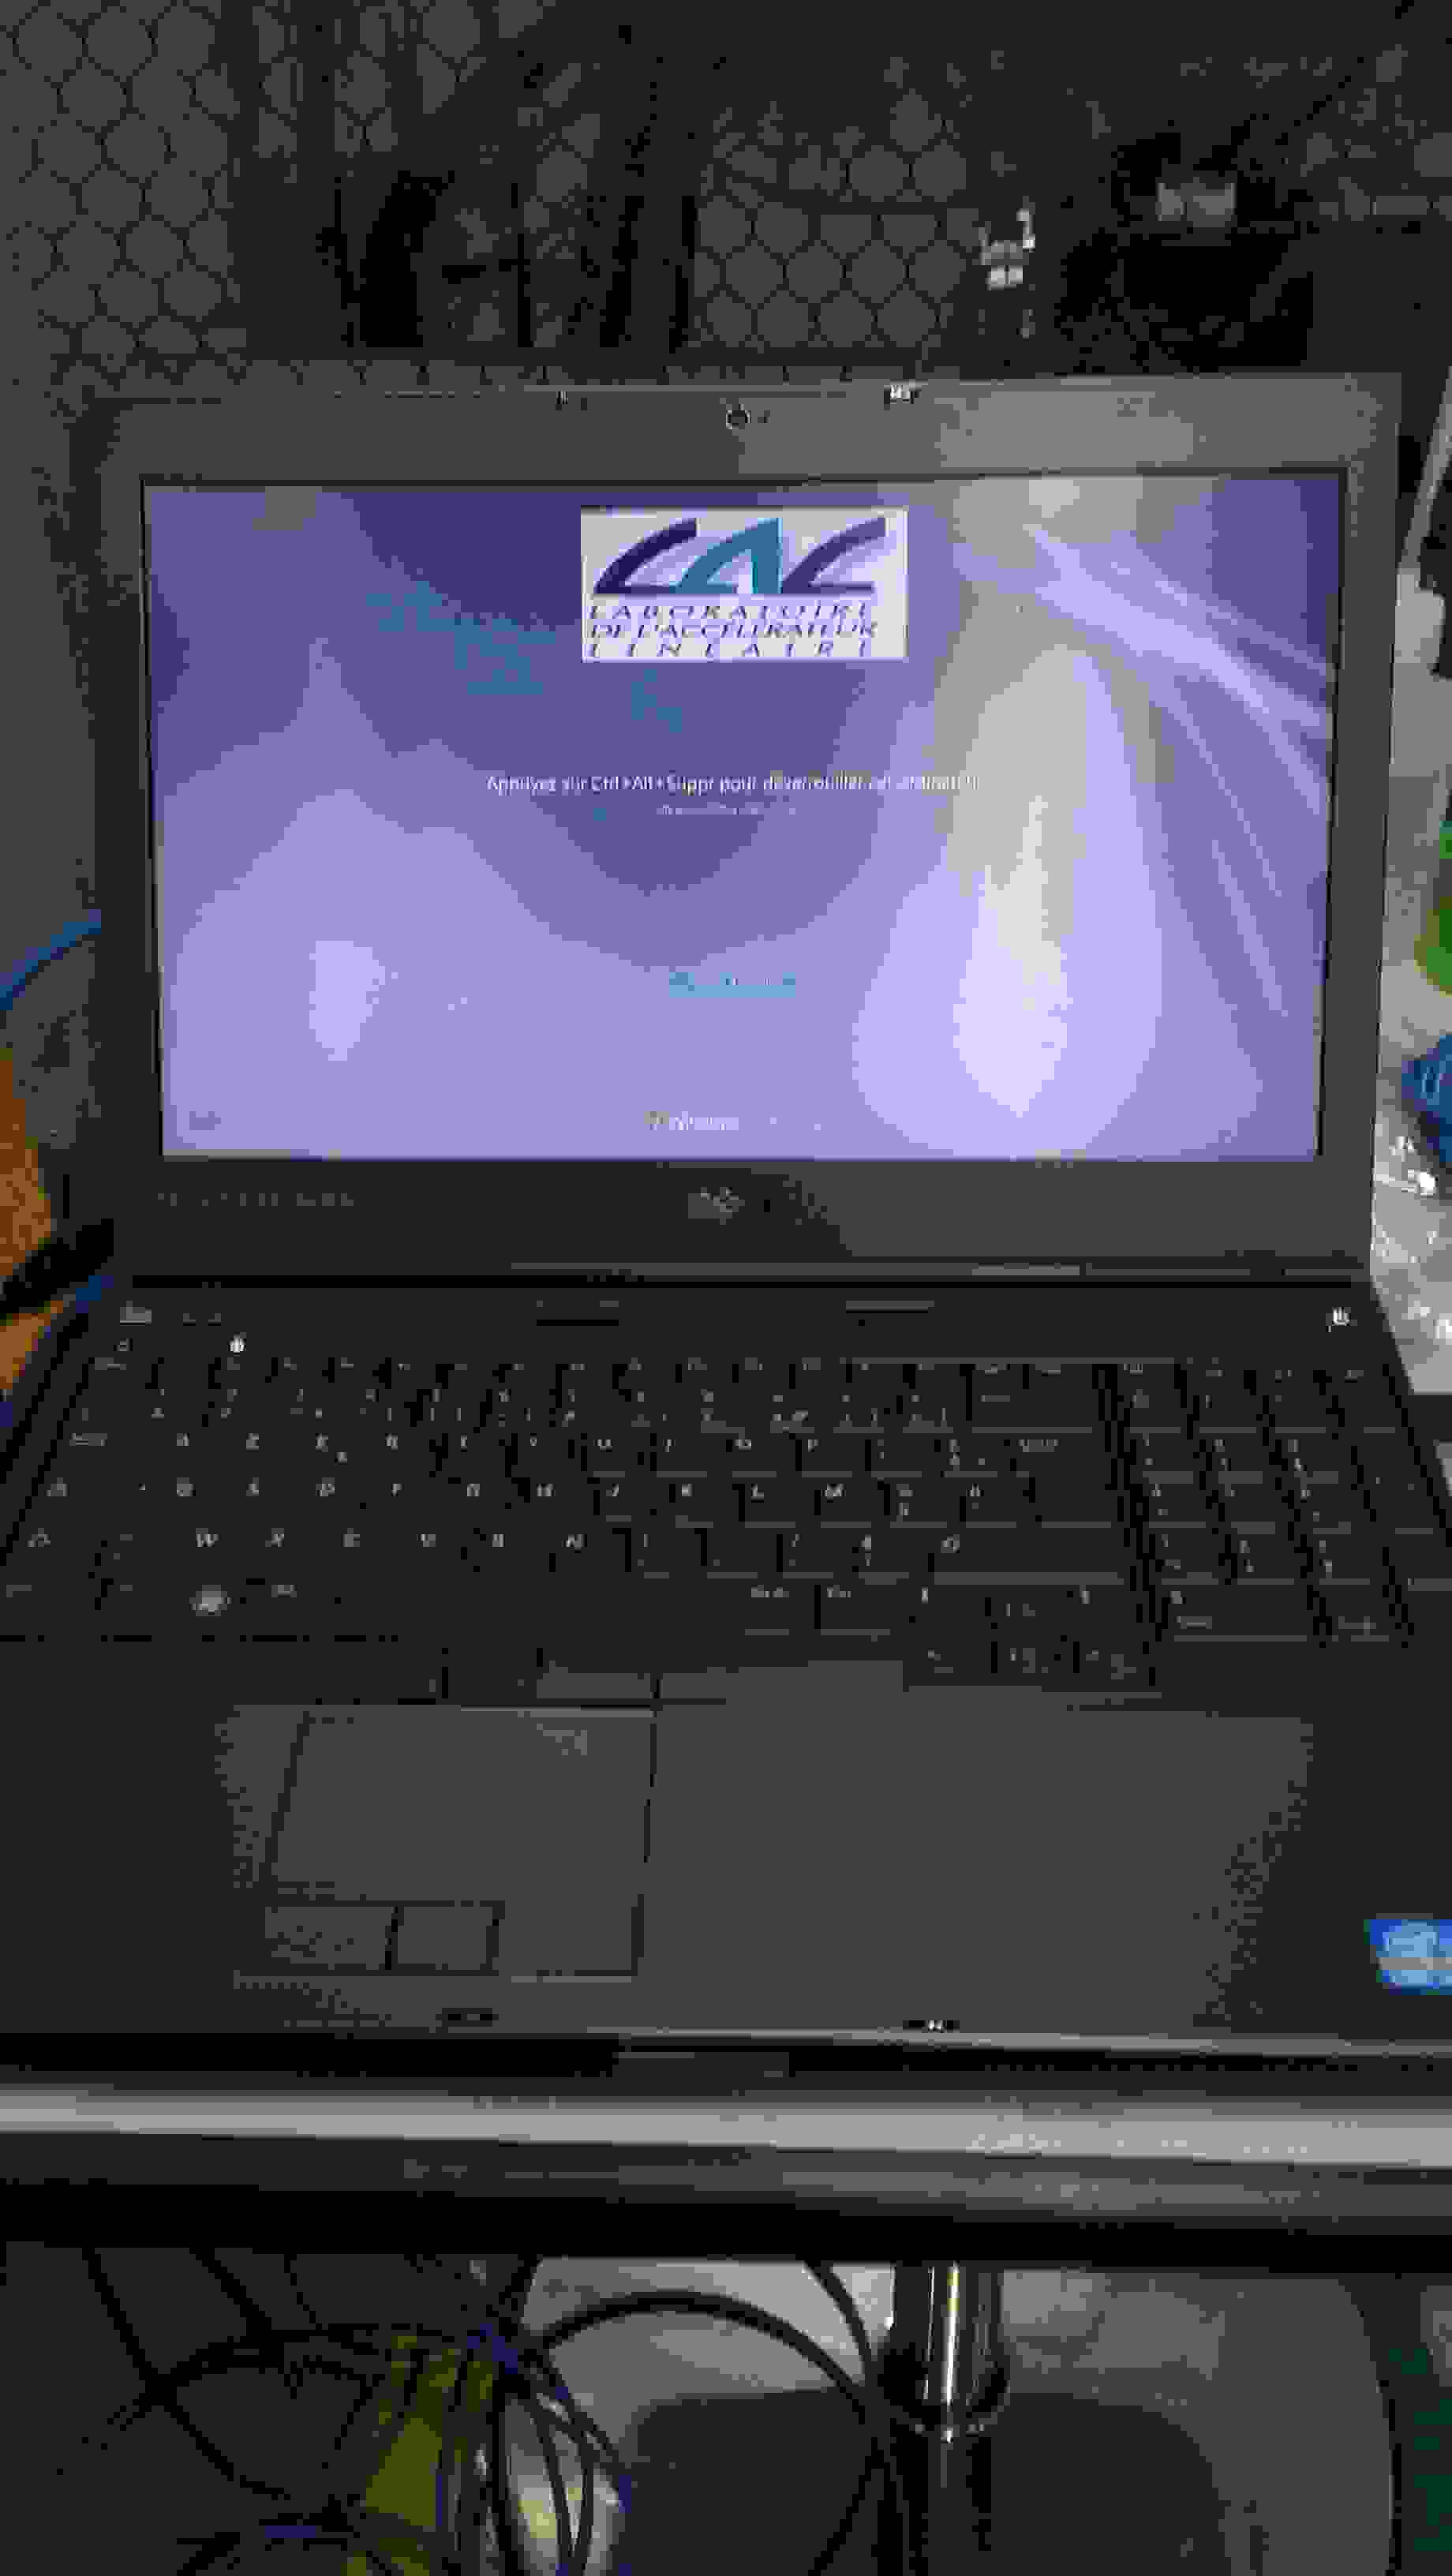
\includegraphics[scale=0.039,angle=0]{ima02a.jpg}};
%   \pause
  \node (img3) at (2.2,-2.1) {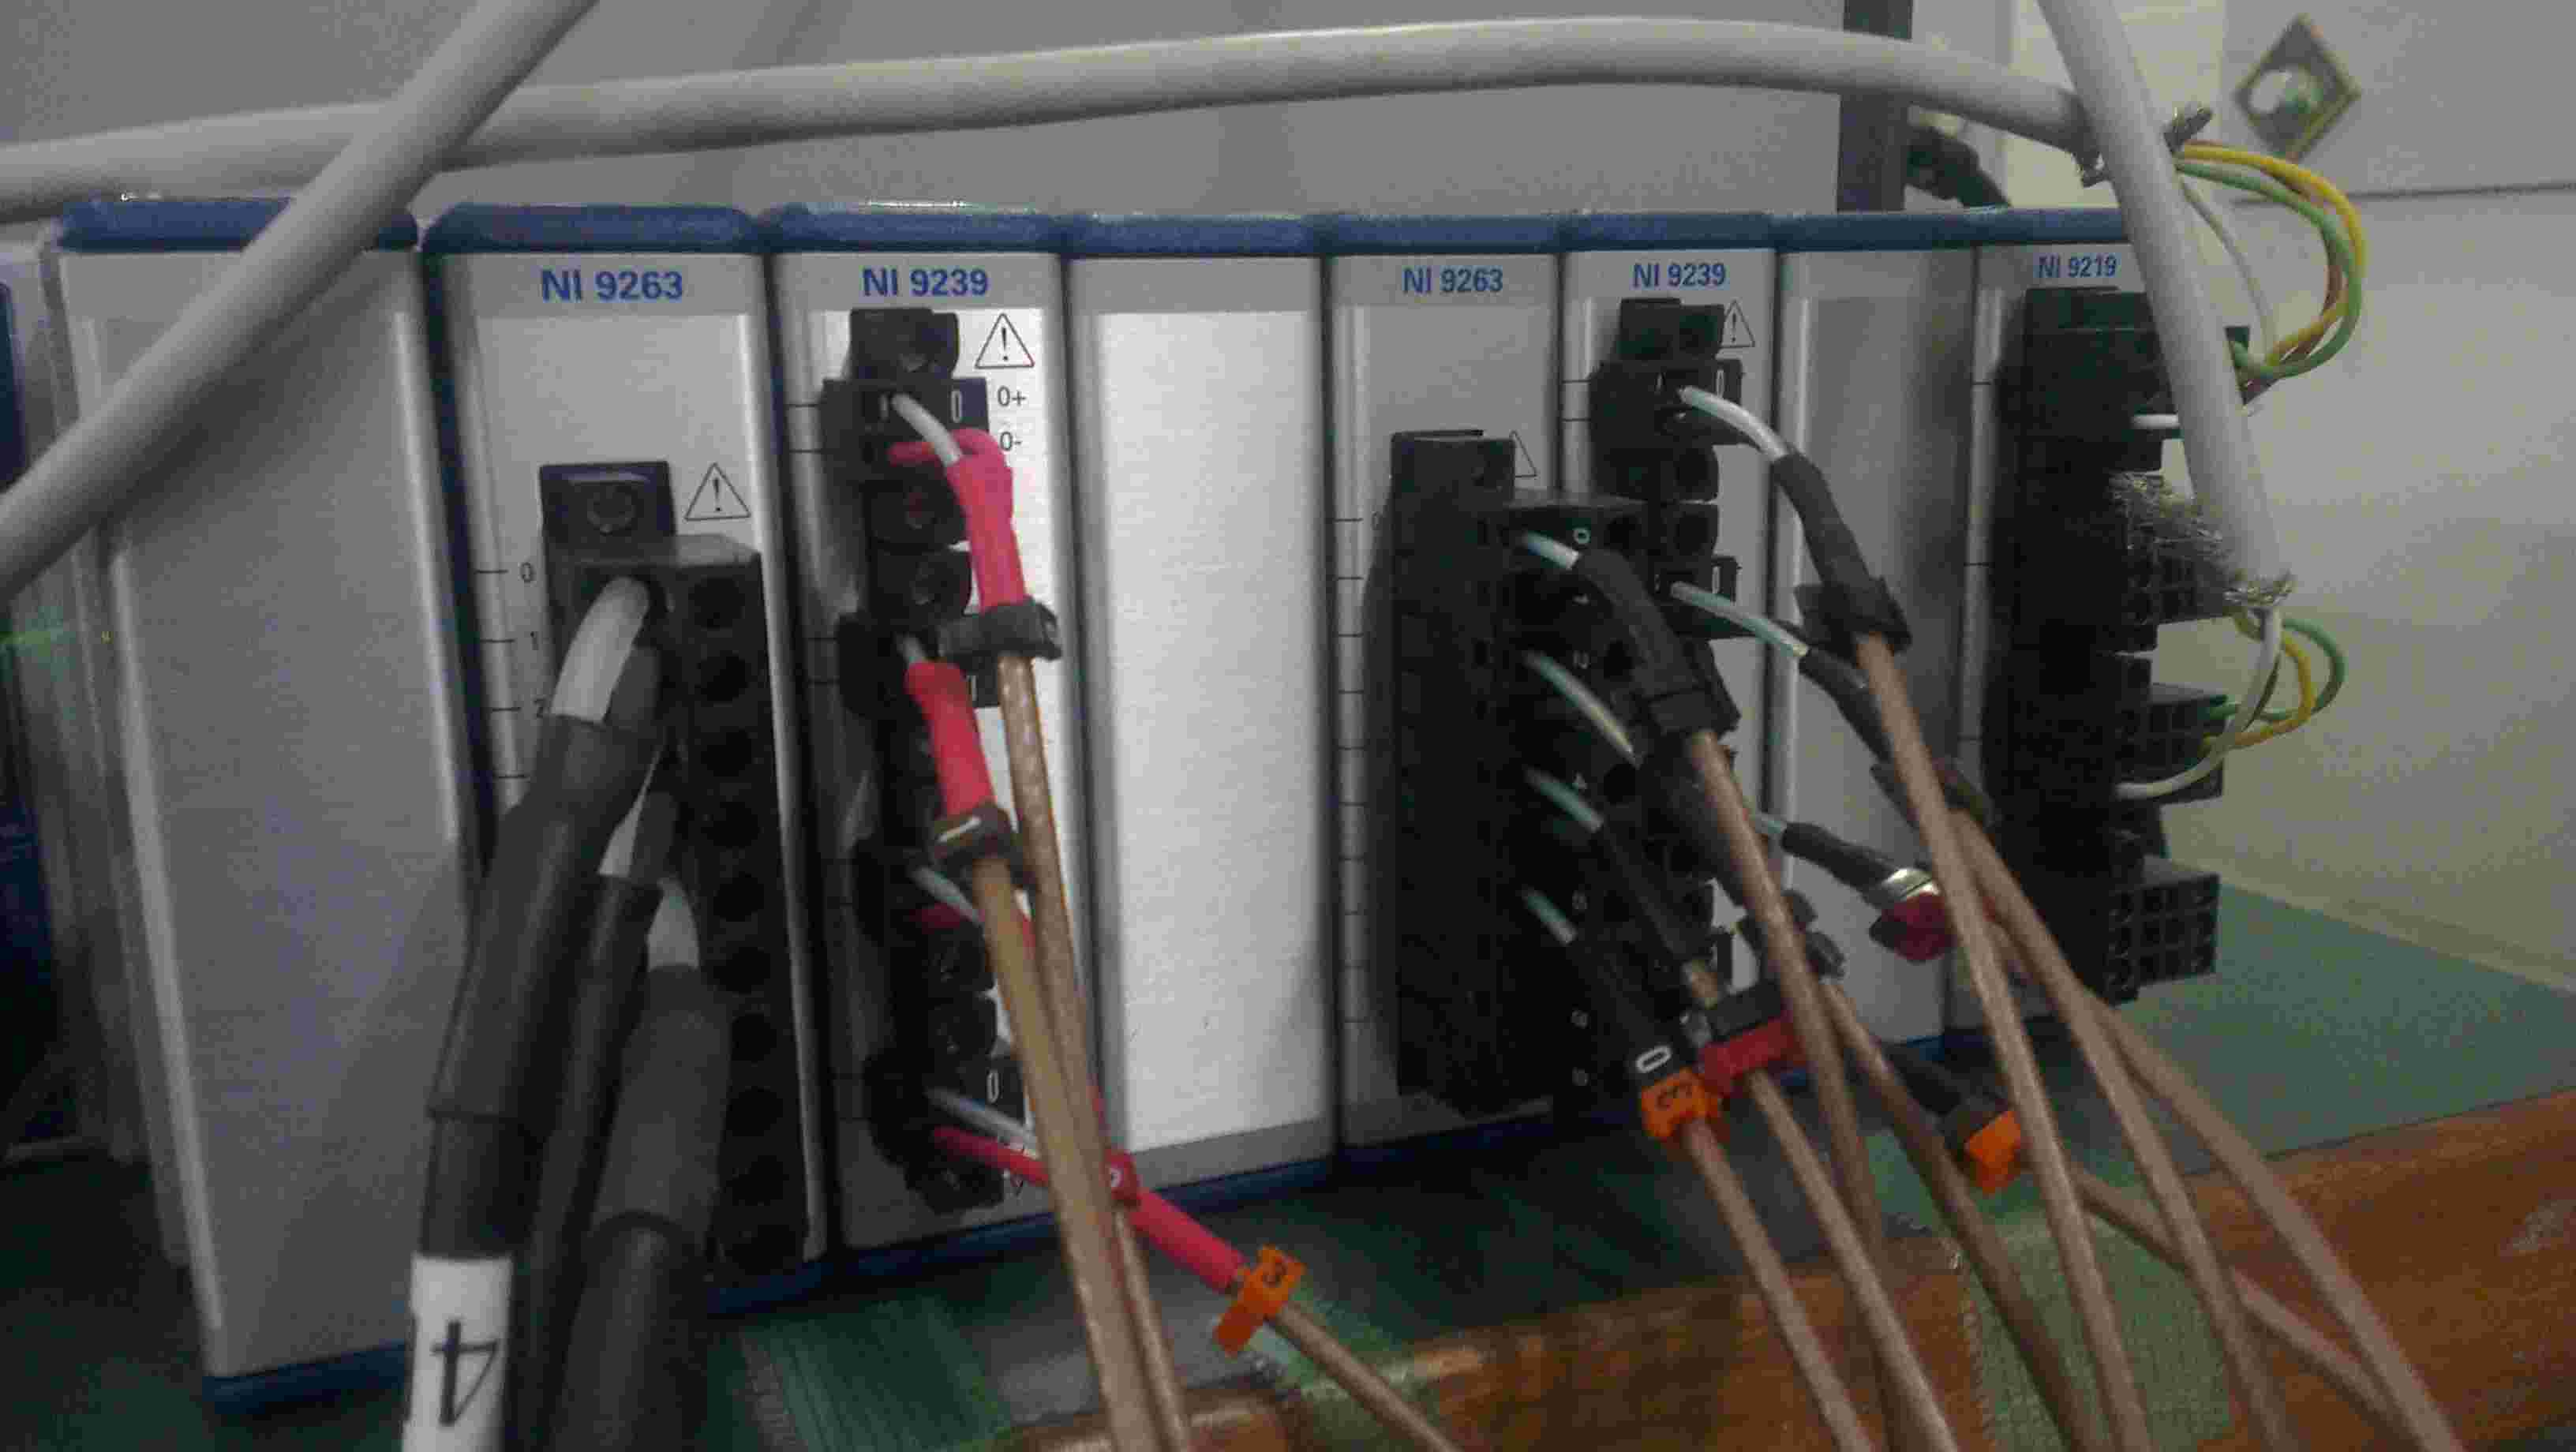
\includegraphics[height=2.5cm,width=6.2cm,angle=180]{ima06a.jpg}};
%   \pause
  \node (img4) at (4.4,1.0) {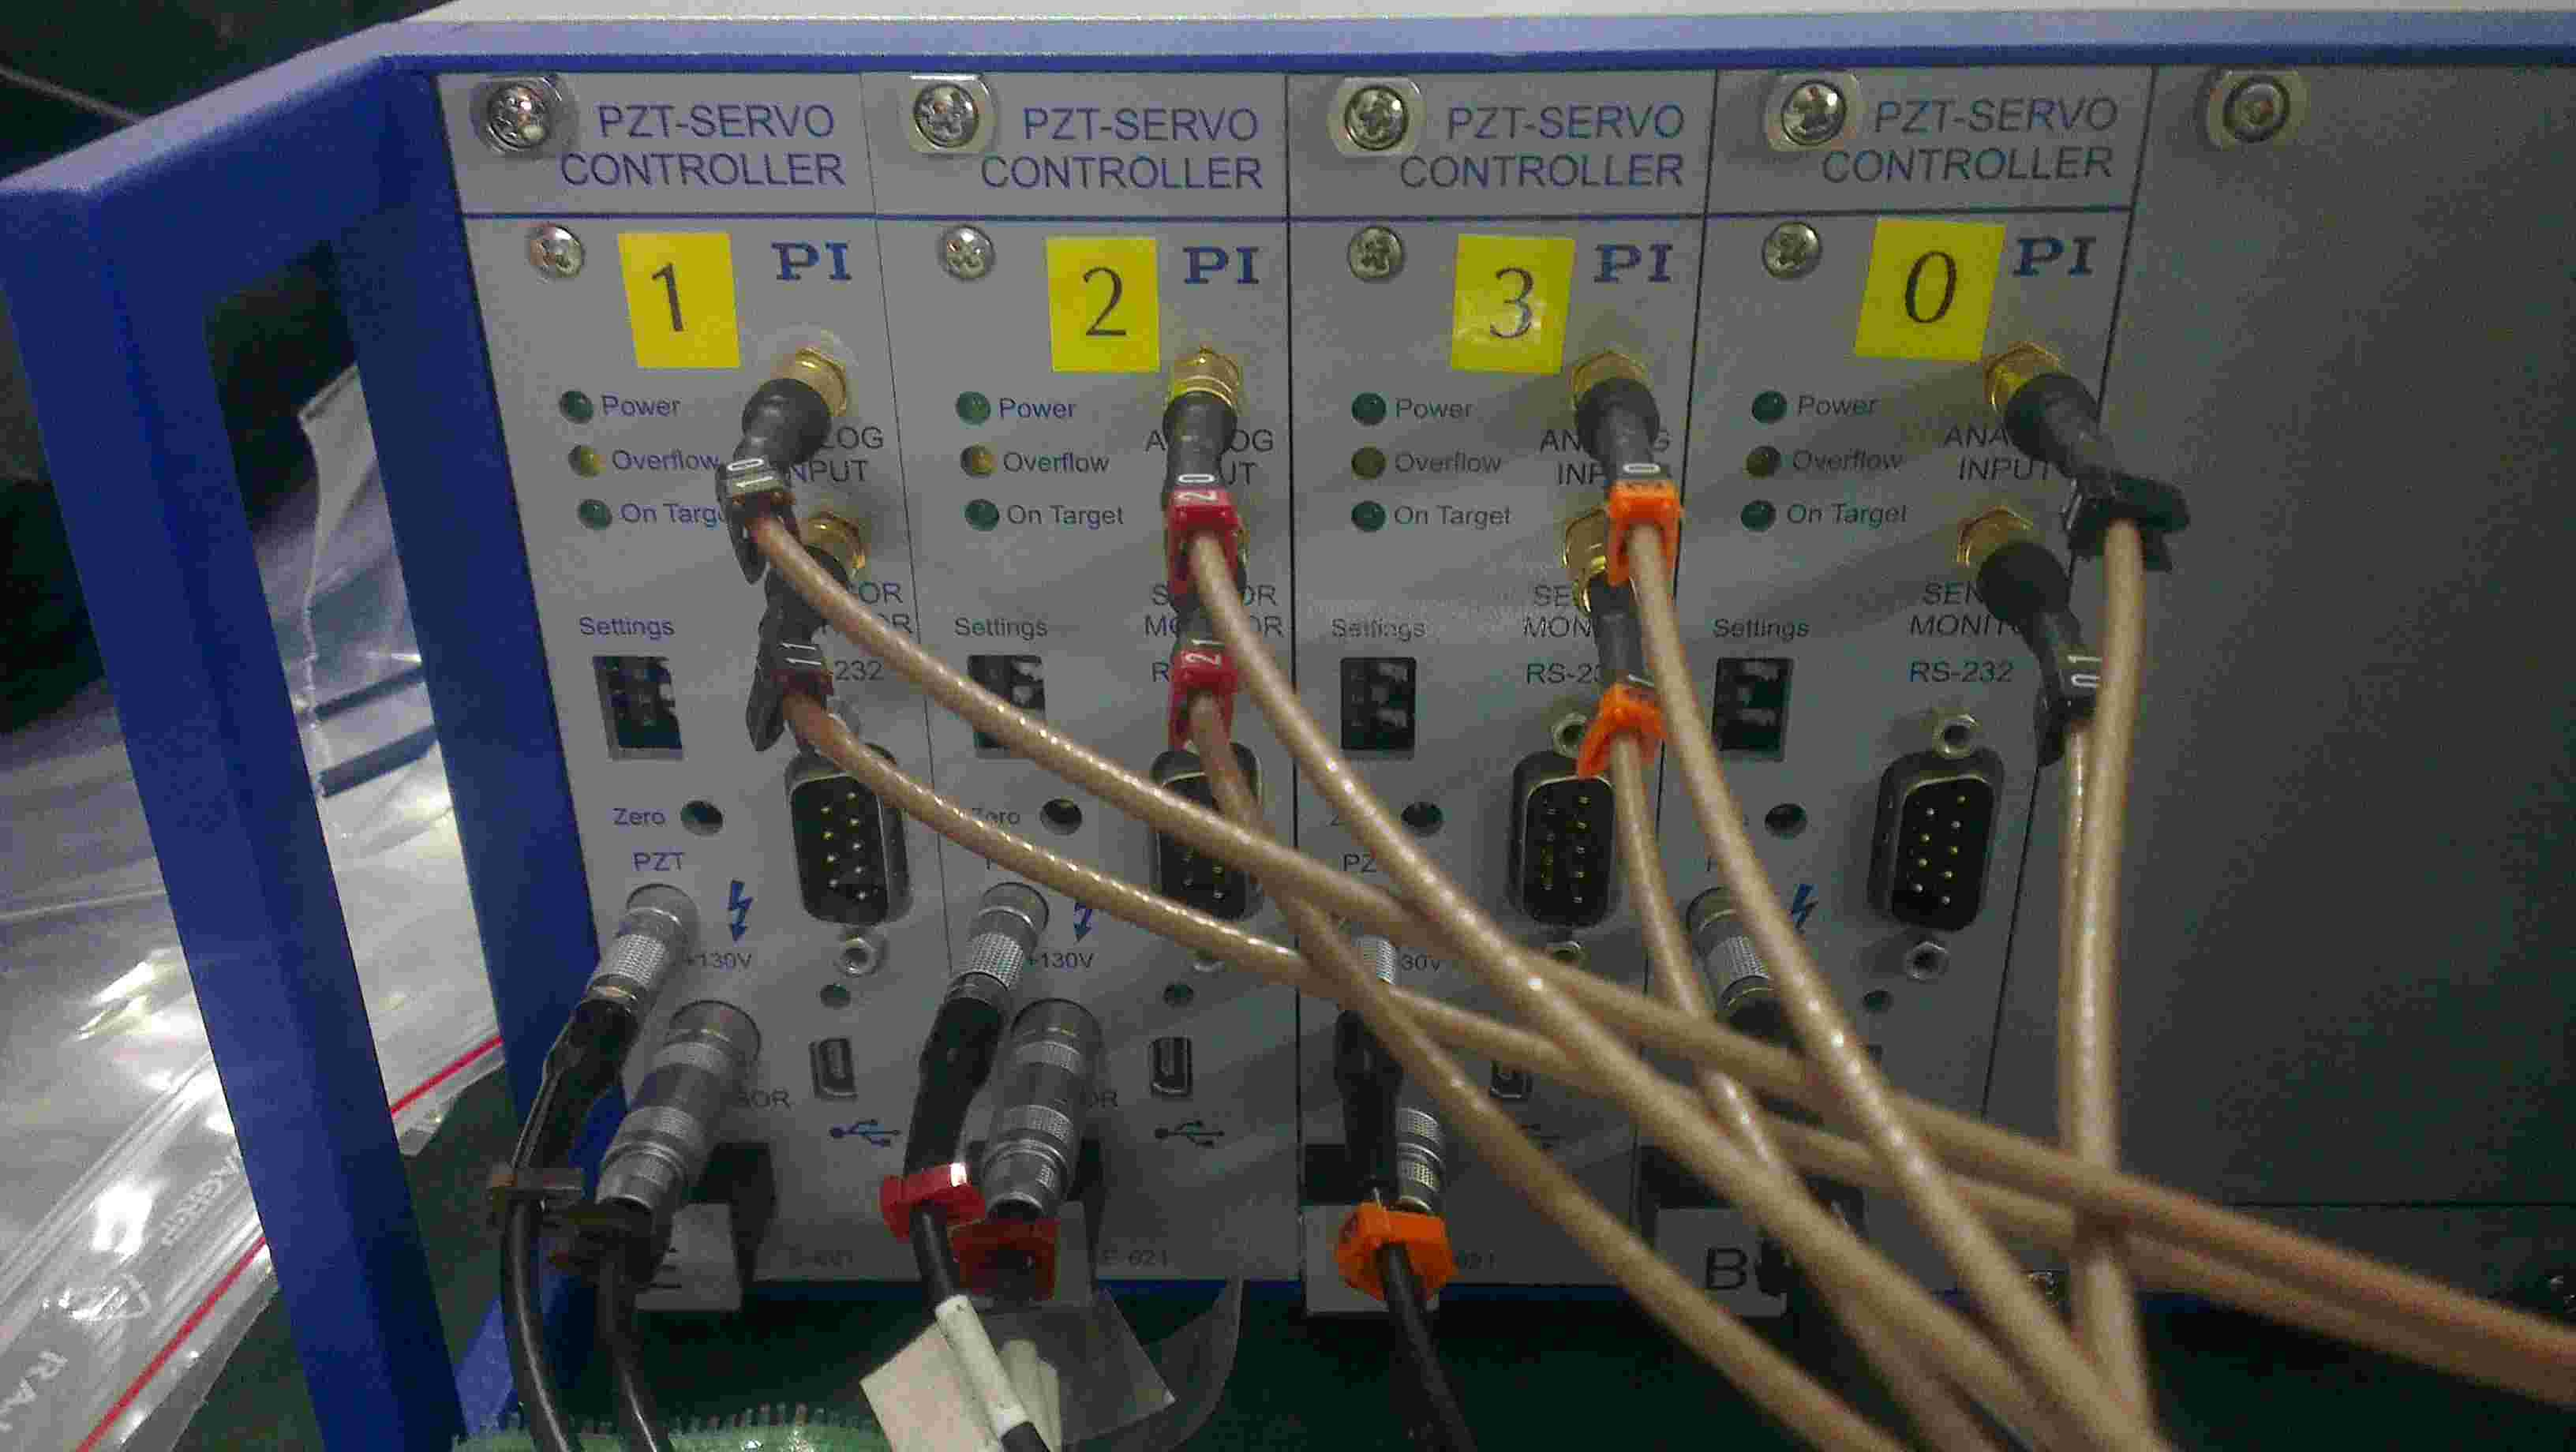
\includegraphics[height=1.6cm,width=3cm,angle=0]{ima04a.jpg}};
  \node (img5) at (2.0,0.0) {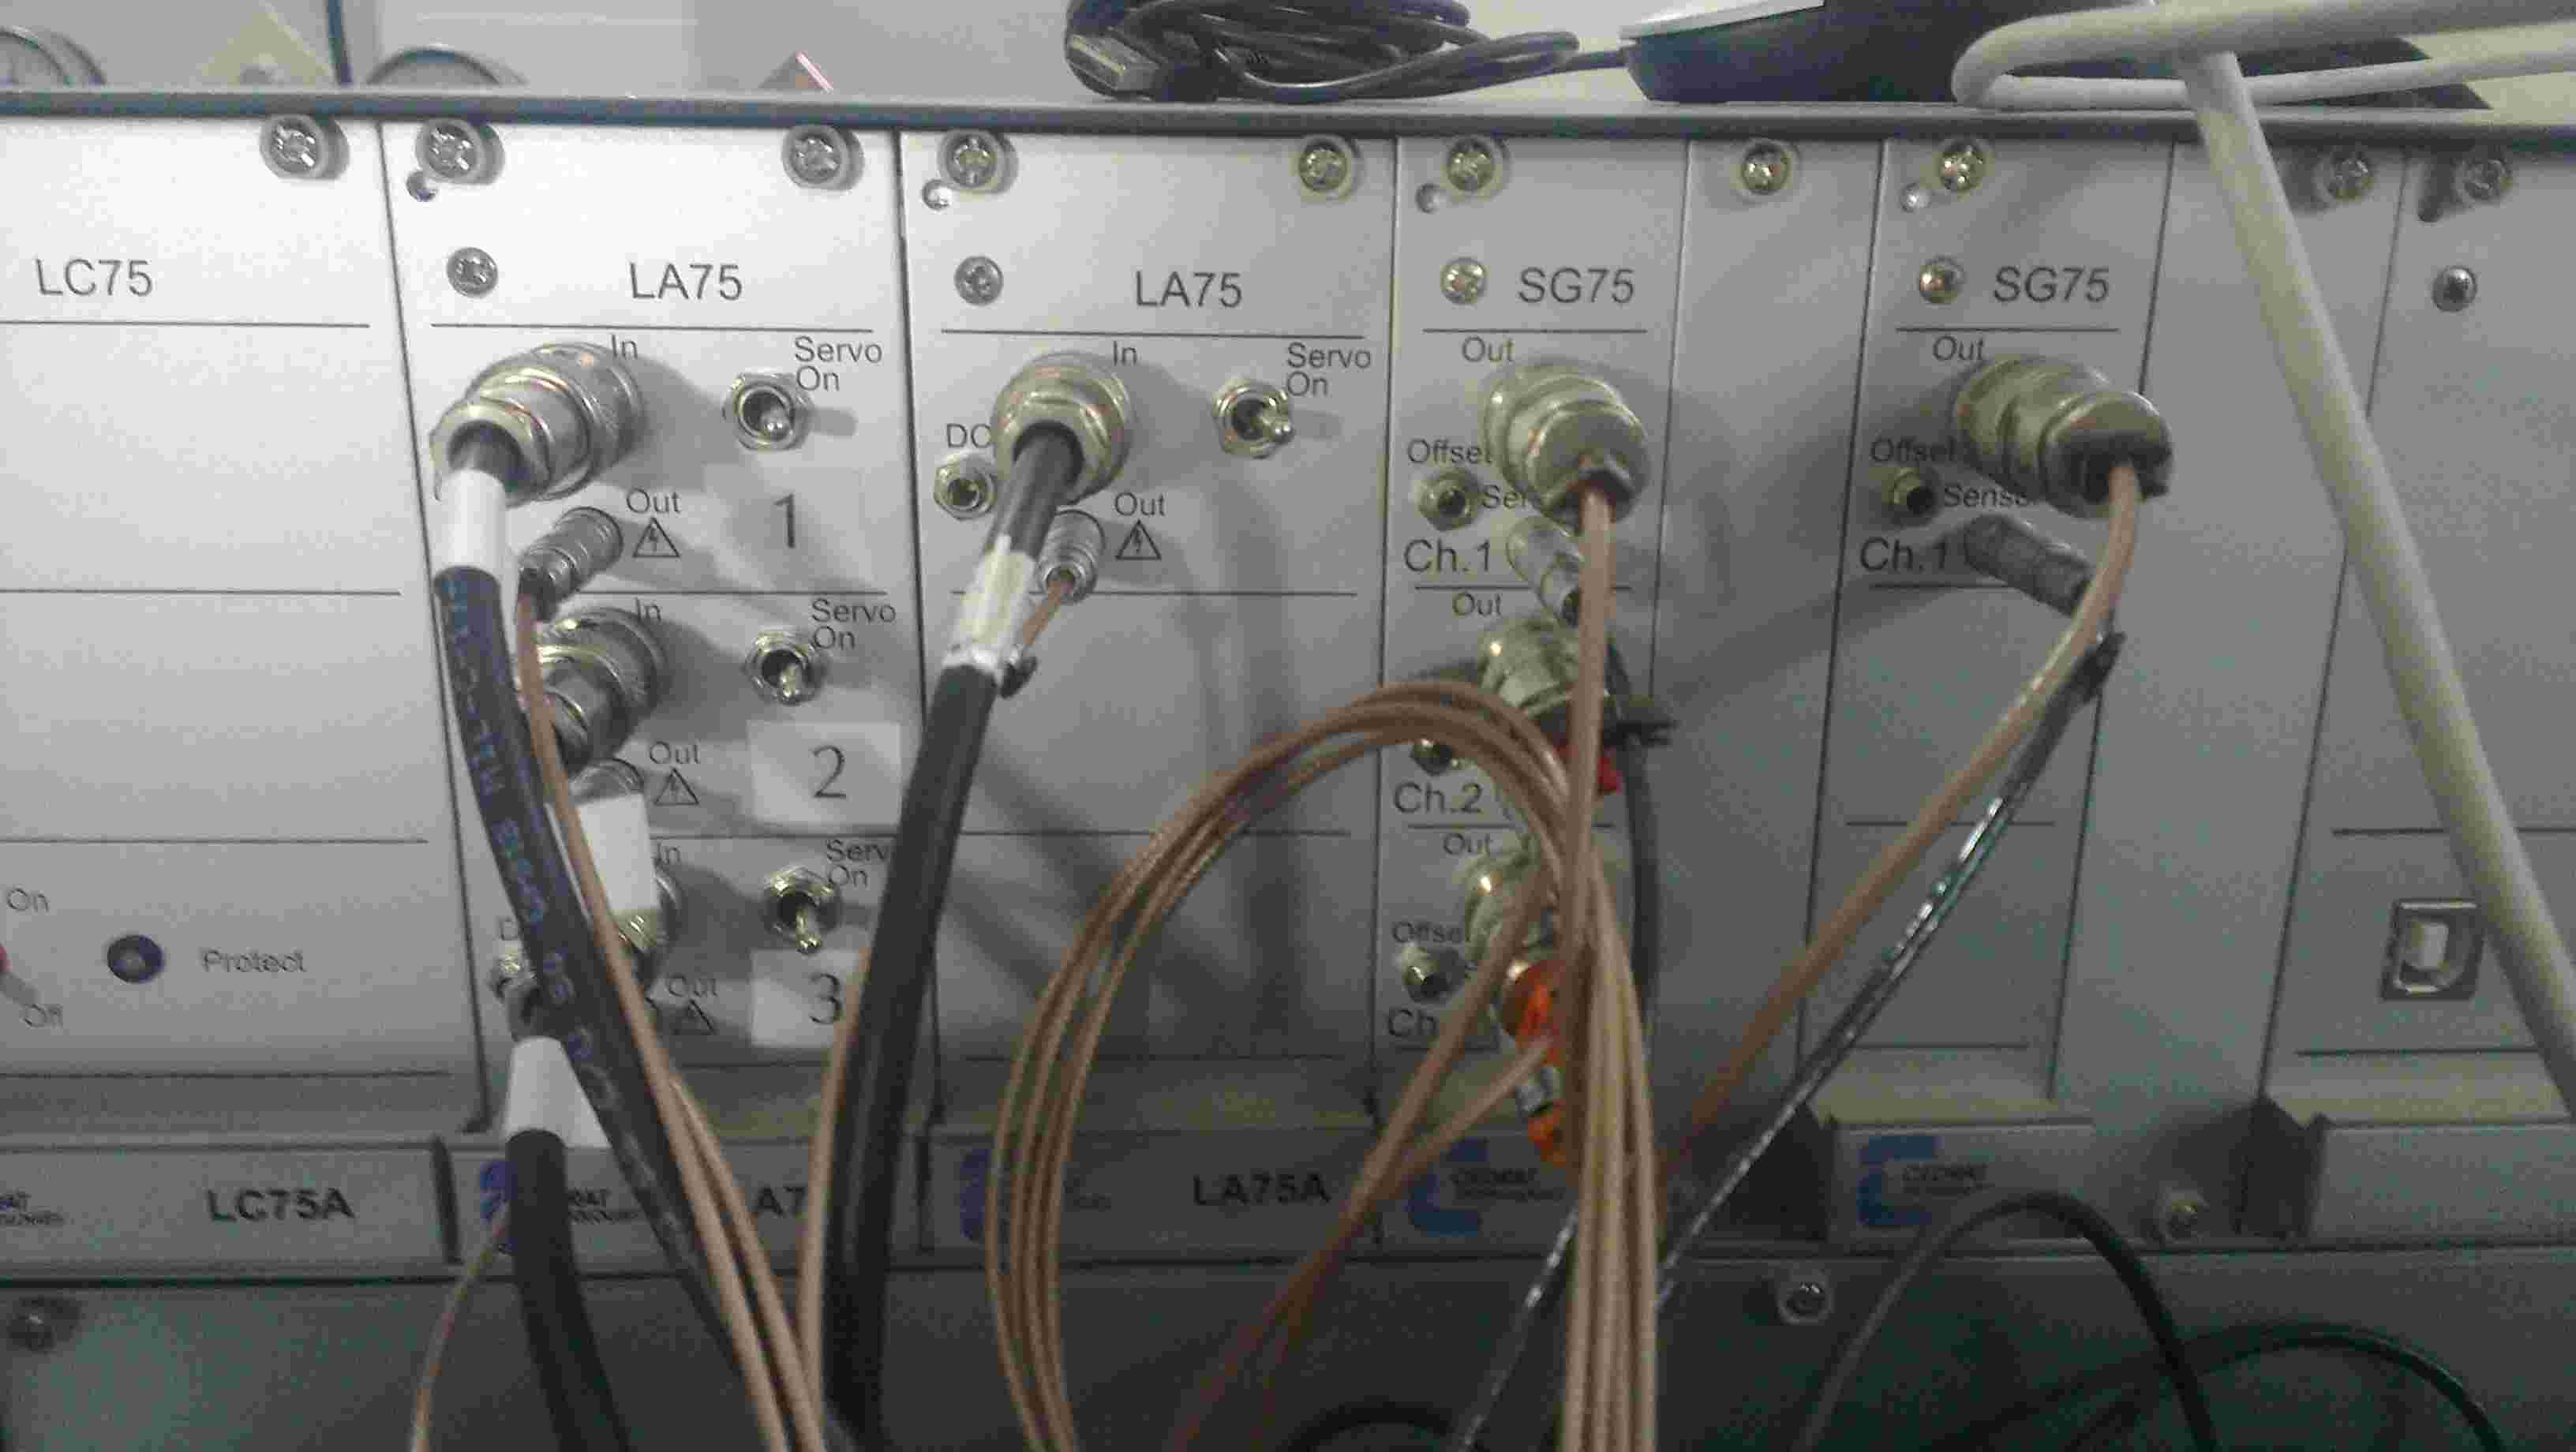
\includegraphics[height=1.6cm,width=3cm,angle=0]{ima05a.jpg}};
%   \pause
  \node (img6) at (4.4,3.0) {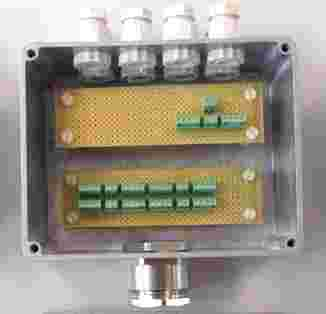
\includegraphics[height=1.6cm,width=3cm,angle=180]{ima08a.jpg}};
  \node (img7) at (1.8,1.4) {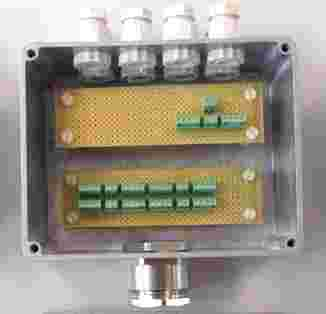
\includegraphics[height=1.6cm,width=3cm,angle=180]{ima08a.jpg}};
  \node (img8) at (1.8,3.0) {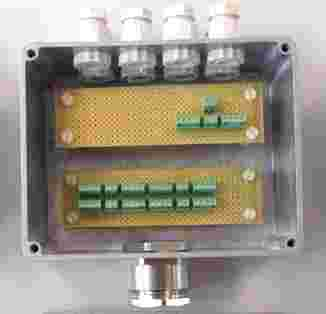
\includegraphics[height=1.6cm,width=3cm,angle=180]{ima08a.jpg}};
%   \pause
  \node (img9) at (-3.0,0.7)  {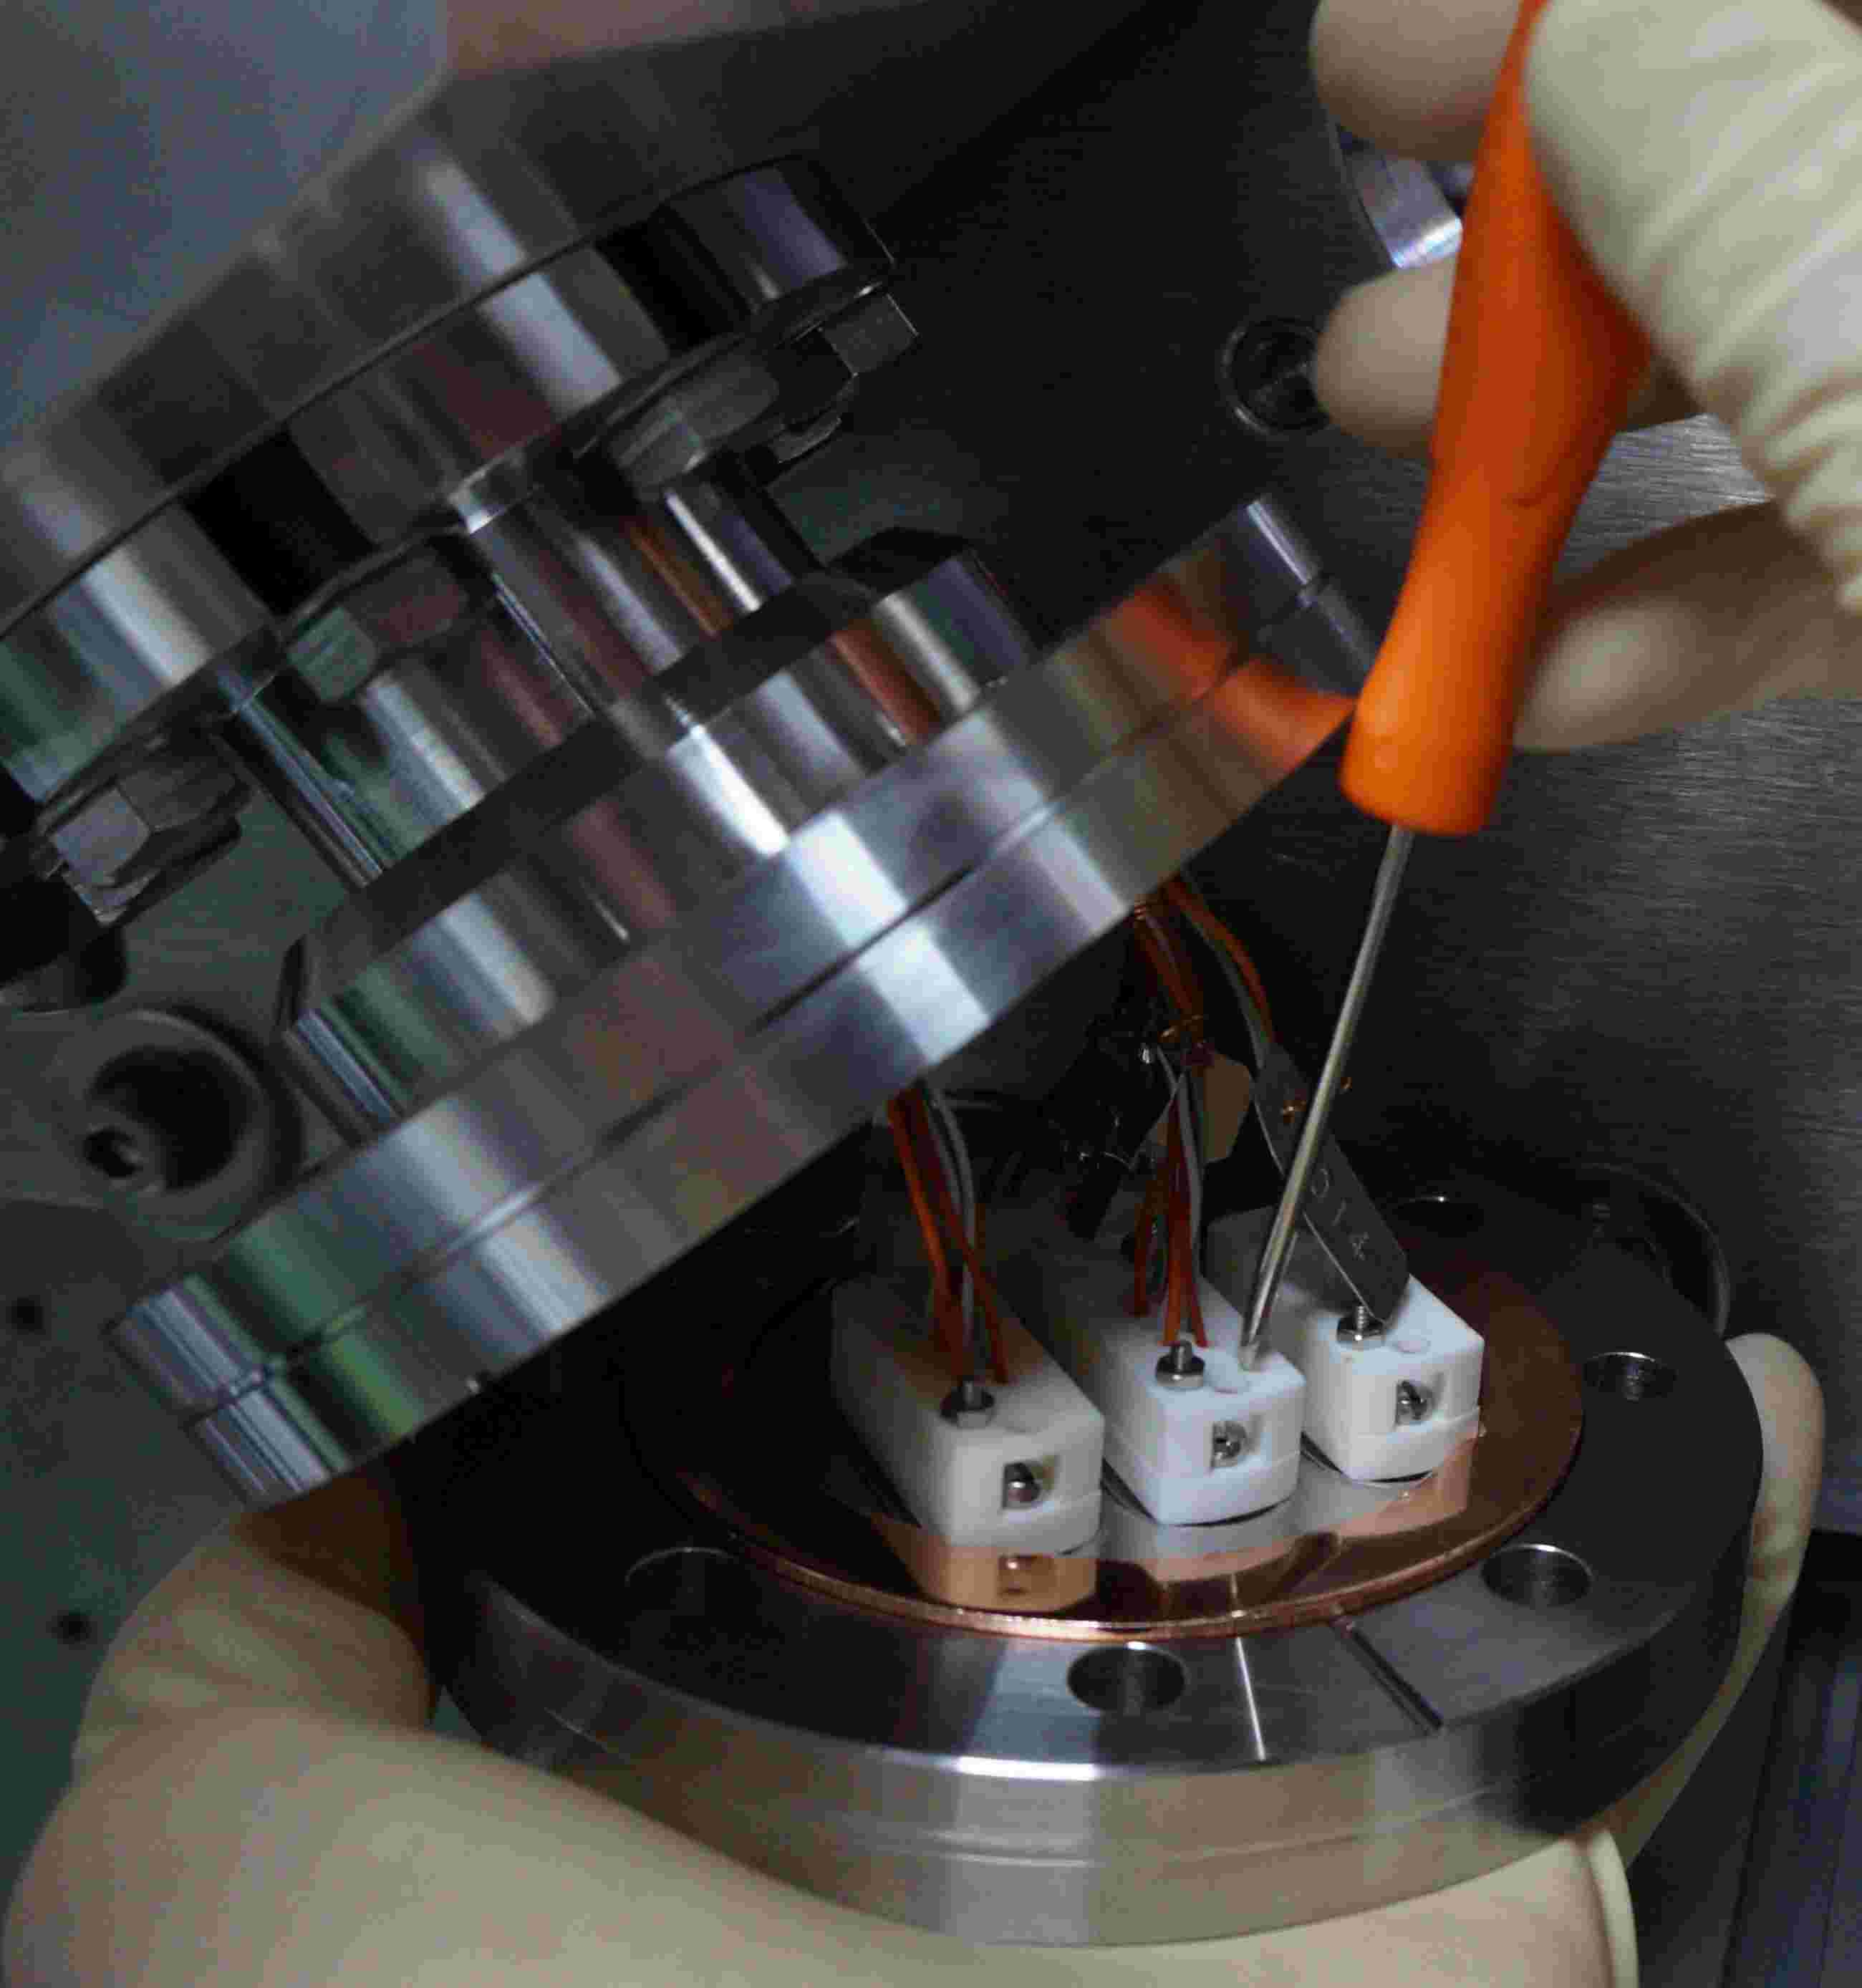
\includegraphics[height=1.6cm,width=1.4cm,angle=0]{ima10a.jpg}};
  \node (img10) at (-3.0,3.0) {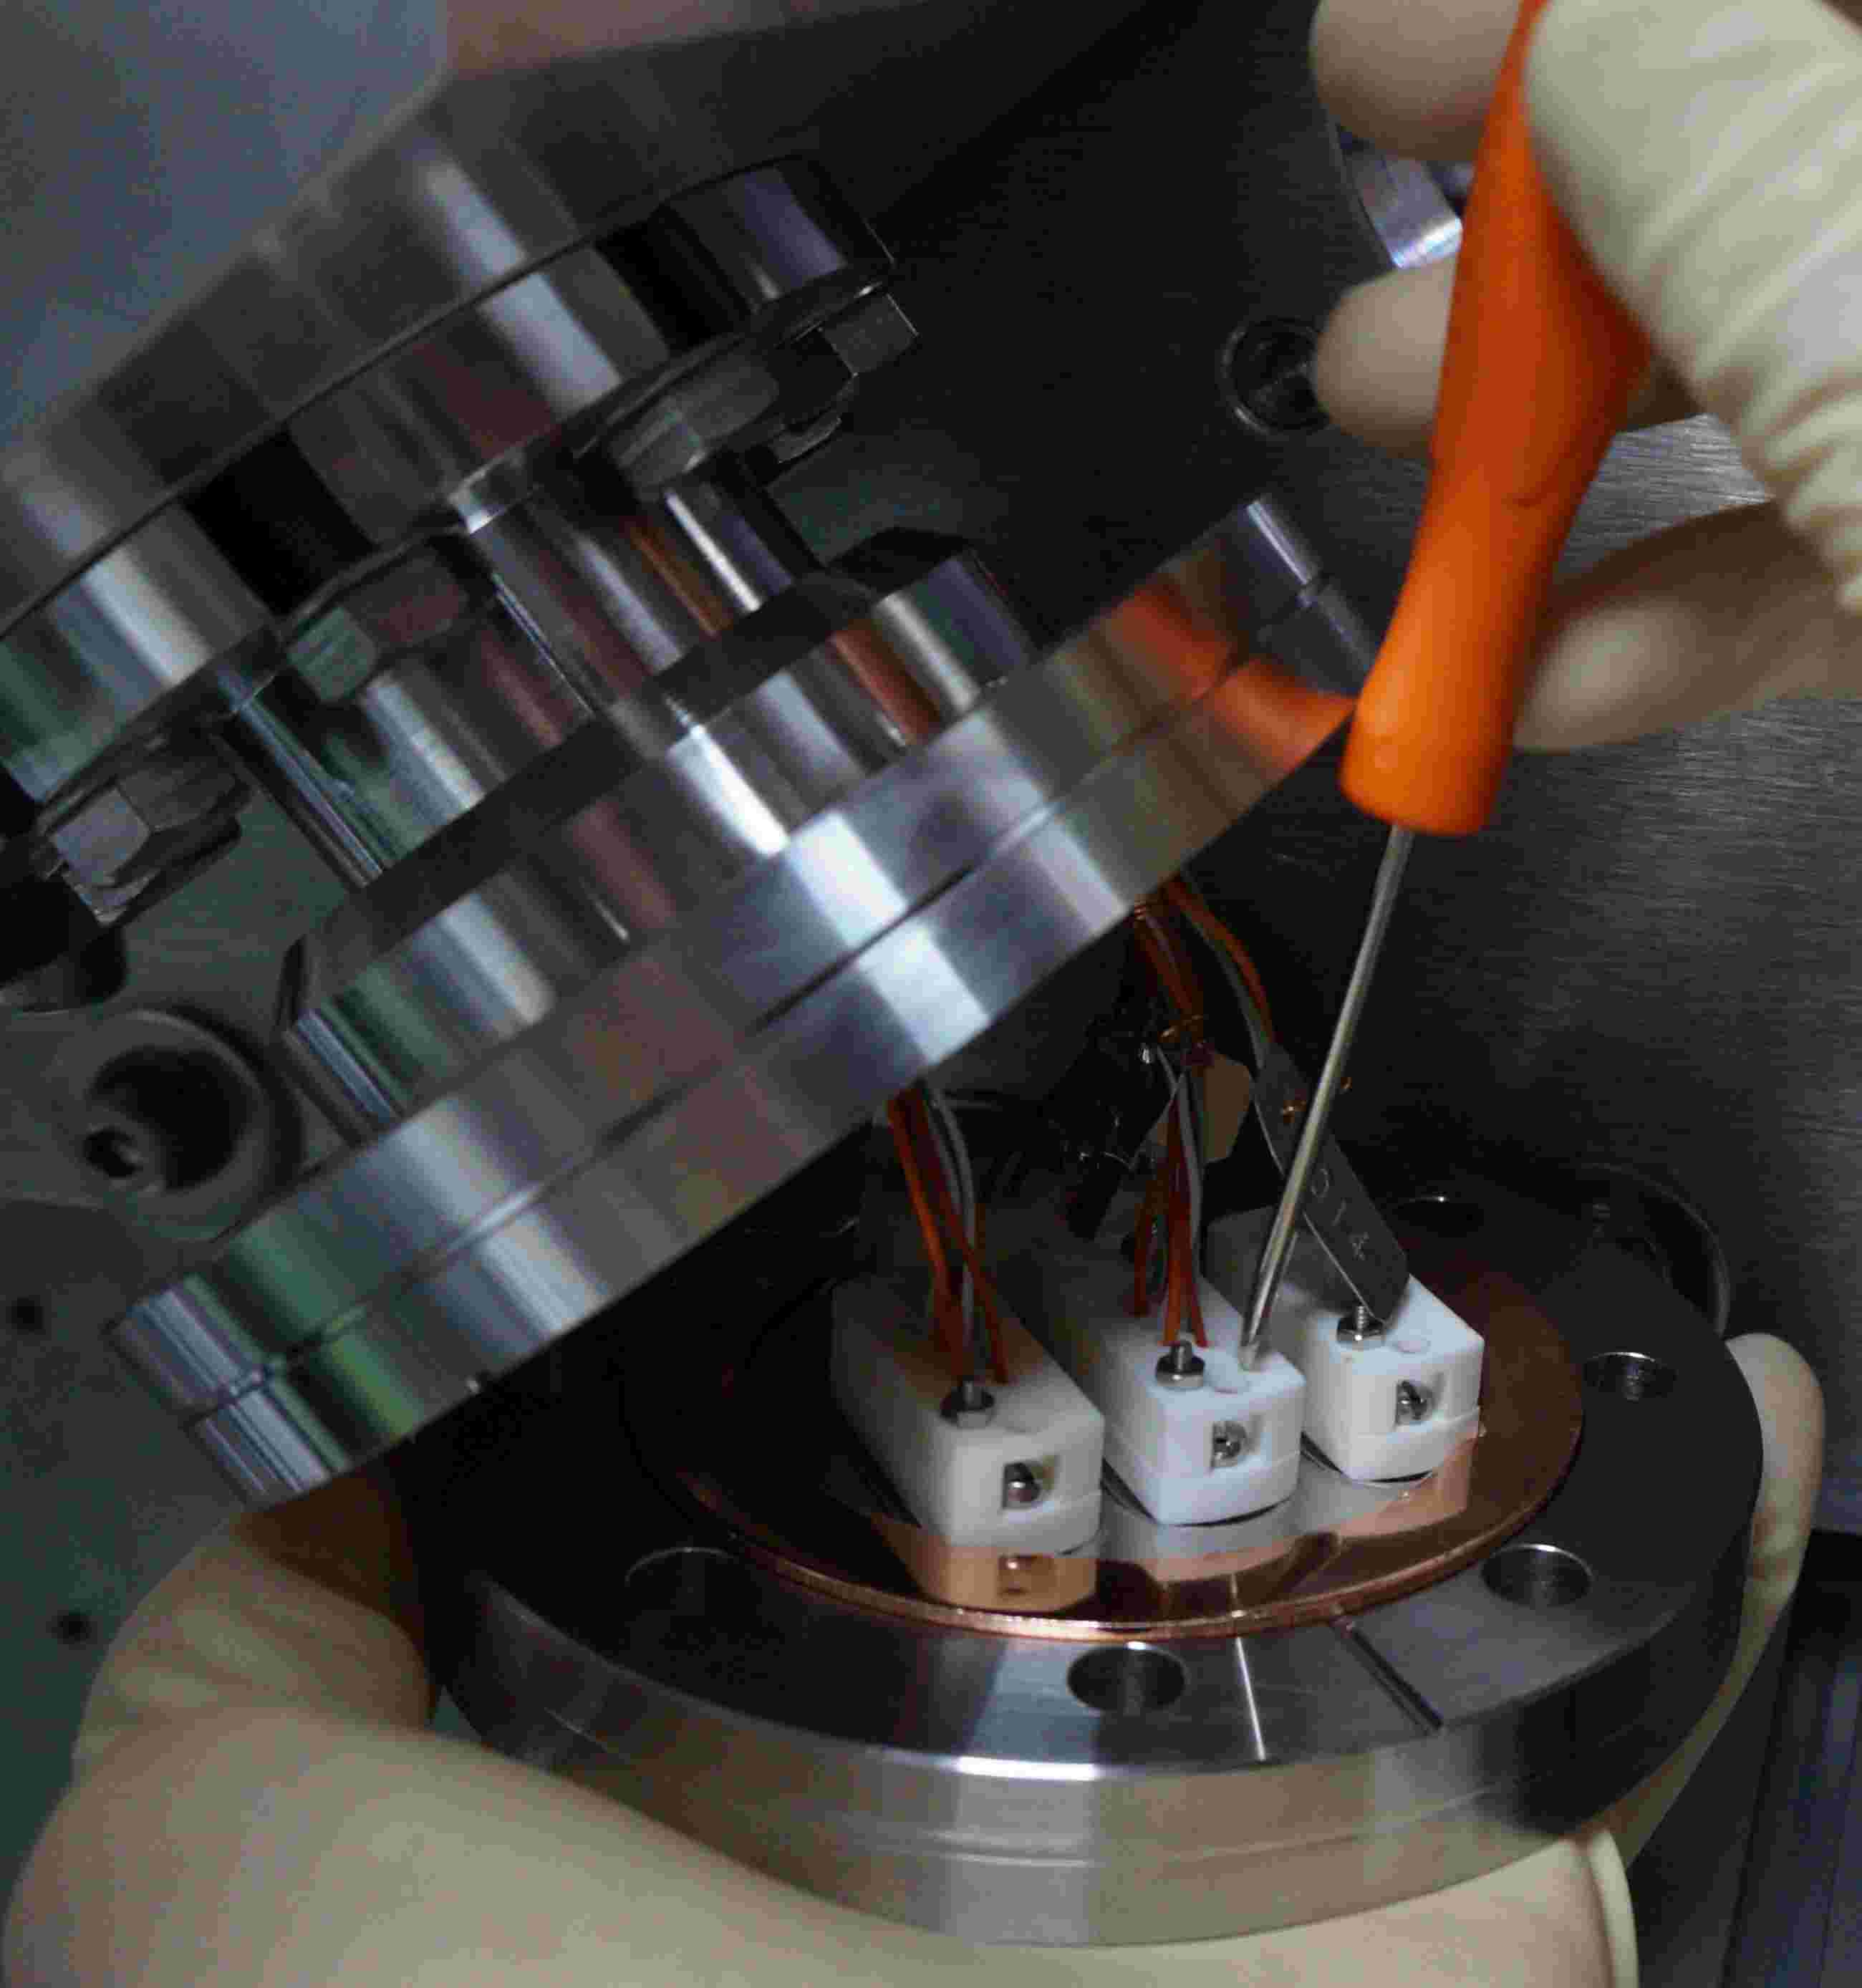
\includegraphics[height=1.6cm,width=1.4cm,angle=0]{ima10a.jpg}};
%   \pause
  \node (img11) at (-4.8,0.7)  {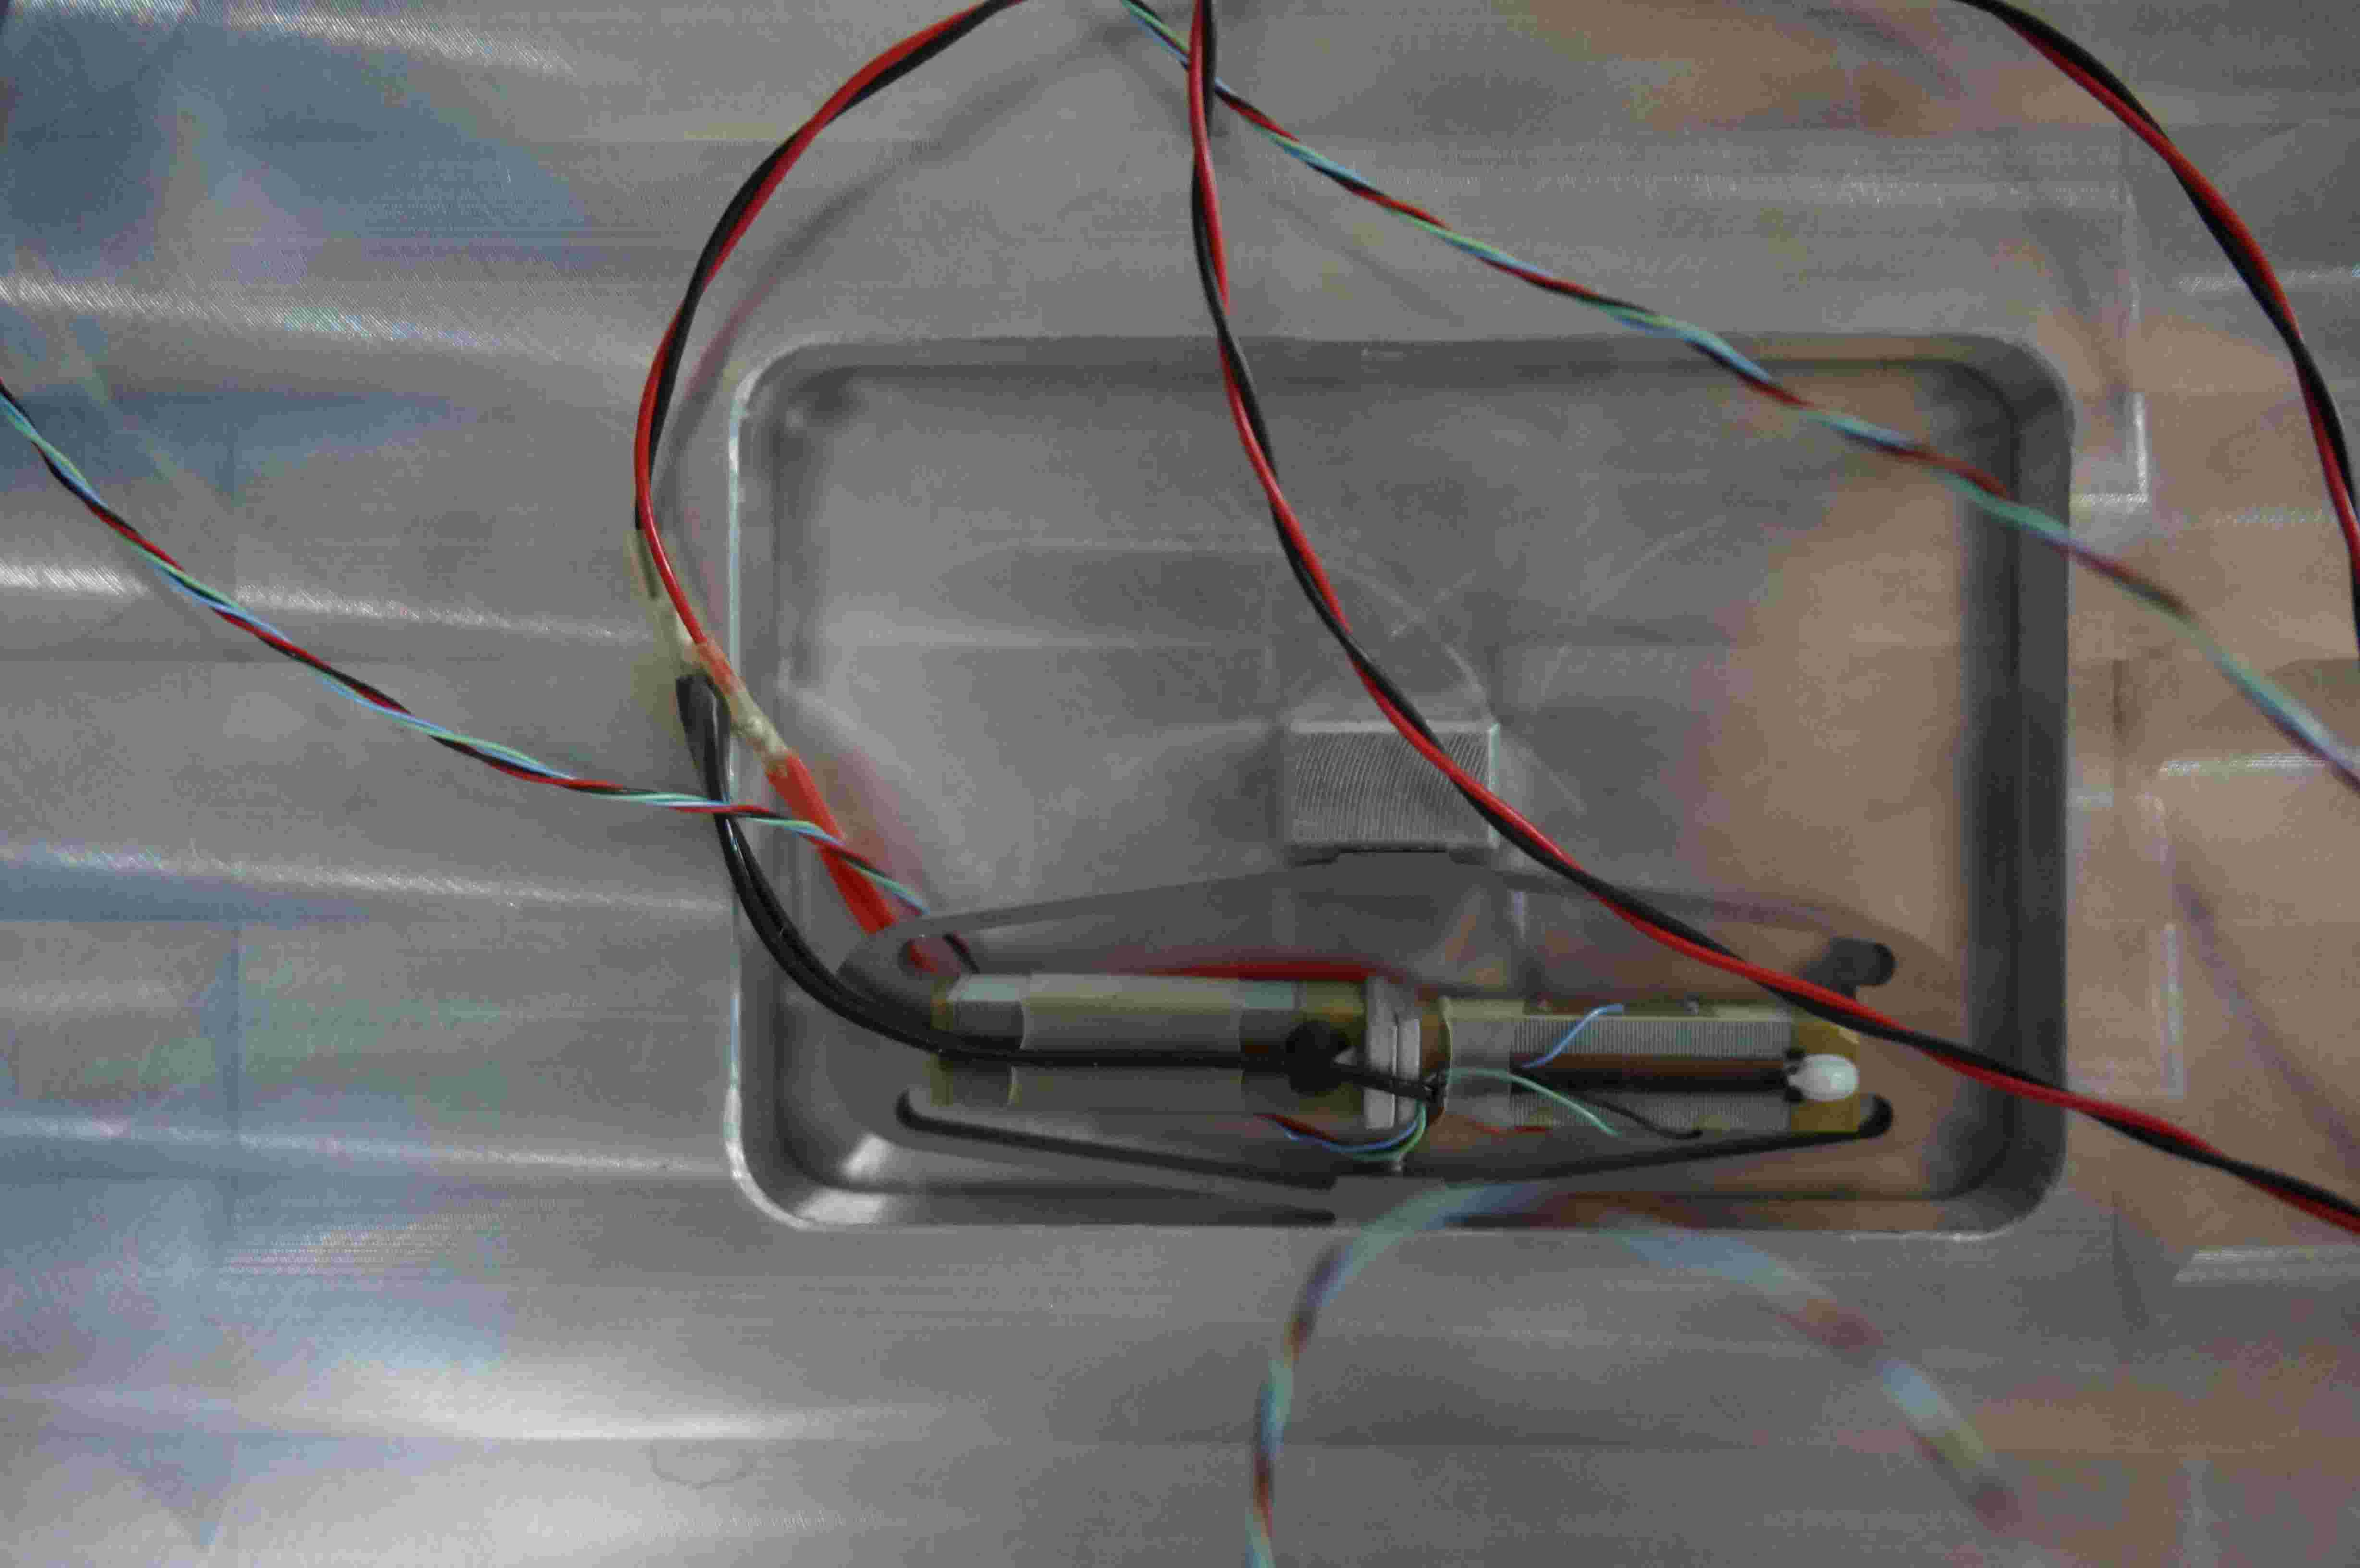
\includegraphics[height=1.6cm,width=1.4cm,angle=0]{ima11a.jpg}};
  \node (img12) at (-4.8,3.0) {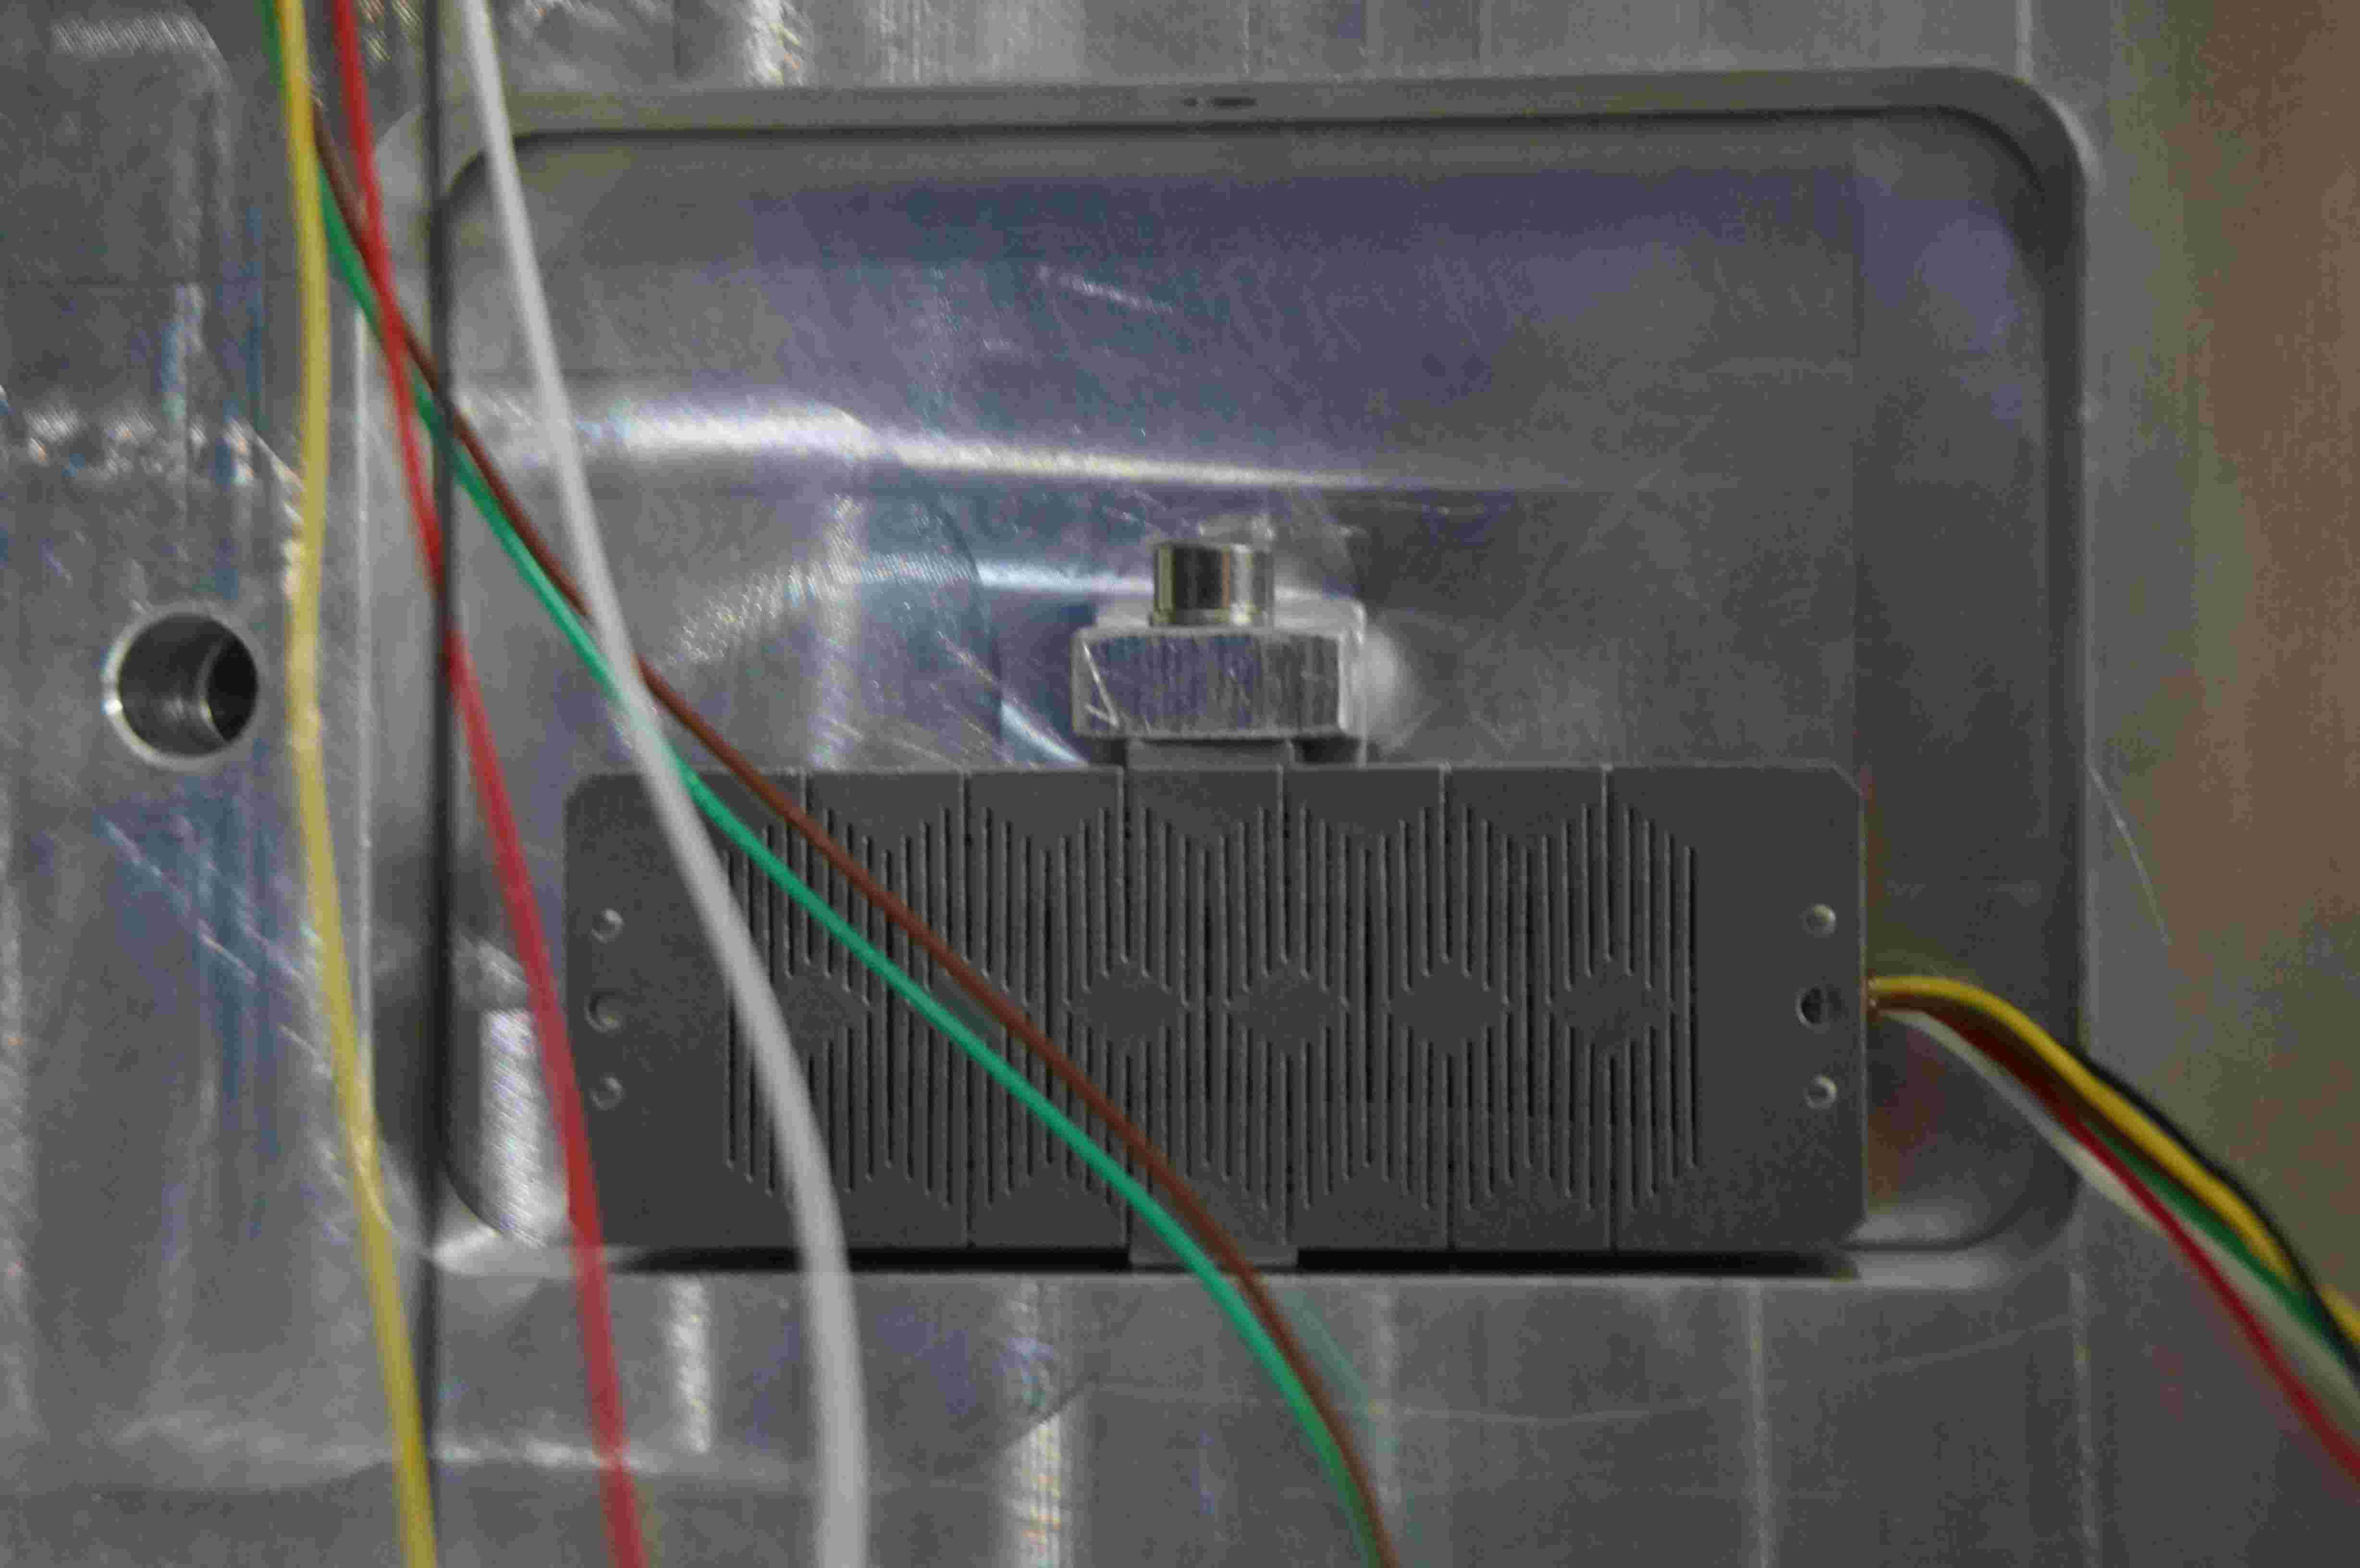
\includegraphics[height=1.6cm,width=1.4cm,angle=0]{ima12a.jpg}};
\end{tikzpicture}

\section{Mover Control}
Control per mover\par
\begin{center}
\begin{tikzpicture}
 \node (img1) {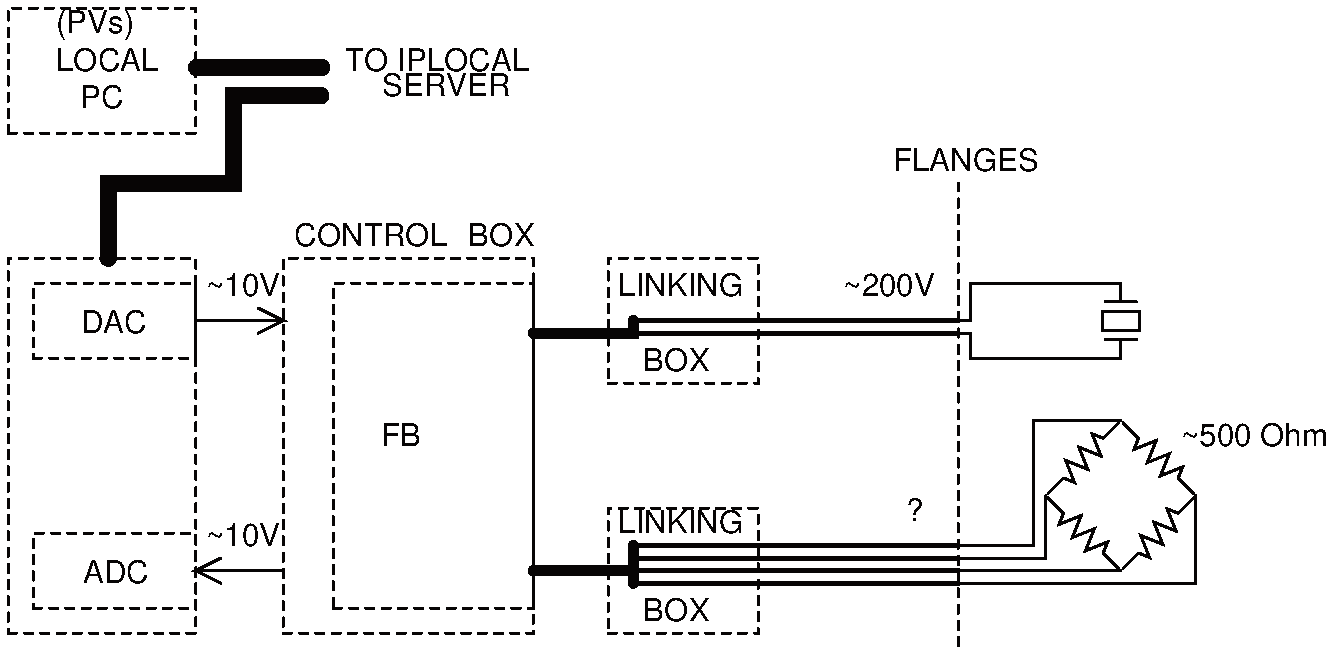
\includegraphics[scale=0.5]{Page1.pdf}};
 %\node (img2) at (4.4,1.5) {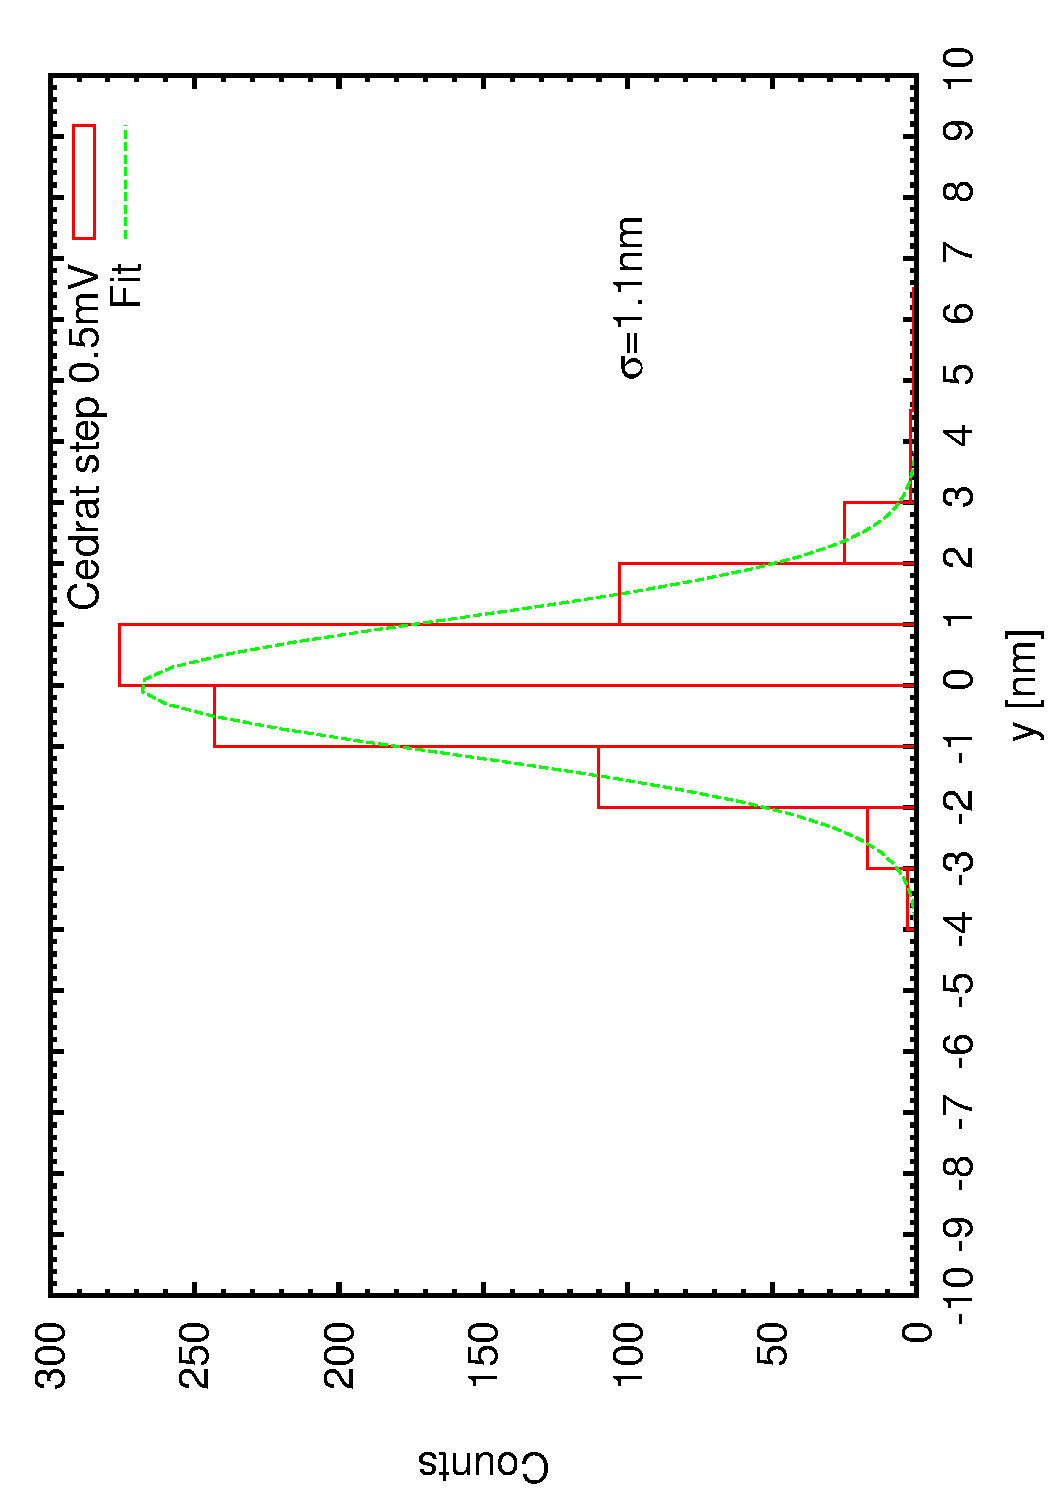
\includegraphics[scale=0.1,angle=-90]{imagestep12.pdf}};
%  \node (img3) at (4.4,2.6) {$\sigma_y=$?};
 %\node (img3) at (4.4,1.5) {{\LARGE\color{red} ?}};
\end{tikzpicture}
\end{center}
{\tiny BLOCK AB 1mV=31.25nm, BLOCK C 1mV=30nm}\par

\chapter{Operation}
\section{System Quick start}

Initialize the system\par
1. If any cable is hanging disconnected, first verify where it should be. All cables should be connected\par
2. Verify that PC and PLC are connected to network. During installation, both were connected to a hub and this was connected to ip-local.\par
3. PLC has no switch, it starts to work as soon it is connected and power is stable. If not connected, do this first. An orange LED will turn off when ready.\par
4. Cedrat has two ON switches. One in the back (main) and one in the front (connect and disconnects all input/outputs).\par
PI has one ON switch in the back.\par
PC (Laptop) has a switch on the front after opening the screen.\par
These three can be turn on in any order.\par
5. Let PI and Cedrat control electronics to heat up for 10 mins if first use during the day.\par
6. If the computer went to sleep or it is the first time in the day. It will be necessary to reinitialize the PLC. Follow these instructions.\par
1. Open the «National Instruments - Measurement \& Automation Explorer NI MAX«.\par
2. Select Périphériques et Interfaces\par
3. select Périphériques réseau.\par
4. If it is recognized, right-click over the peripheric and select «Réinitialiser le châssis«. A success prompt will appear some seconds after.\par
7. Open any of the previous programs designed in Labview to operate the system. Some of them can store the info in Excel format.\par
1. EPICS: if you are using EPICS, use the application:\par
"Bureau/Actionneurs Piezo/Applis Actionneurs positionnement BPMs - Ethernet - epics.vi" \par
2. Local system: use any of the avalaible applications\par

Shut down\par
1. Close all programs\par
2. Shut down PC, Cedrat and PI control electronics in any order.\par
PLC is left ON.\par
How to acquire data\par
When logged at atf-user.atf-local server, do:\par
To set voltage value:\par
Remember to use a PV which ends in Write.\par
Using one which ends in Read has no effect\par
\$ caput PVname Value\par
To get voltage from strain gauges:\par
Remember to use a PV which ends in Read.\par
Using one which ends in Write has no effect\par
\$ caget PVname\par
\$ camonitor Pvname (or PVnames)\par

\subsection{PVs}
NOTES\par
Epics PVs (Process Variables)\par
Write: sets a value on the DAC.\par
Read: reads from ADC.\par
Channels IP:BPM-AB:Mover0 and IP:BPM-C:MoverB are for lateral movement.\par

IP:BPM-AB:Mover0:Read\par
IP:BPM-AB:Mover0:Write\par
IP:BPM-AB:Mover1:Read\par
IP:BPM-AB:Mover1:Write\par
IP:BPM-AB:Mover2:Read\par
IP:BPM-AB:Mover2:Write\par
IP:BPM-AB:Mover3:Read\par
IP:BPM-AB:Mover3:Write\par 

IP:BPM-C:MoverB:Read\par 
IP:BPM-C:MoverB:Write\par 
IP:BPM-C:MoverC:Read\par 
IP:BPM-C:MoverC:Write\par 
IP:BPM-C:MoverD:Read\par 
IP:BPM-C:MoverD:Write\par 
IP:BPM-C:MoverE:Read\par 
IP:BPM-C:MoverE:Write\par 

IP:BPM-AB:Temp\par 
IP:BPM-C:Temp\par 

Older Epics PVs, DO NOT USE (Process Variables)\par 
These PVs are here for documentation purposes. They are still functional but any new work should be done with previously defined PV in this document.\par 
Write: sets a value on the DAC.\par 
Read: reads from ADC.\par 
Channels Cedrat0 and PIB are for lateral movement.\par 

IPBSM:BPMs:PIB:Write\par 
IPBSM:BPMs:PIB:Read\par 
IPBSM:BPMs:PIC:Write\par 
IPBSM:BPMs:PIC:Read\par 
IPBSM:BPMs:PID:Write\par 
IPBSM:BPMs:PID:Read\par 
IPBSM:BPMs:PIE:Write\par 
IPBSM:BPMs:PIE:Read\par 


IPBSM:BPMs:Cedrat0:Write\par 
IPBSM:BPMs:Cedrat0:Read\par 
IPBSM:BPMs:Cedrat1:Write\par 
IPBSM:BPMs:Cedrat1:Read\par 
IPBSM:BPMs:Cedrat2:Write\par 
IPBSM:BPMs:Cedrat2:Read\par 
IPBSM:BPMs:Cedrat3:Write\par 
IPBSM:BPMs:Cedrat3:Read\par 

Read temperature:\par 
IPBSM:BPMs:Temp1\par 
IPBSM:BPMs:Temp2\par 

\subsection{Troubleshooting}
Q/A and Troubleshooting\par 
Is there any connection problem with the chassis?\par 
A1: Check voltage and network cable connection. If status led is in orange it stills need sometime to operate.\par 
A2: Open the «National Instruments - Measurement \& Automation Explorer NI MAX«. Select Périphériques et Interfaces, select Périphériques réseau. If it is recognized, right-click over the peripheric and select «Réinitialiser le châssis«. A success prompt will appear some seconds after.\par 
A3: If the ni9188 appears, but you are not able to set (unset) parameters. Push the reset button in the chassis for at least 5 seconds. It will set all parameters to default.\par 
A4: If you still have problems, disconnect all cables for at least 10 seconds and reconnect.\par 
A5: If required the PLC can connect directly with the PC via network cable (no crossing). Reset all parameters and reconnect.\par 

Are values at the readback different from the voltage set?\par 
A1: it is normal to have a difference up to milivolts. Difference might be larger at the extreme points in PI and in the middle range for CEDRAT.\par 
A2: If difference is larger, it is possible that feedback system is not connected. In doubt  consult the corresponding manual.\par 
A3: Normally all front lights in PI and CEDRAT system should be green. If not, there is a electrical problem. Most common situation is that something is disconnected. Labels have been placed per cable in order to easily identify where does it belongs.\par 
A4: Check power voltage and compare with the operation ranges at the back of PI and CEDRAT equipment. During the installation, 220V connectors were used.\par 
A5: Try to check that the value set by the Labview system corresponds to the value converted by the DAC. You can use a multimeter or use the ADC to test the PC-DAC-ADC chain.\par 

Feedback\par 
A1. It is possible to make adjustments on fb. Both, PI and CEDRAT. \par 
Procedure is simpler in CEDRAT, you have to connect the PC to the Cedrat electronics USB connection. Open the program «HDPM45v16.vi», and update P, I and D control values. It requires some seconds to update the info. More specifications, consult manual.\par 
PI: it is possible to change the feedback parameter. In order to do it, an additional board is required. Contact Laboratoire de L'accélérateur Lineaire (LAL).
A2. If the led OVERFLOW is on. There is a cable problem. Either it is disconnected or connected to the wrong channel and the feedback goes to an overflow.\par 
A3. CEDRAT Led is red. Cables are not correctly connected, verify the high tension cables specially. Each cable is identified with a number that has been engraved in the chamber lower flanges.\par 

Temperature.\par 
A1. Channels 0 (Cedrat) and 2 (PI) are connected to the NI 9219. If no lecture verify network connection.\par 
A2: 0.8 to 0.4 degC difference was observed during the installation between both channels. Reasons are still under study.\par 

Ground connection\par 
A1: Ground connection is common to all dispositives. \par 
\mainmatter
\chapter{Status}
\section{Linearity}
\subsection{Vertical displacement}
Measuring system\par
An interferometer was used to measure BPM position. As the head is located over the BPM, positive displacement implies negative change in the intereferometer lecture.\par
\hspace*{1.4cm}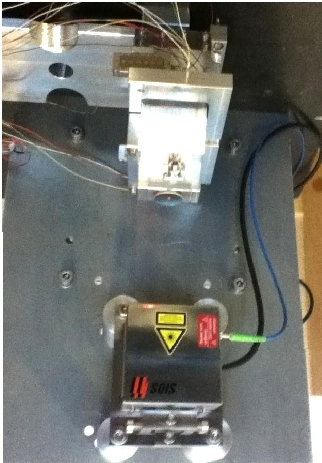
\includegraphics[angle=180,scale=0.2]{interfero.jpg}\par
\begin{figure}[htb]
\centering
 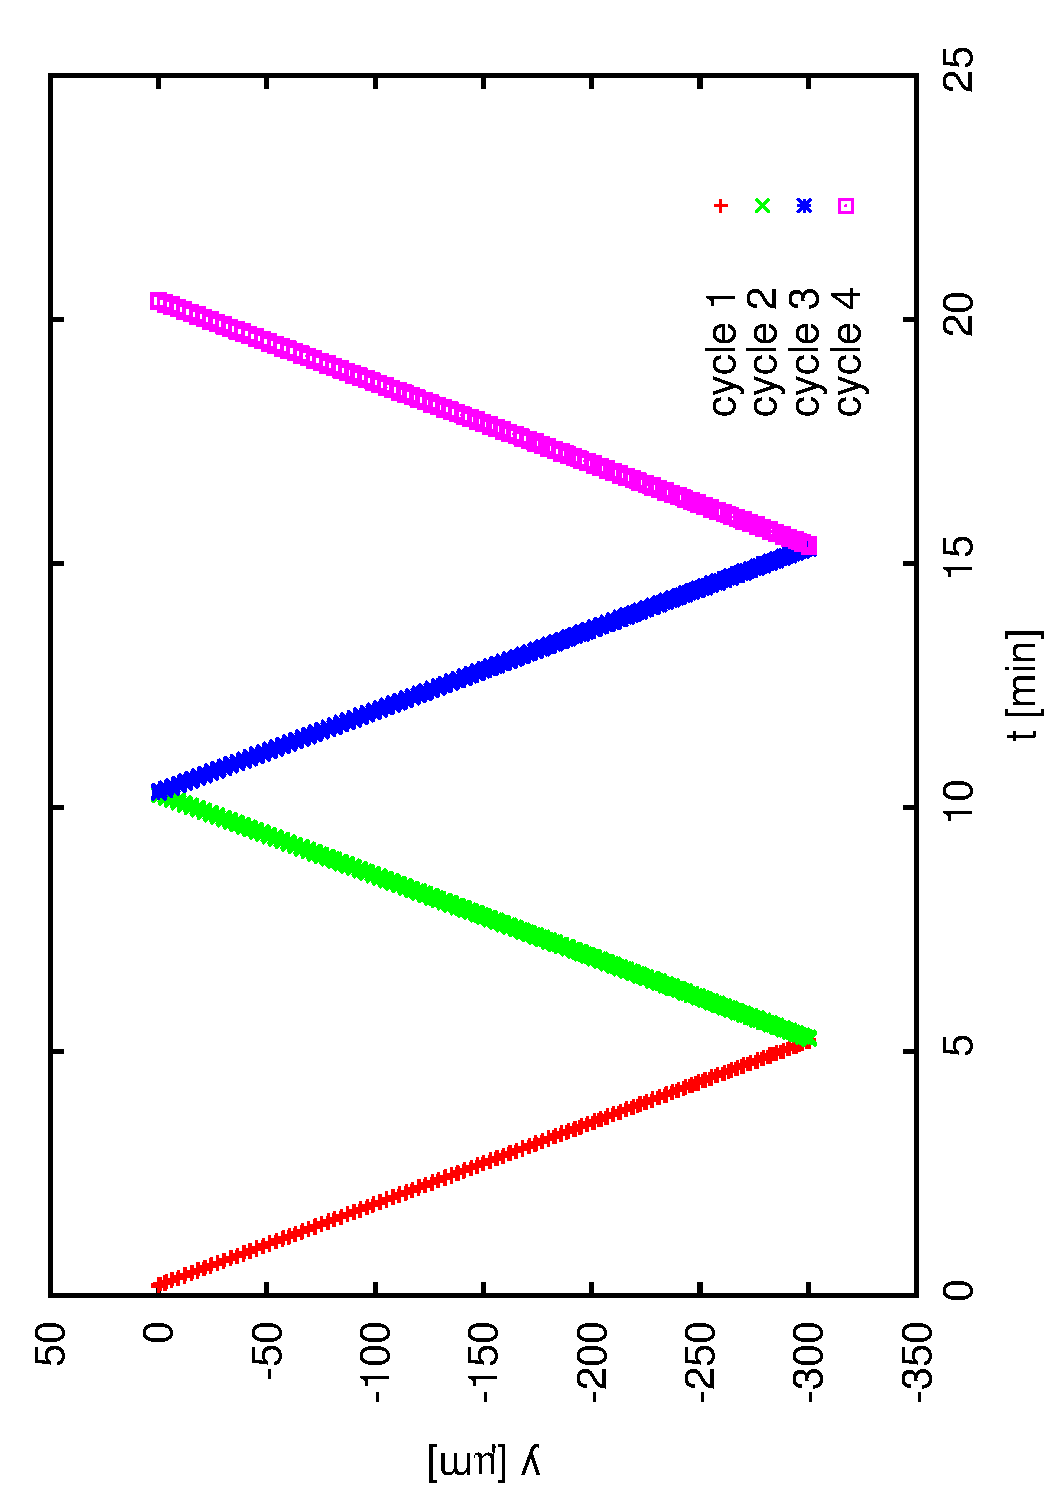
\includegraphics[scale=0.3,angle=-90]{image01.pdf}\caption{PI movers linearity}\label{f-LinPI01}
\end{figure}
\subsubsection{PI without and with feedback}
Four cycles (two going up, two going down),
range (0$\sim$10V, 0$\sim$300$\mu$m)\par
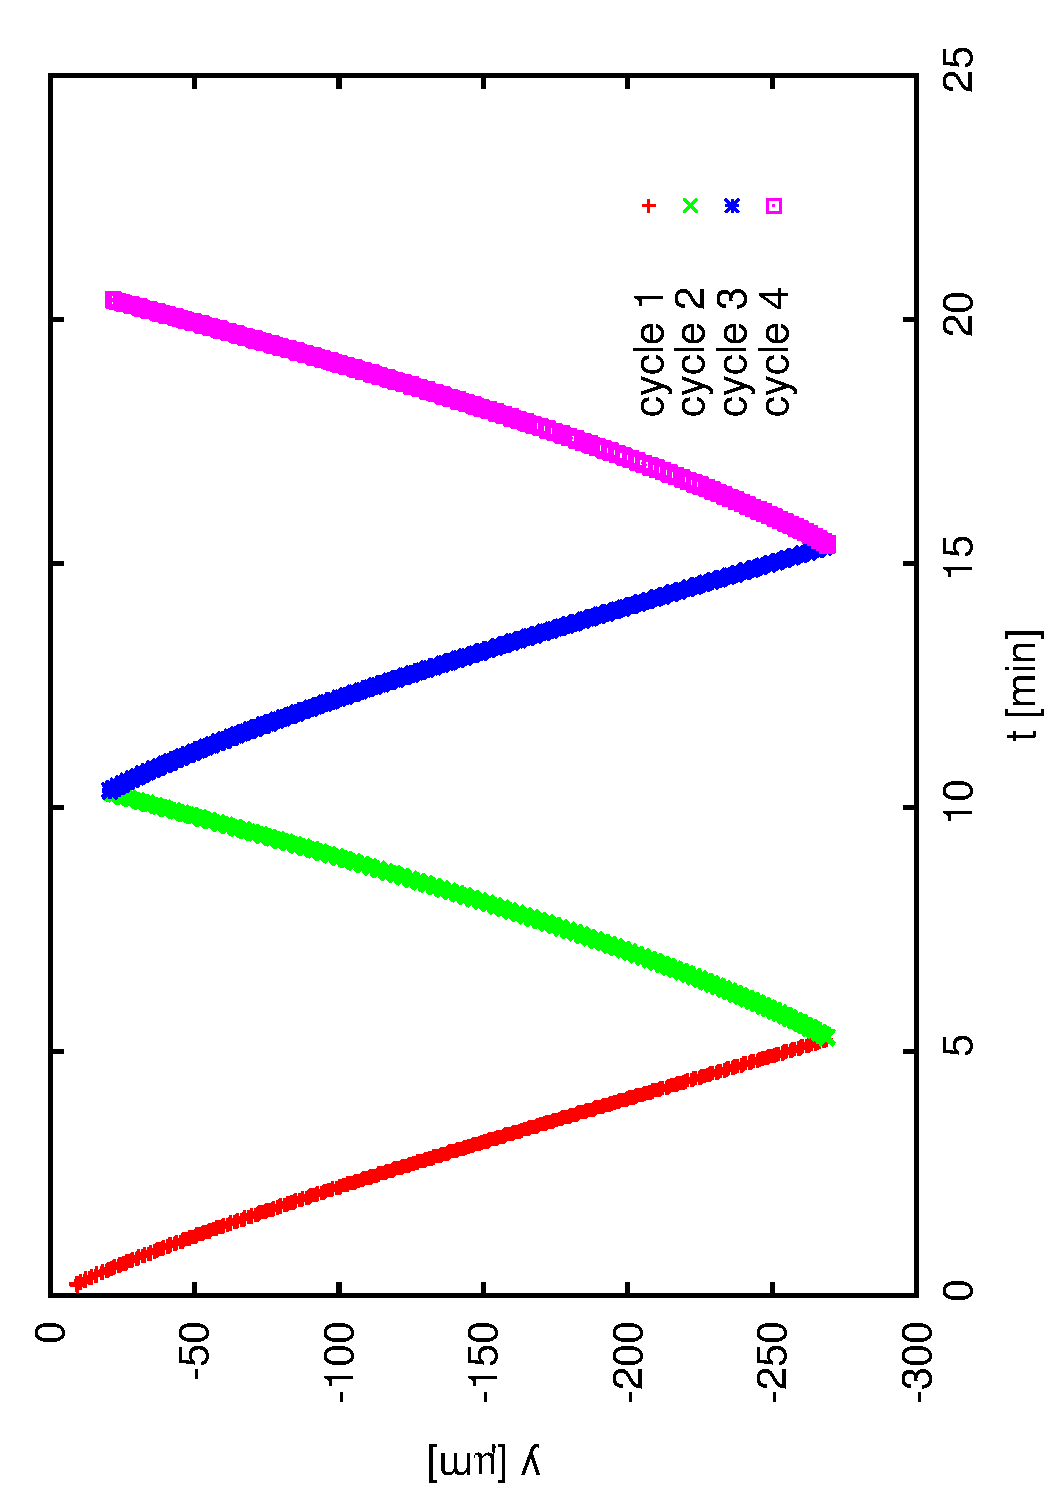
\includegraphics[angle=-90,scale=0.15]{image11.pdf}
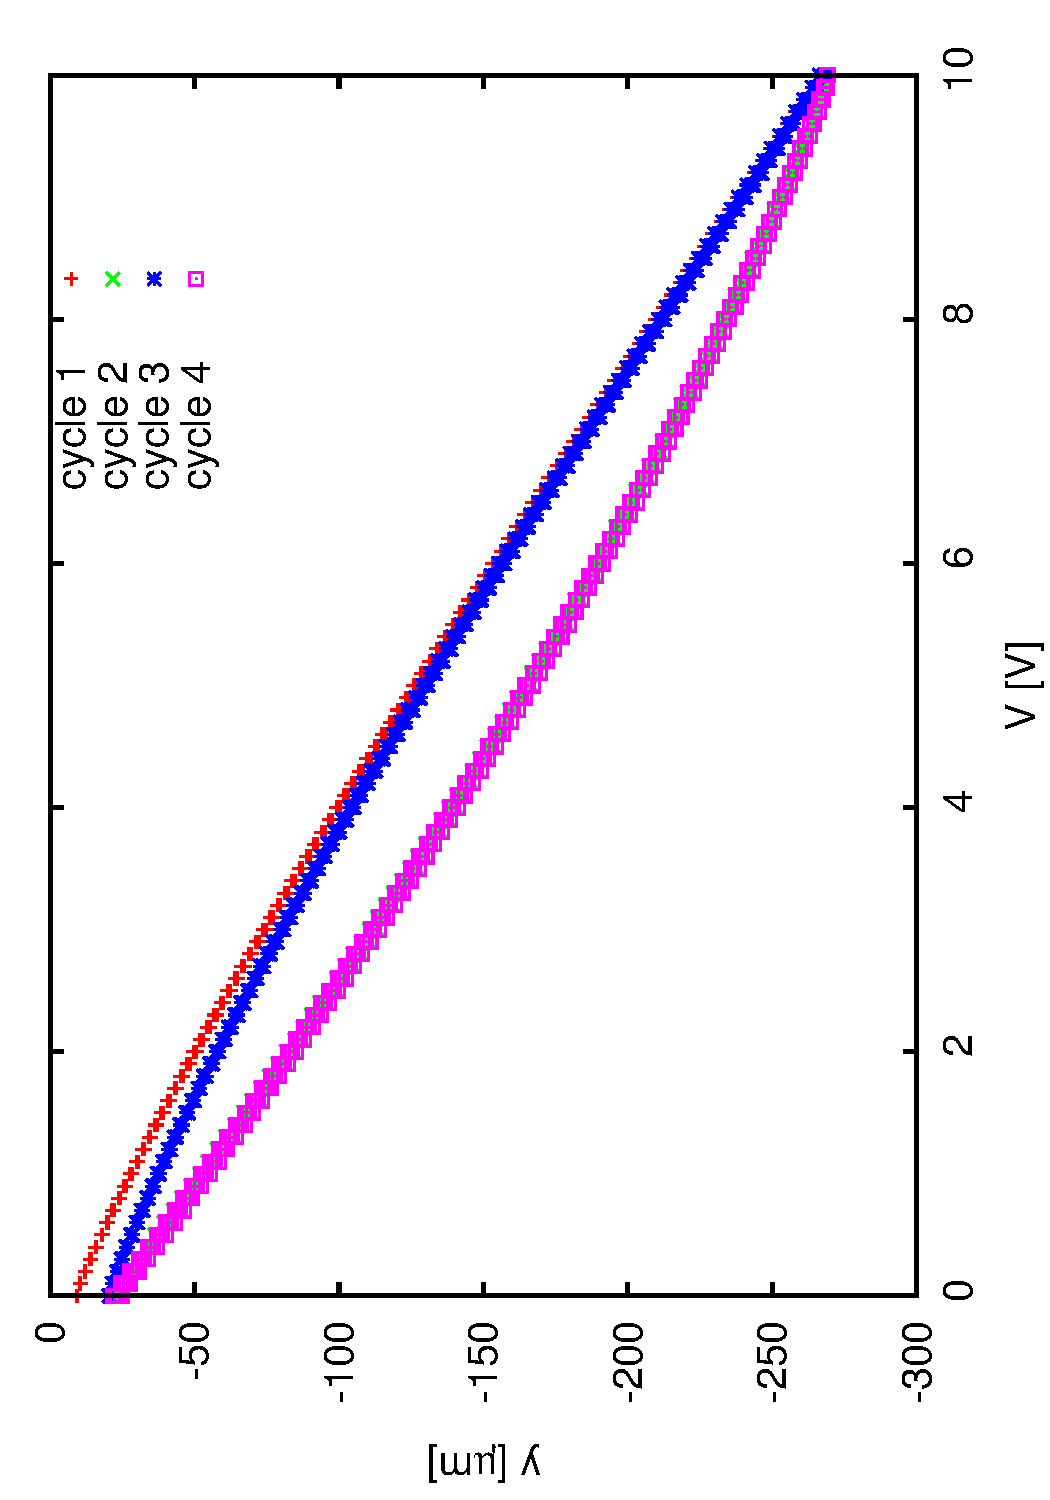
\includegraphics[angle=-90,scale=0.15]{image12.pdf}
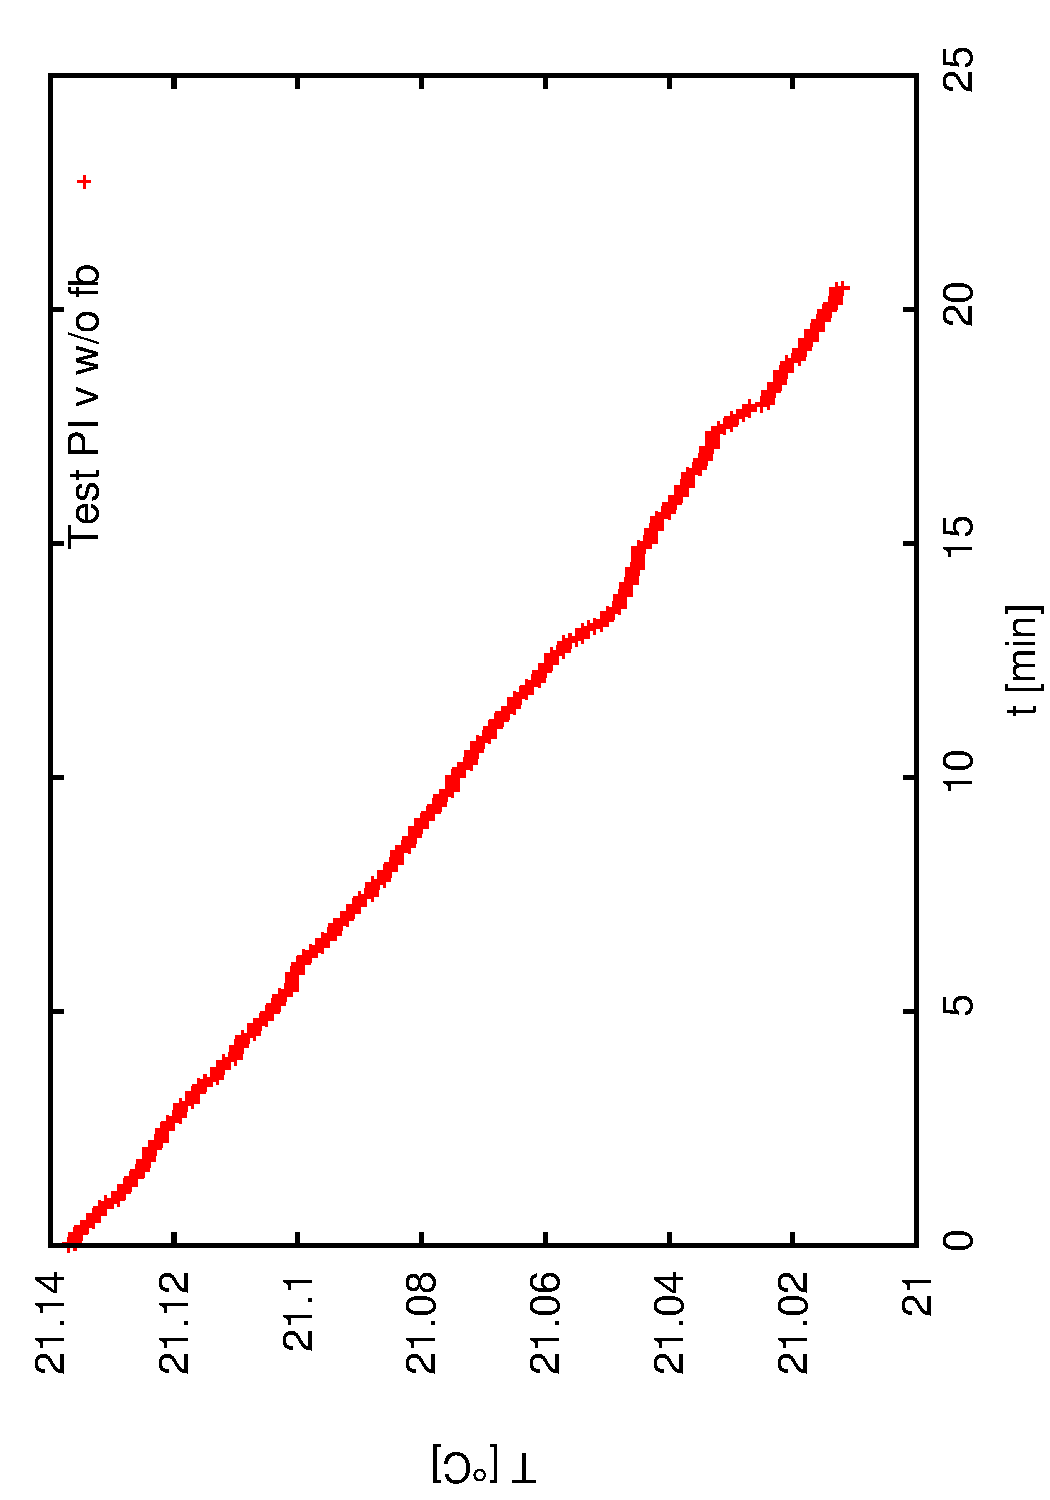
\includegraphics[angle=-90,scale=0.15]{image11a.pdf}\\
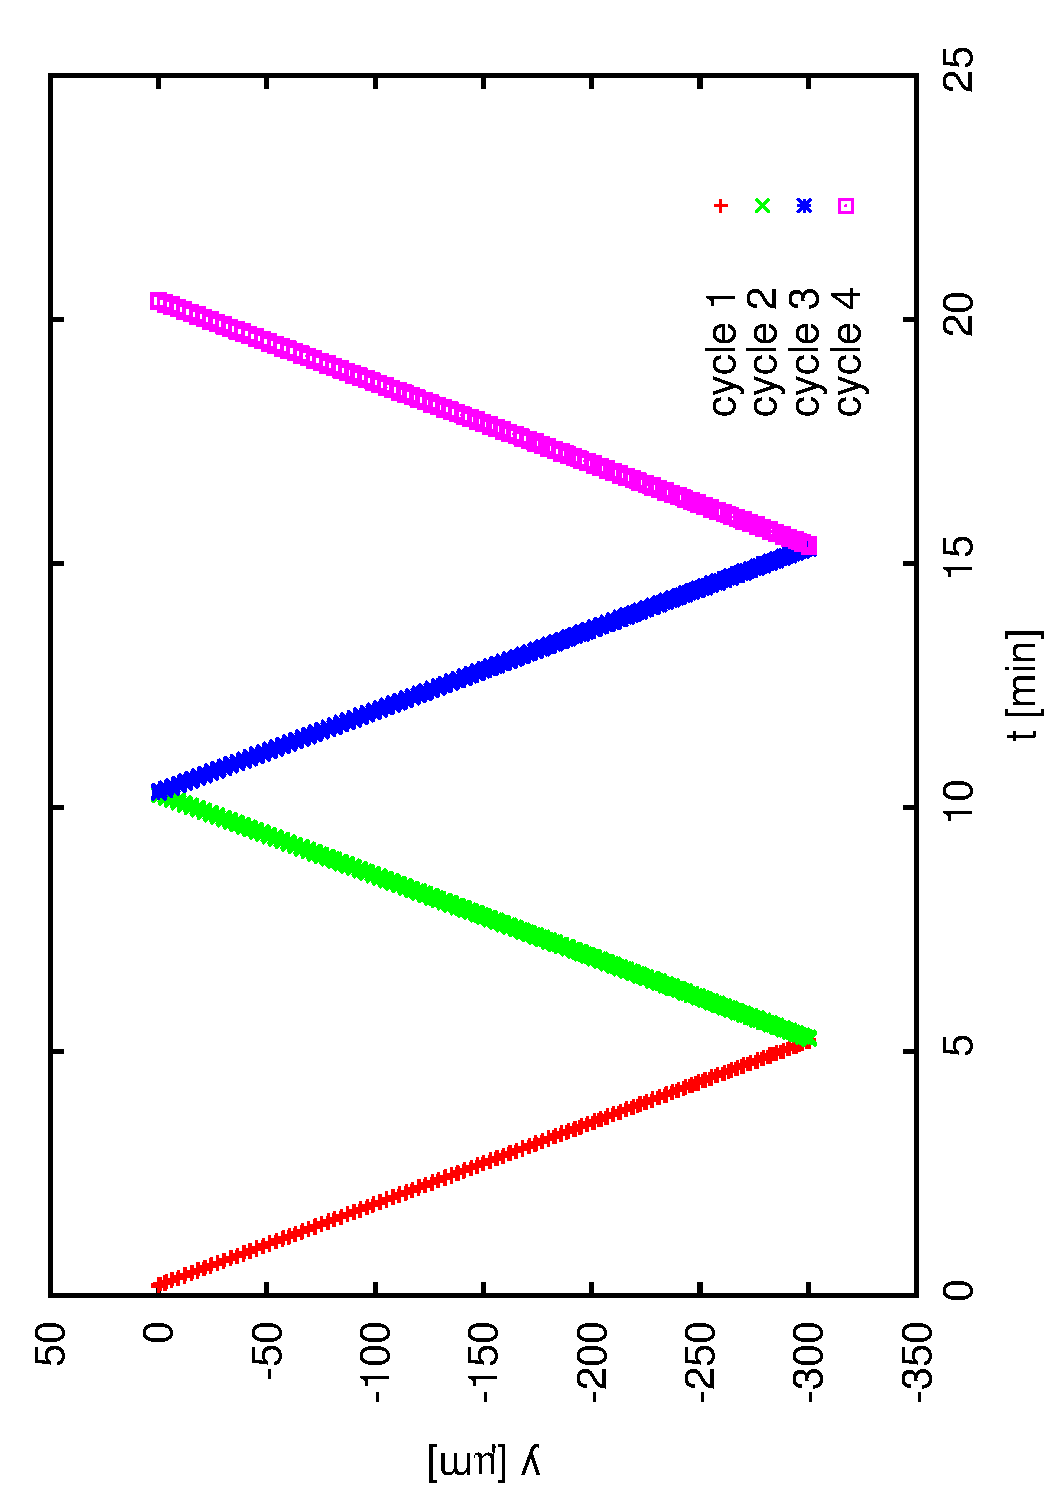
\includegraphics[angle=-90,scale=0.15]{image01.pdf}
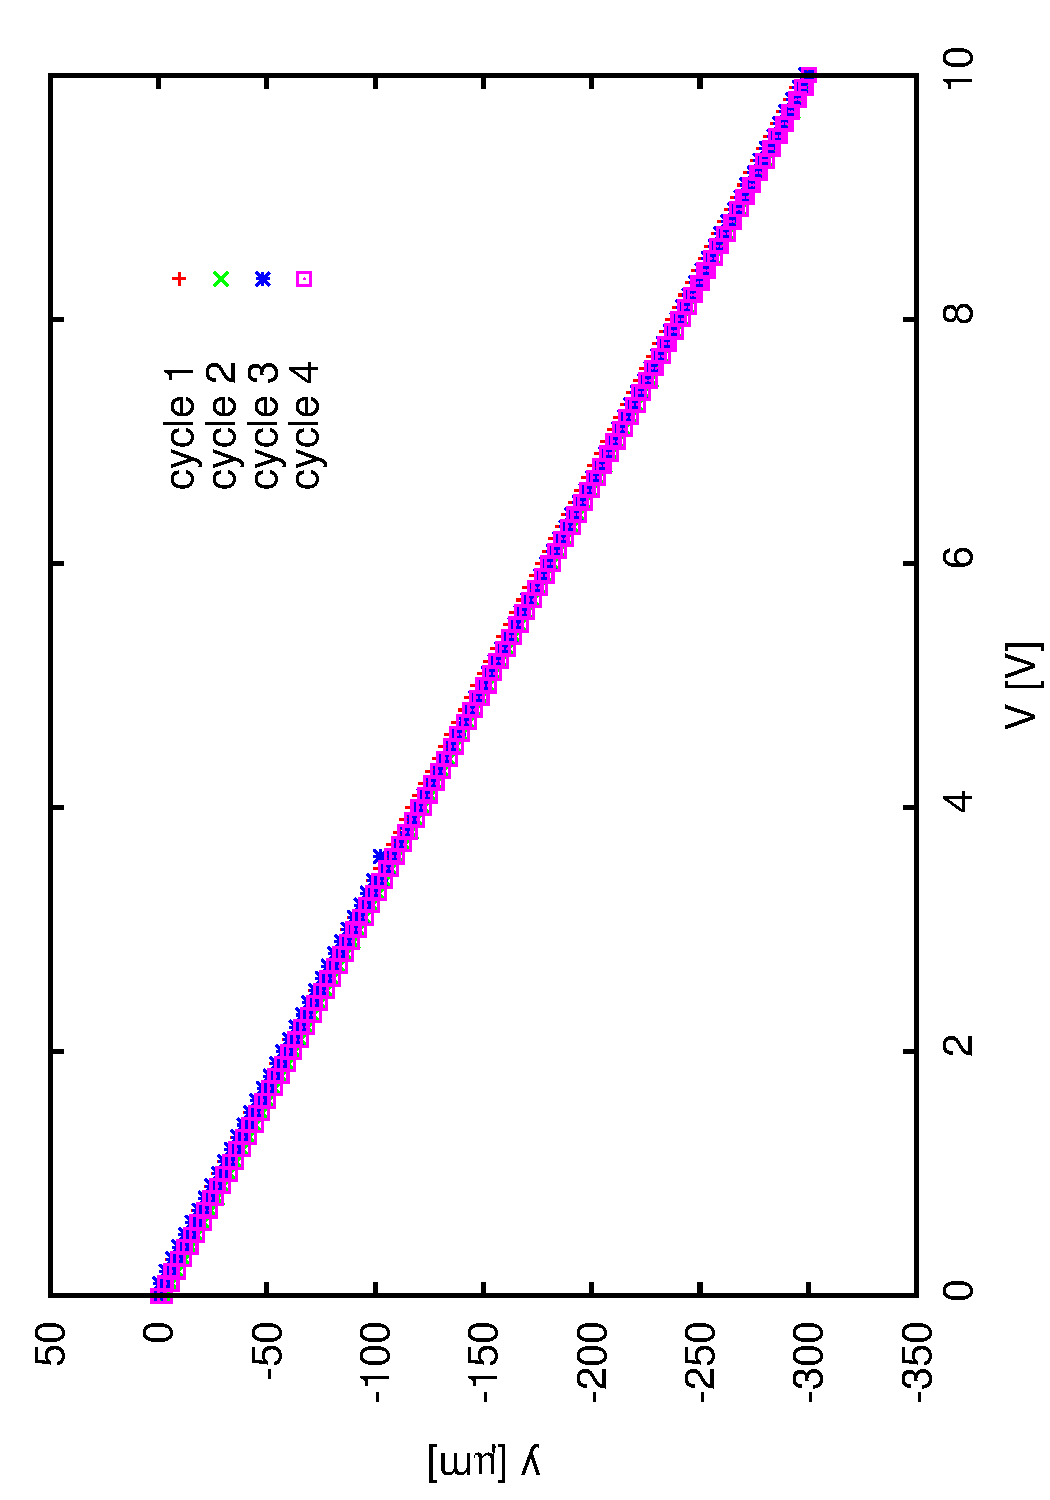
\includegraphics[angle=-90,scale=0.15]{image02.pdf}
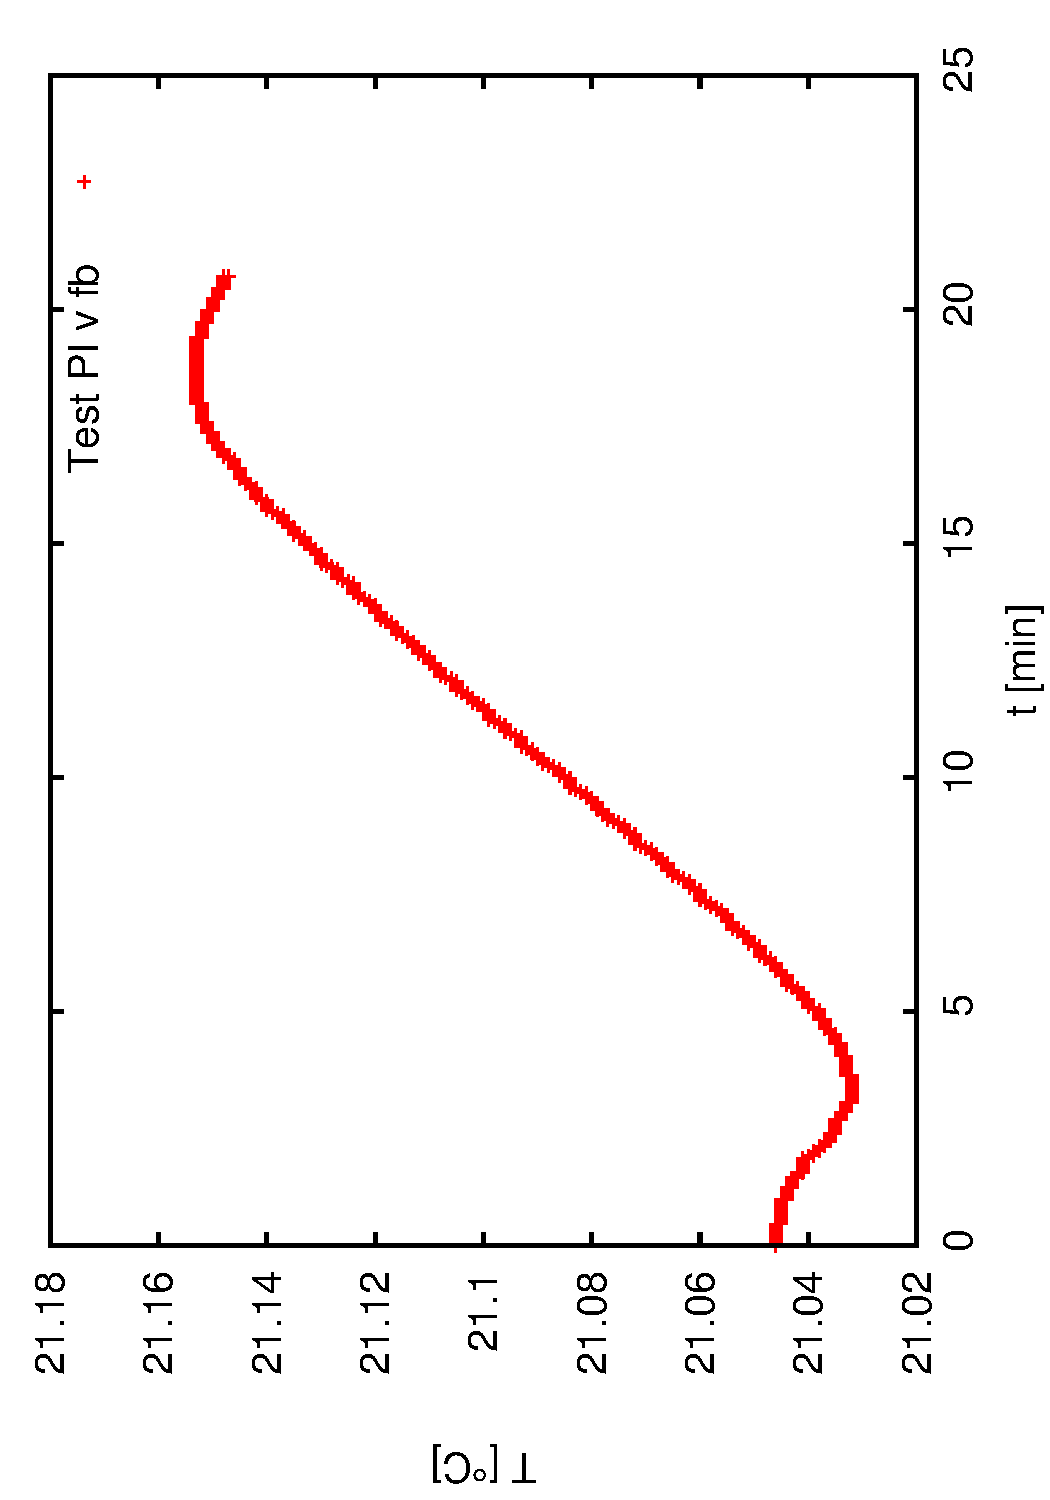
\includegraphics[angle=-90,scale=0.15]{image01a.pdf}\\
 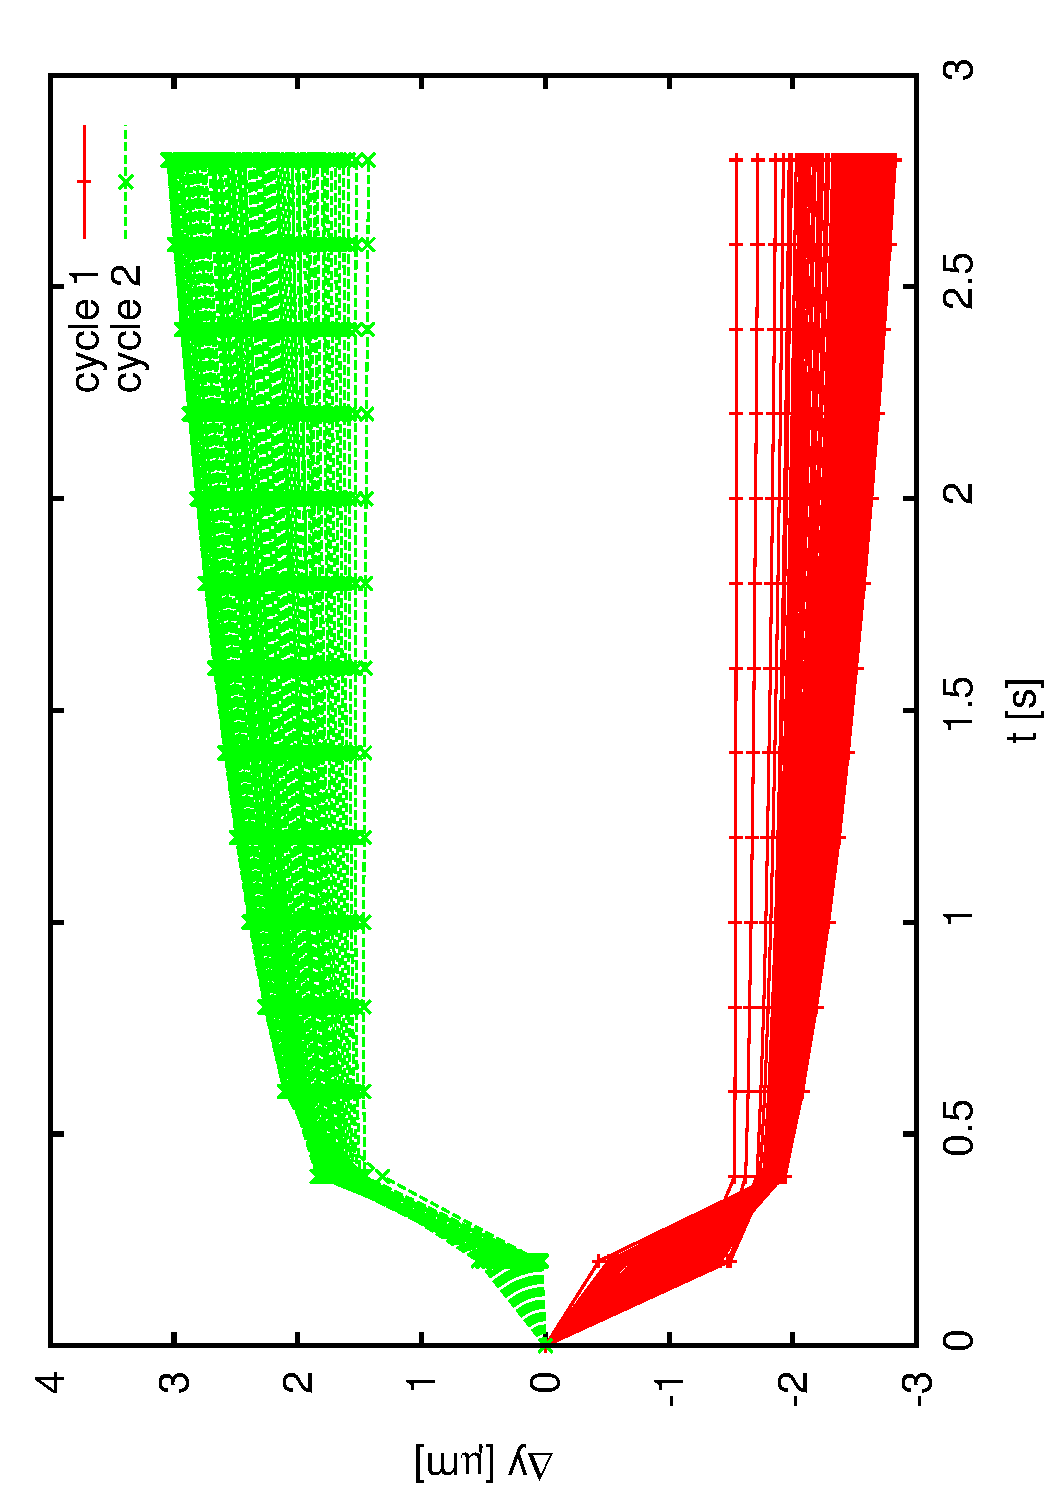
\includegraphics[angle=-90,scale=0.16]{image14.pdf}\\
 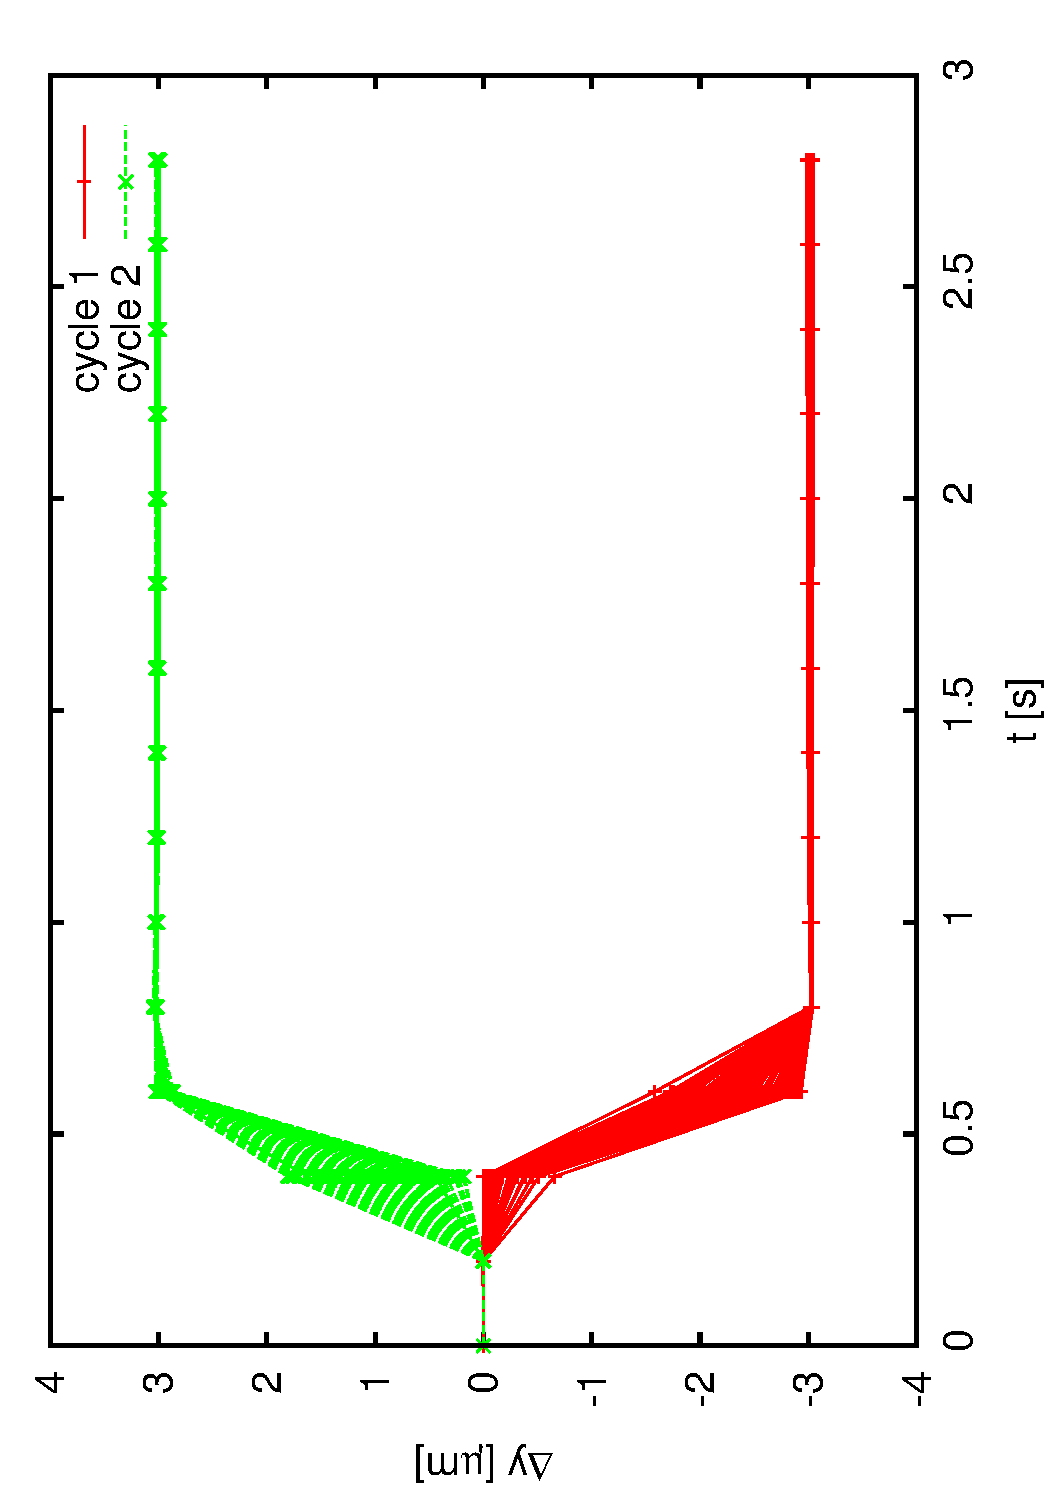
\includegraphics[angle=-90,scale=0.16]{image04.pdf}
 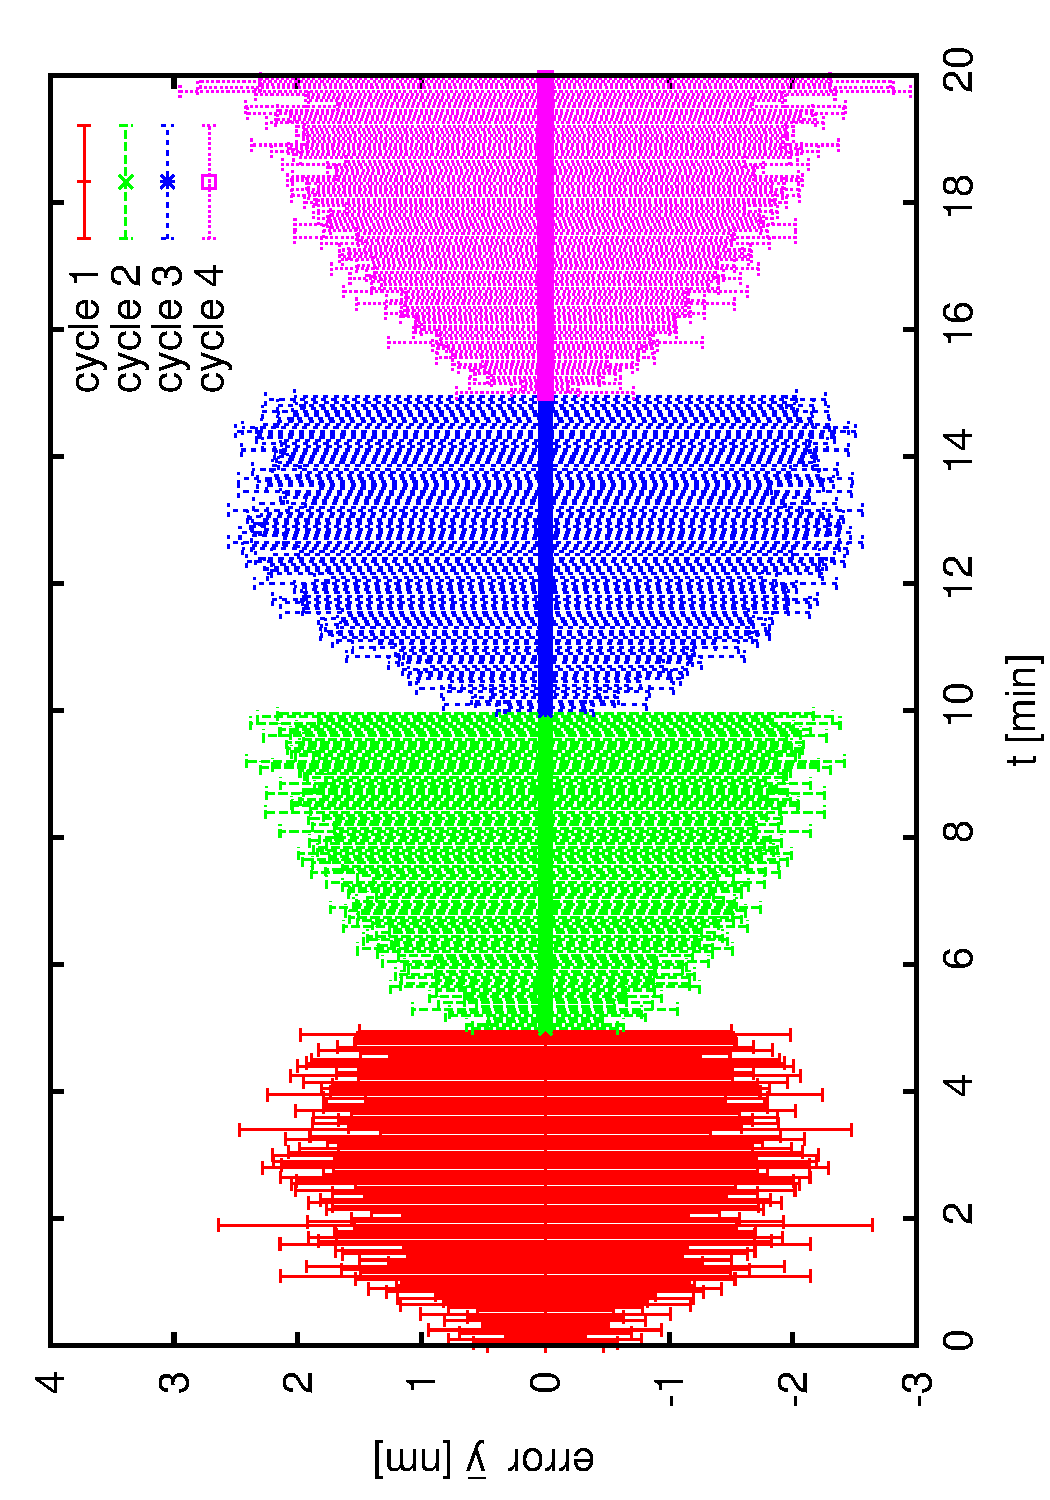
\includegraphics[angle=-90,scale=0.16]{image05c.pdf}\\
 {\tiny Each step is 0.1V (3$\mu$m), sampled 15 times (over 3 s).}\\ 
{\tiny Last 10 points were used to calculate the mean on each step, error over the mean of each step: less than 3nm.}\par
Linearity (with fb)\par
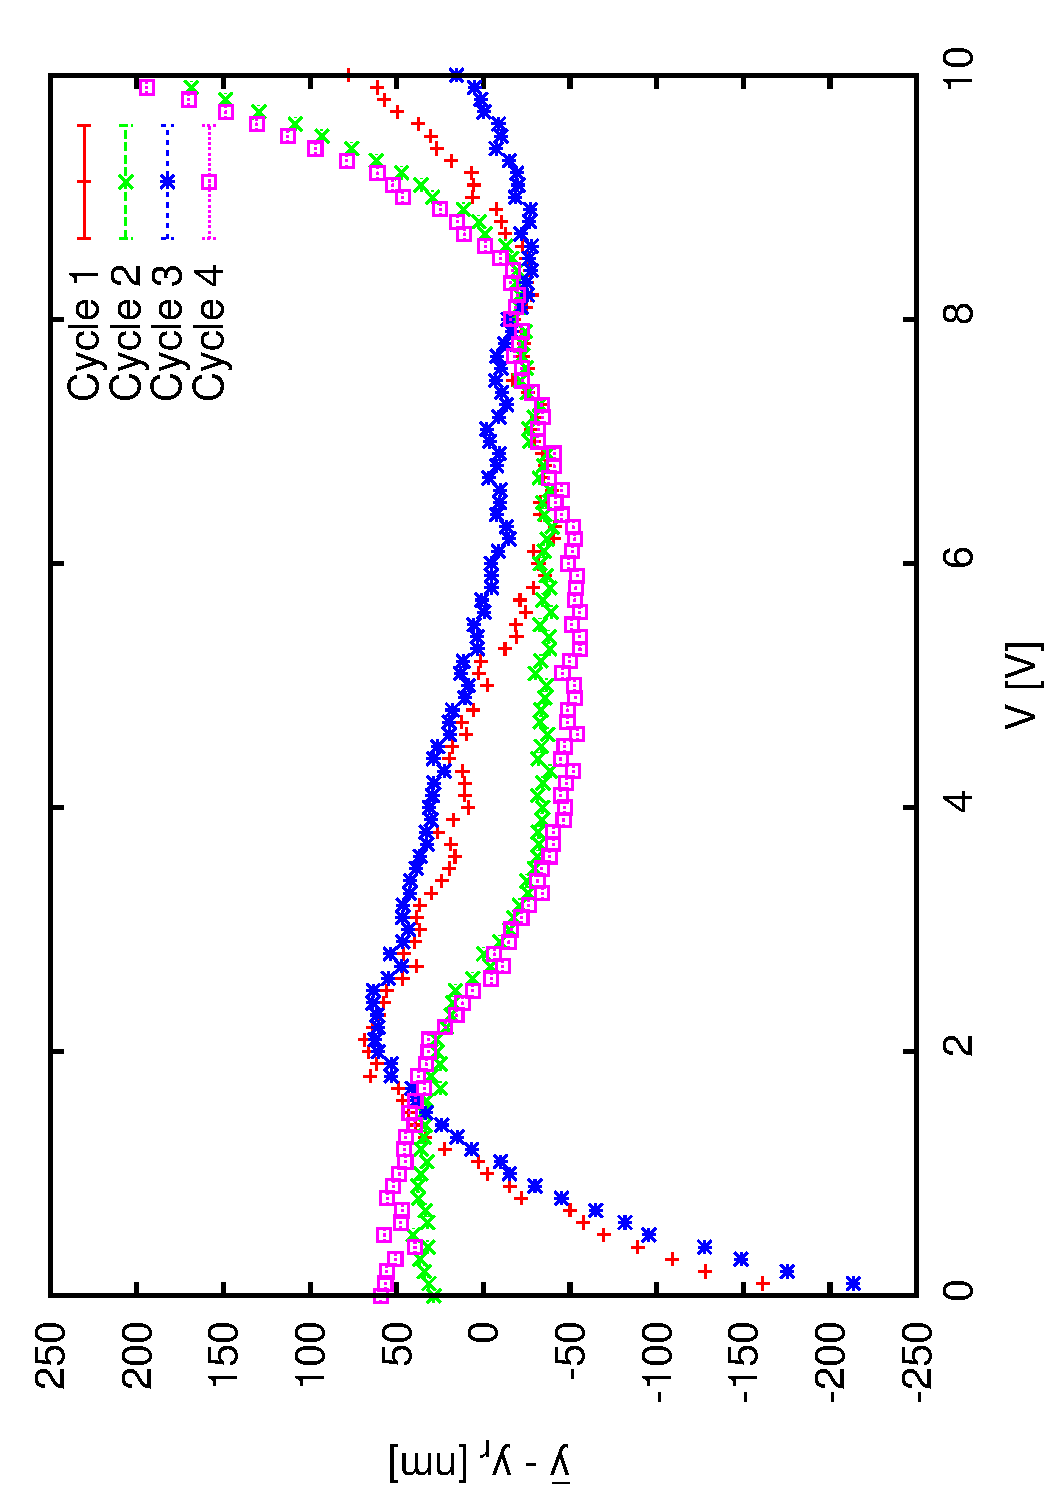
\includegraphics[angle=-90,scale=0.22]{image06e.pdf}
\begin{tabular}[]{|c|c|c|}\hline
 Cycle & Slope[nm/V] & Offset[nm] \\\hline
 {\color{red}1} & $-30011 \pm 1$& $-191\pm9$\\
{\color{green}2} & $-29997 \pm 1$& $-204\pm9$ \\
{\color{blue}3} & $-29982 \pm 2$& $-502\pm9$\\
{\color{magenta}4} & $-30018 \pm2$ & $84\pm11$\\\hline
\end{tabular}\\Slope mean = $30002\pm7$\\Previous result by Frédéric Bogard showed $\sim$120nm/0.1$^\circ$C (if no delay)\\
%$\rightarrow\pm4\times10^{-4}$ when $\Delta$T = 0.1$^\circ$C
 %Offsets and slope variations might come from temperature deviation.
 
Minimum step and speed (with fb)
Each step is 0.1V (3$\mu$m), sampled 15 times (over 3 s)\\
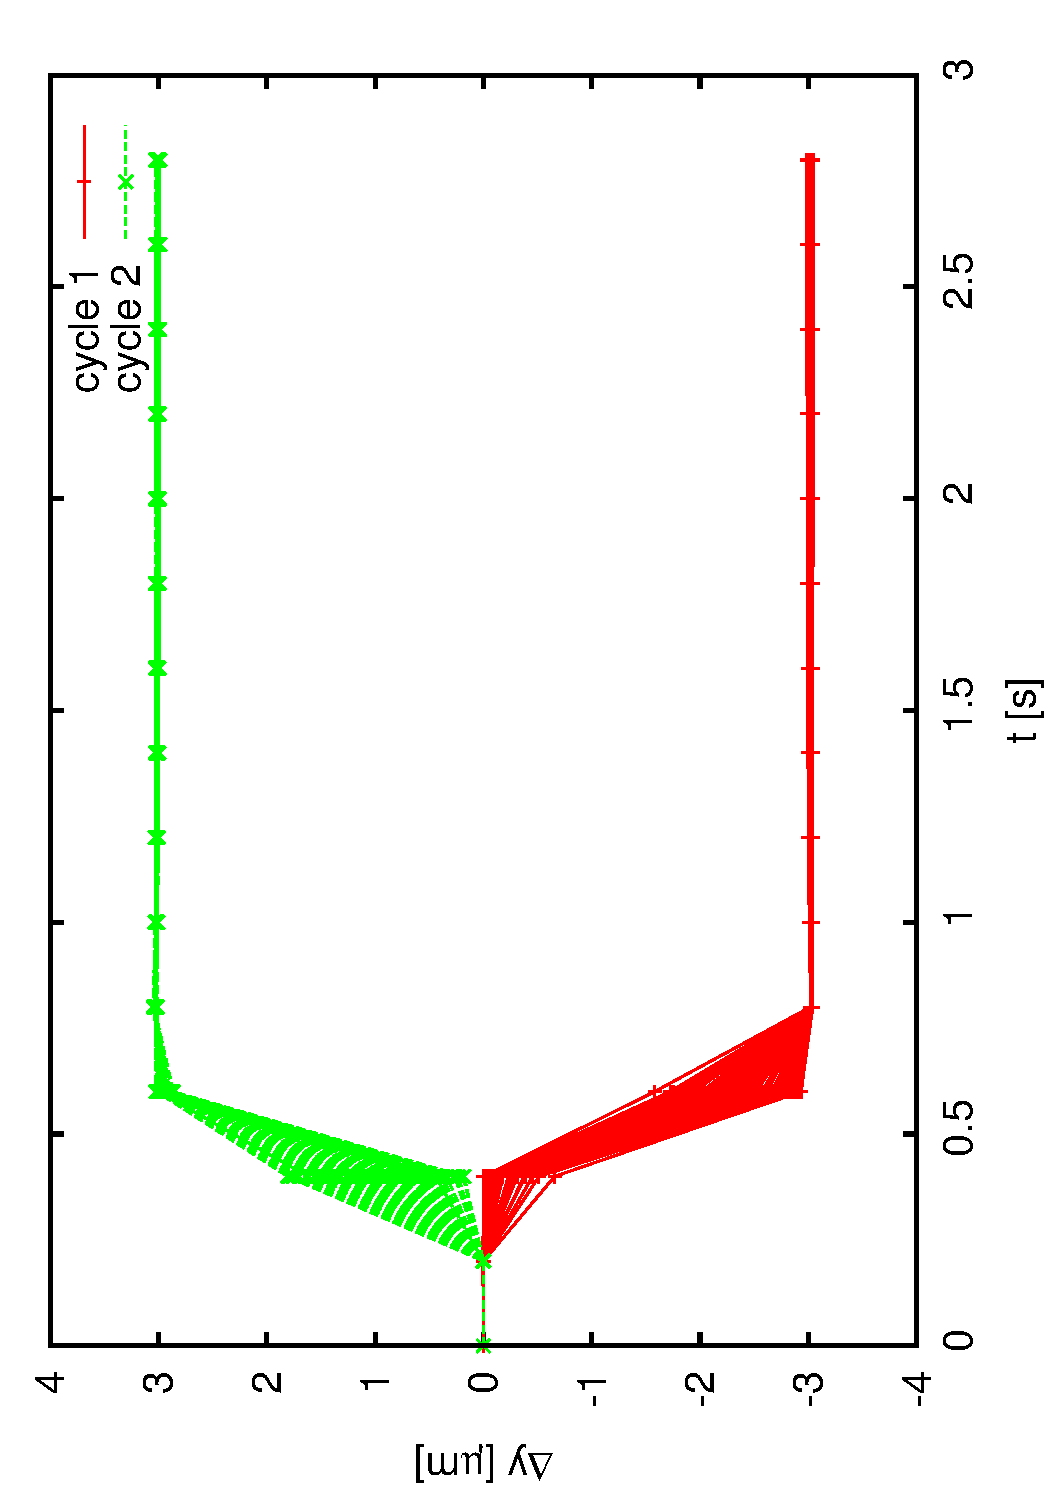
\includegraphics[angle=-90,scale=0.22]{image04.pdf}
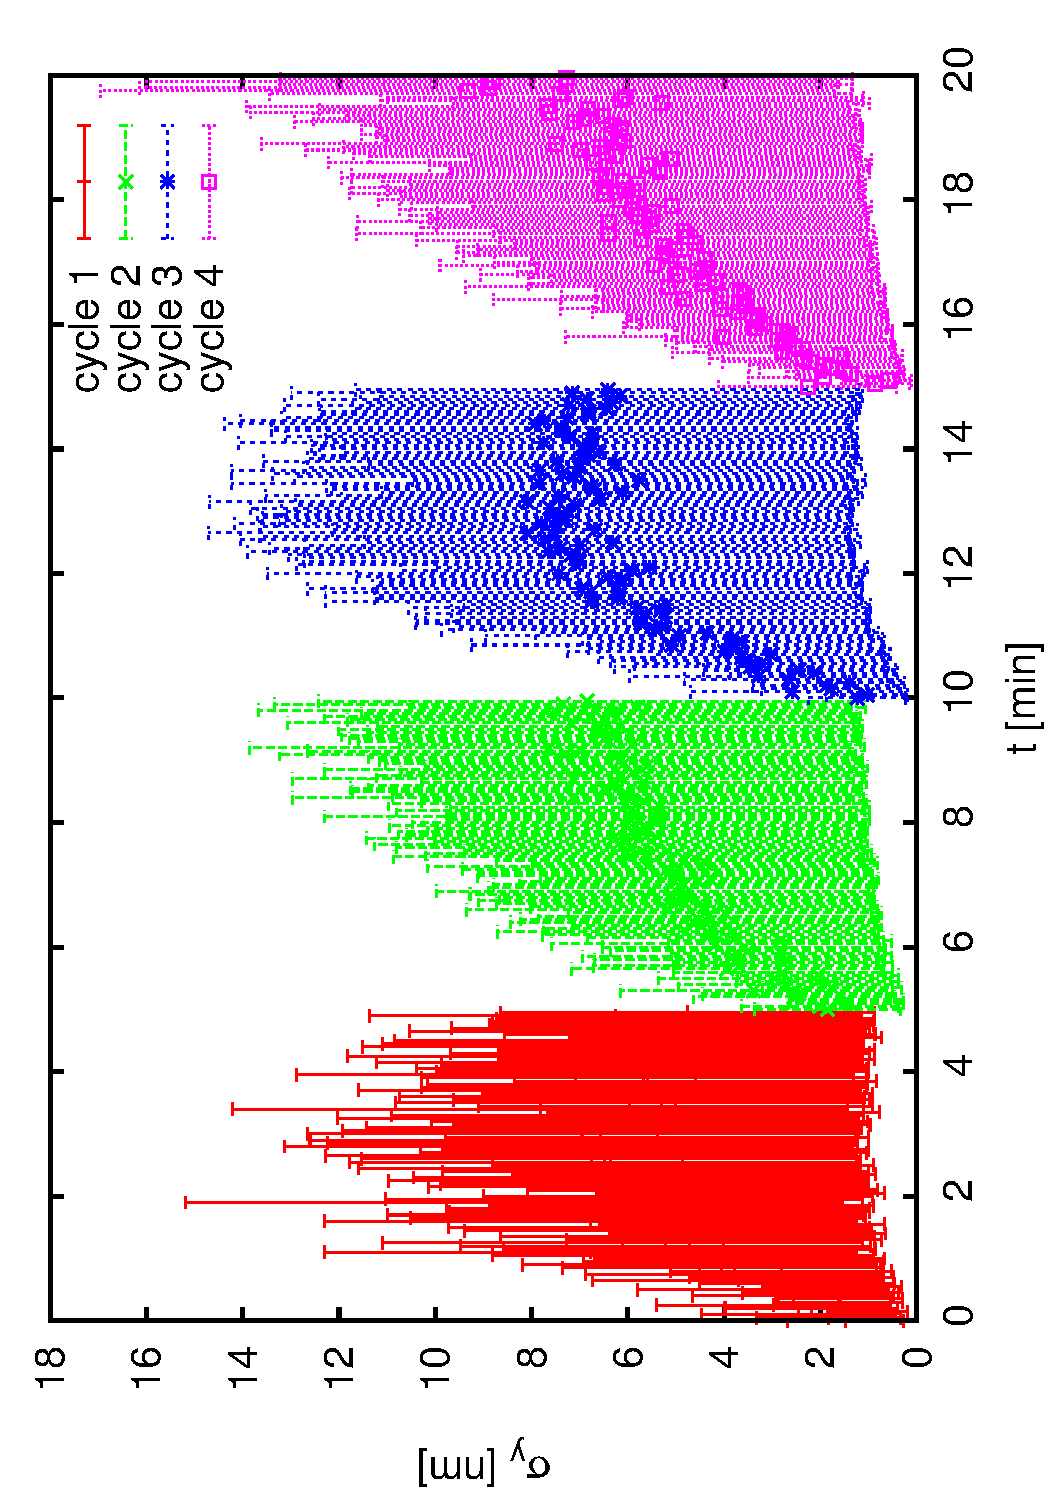
\includegraphics[angle=-90,scale=0.22]{image05.pdf}\\
system can respond at 3$\mu$m$/$s\\
Minumum current step is 18nm.

\subsubsection{Cedrat without and with feedback}
Four cycles (two going up, two going down), range (-1$\sim$7V, 0$\sim$250$\mu$m)\par
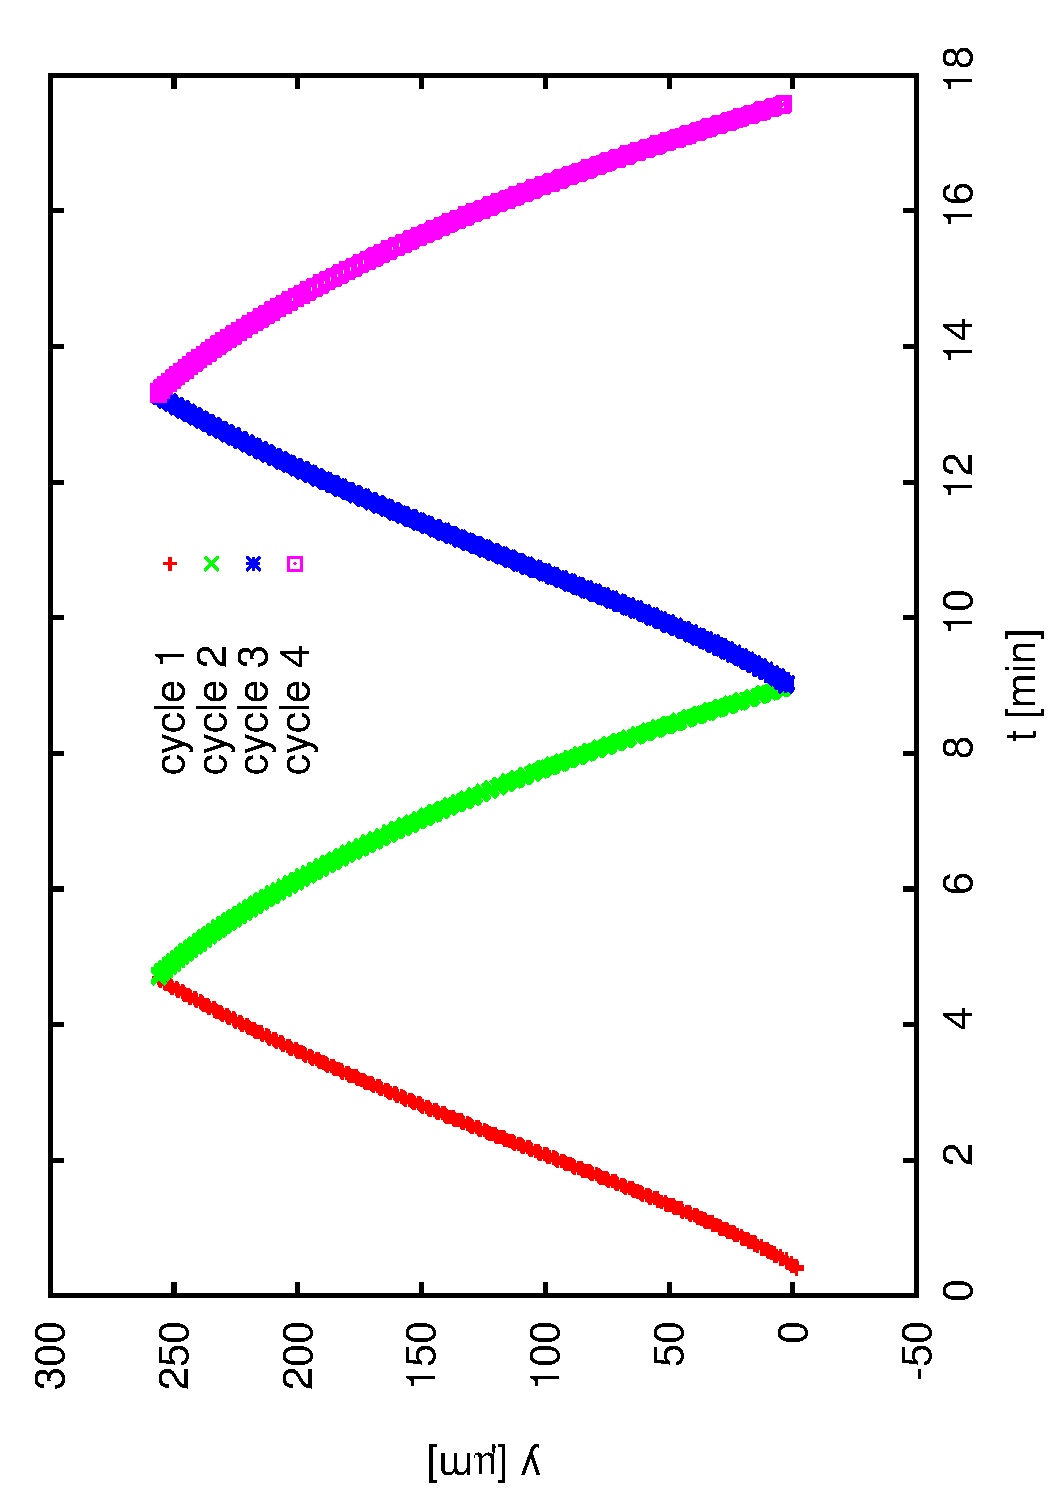
\includegraphics[angle=-90,scale=0.15]{image31.pdf}
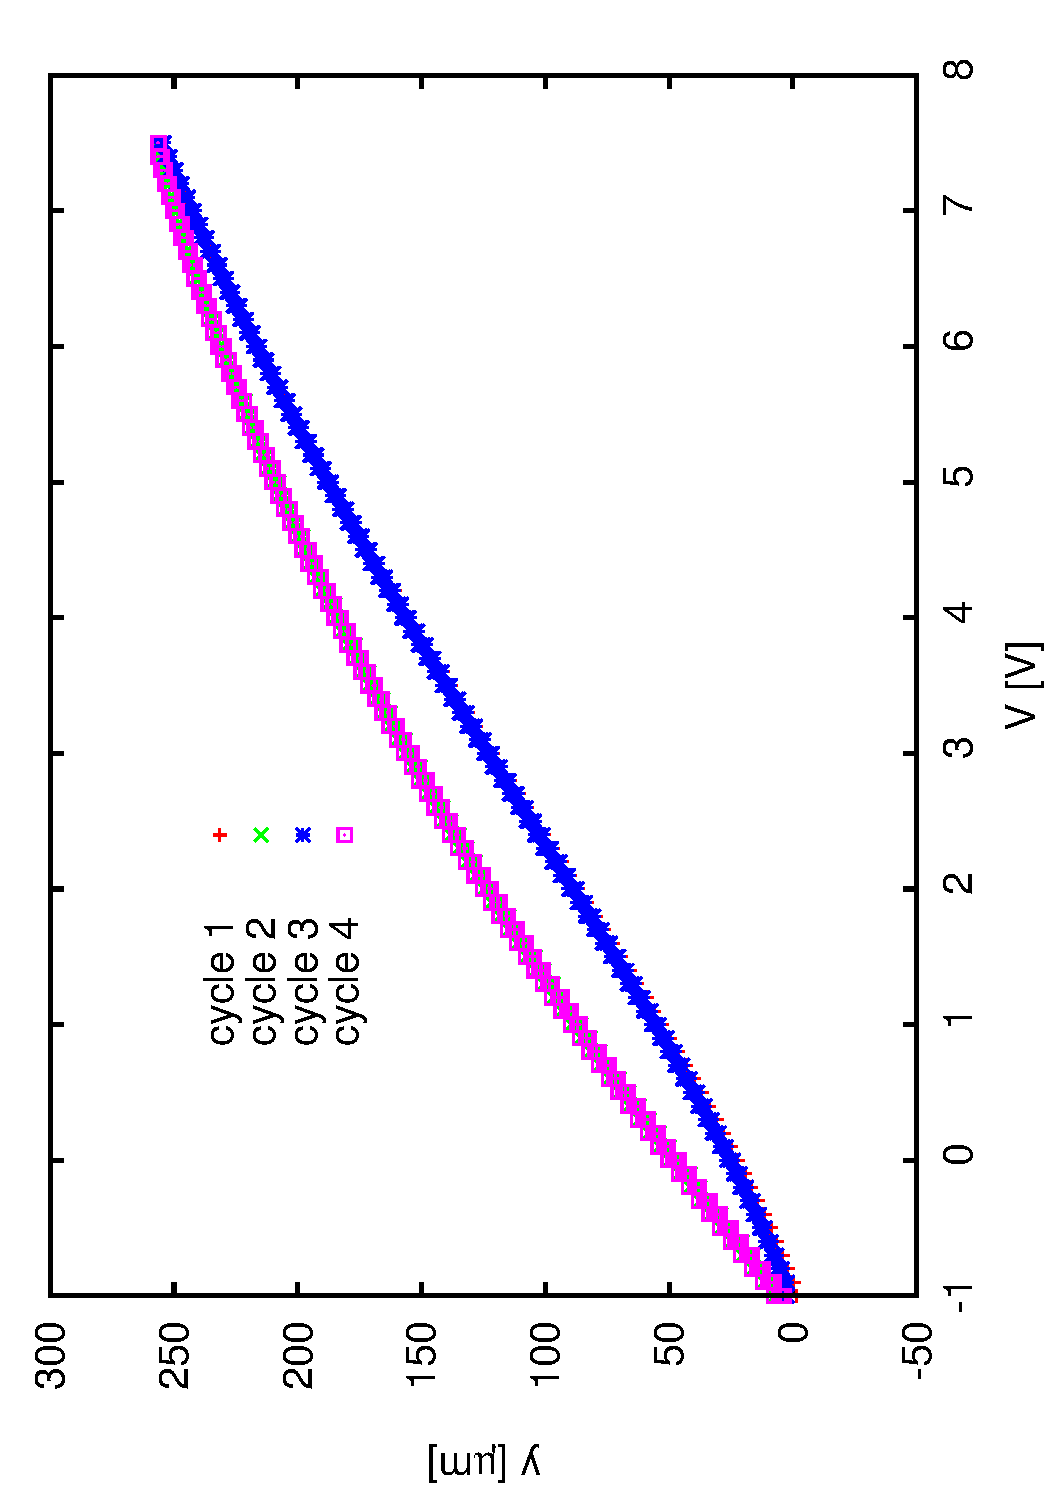
\includegraphics[angle=-90,scale=0.15]{image32.pdf}
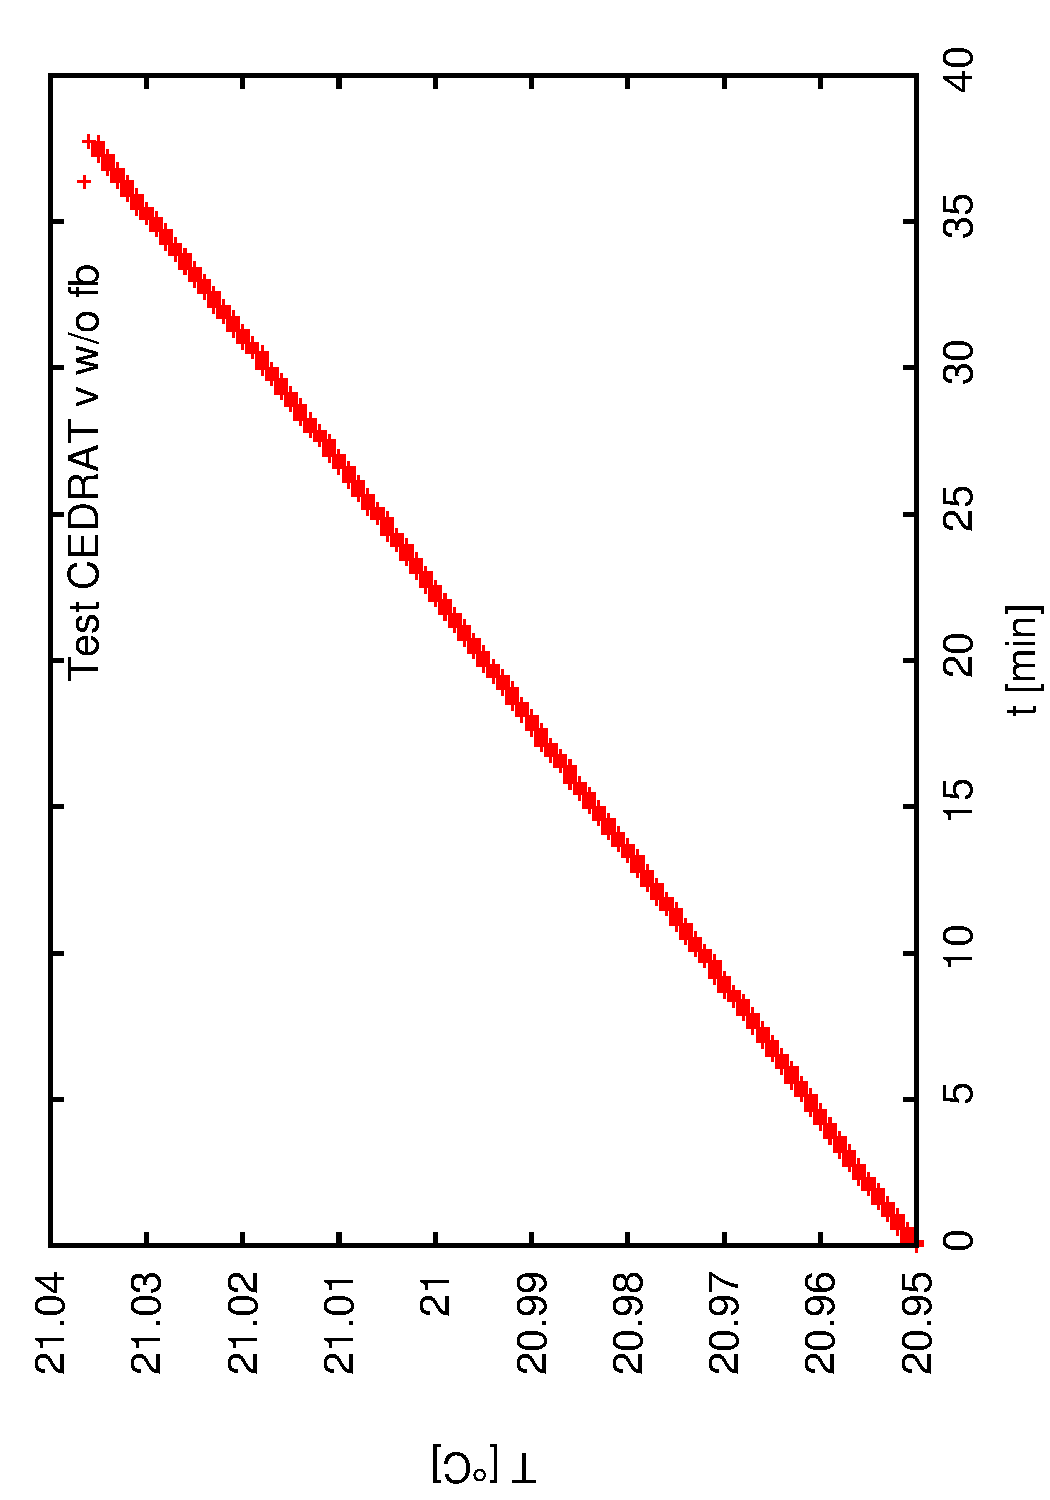
\includegraphics[angle=-90,scale=0.15]{image31a.pdf}\\
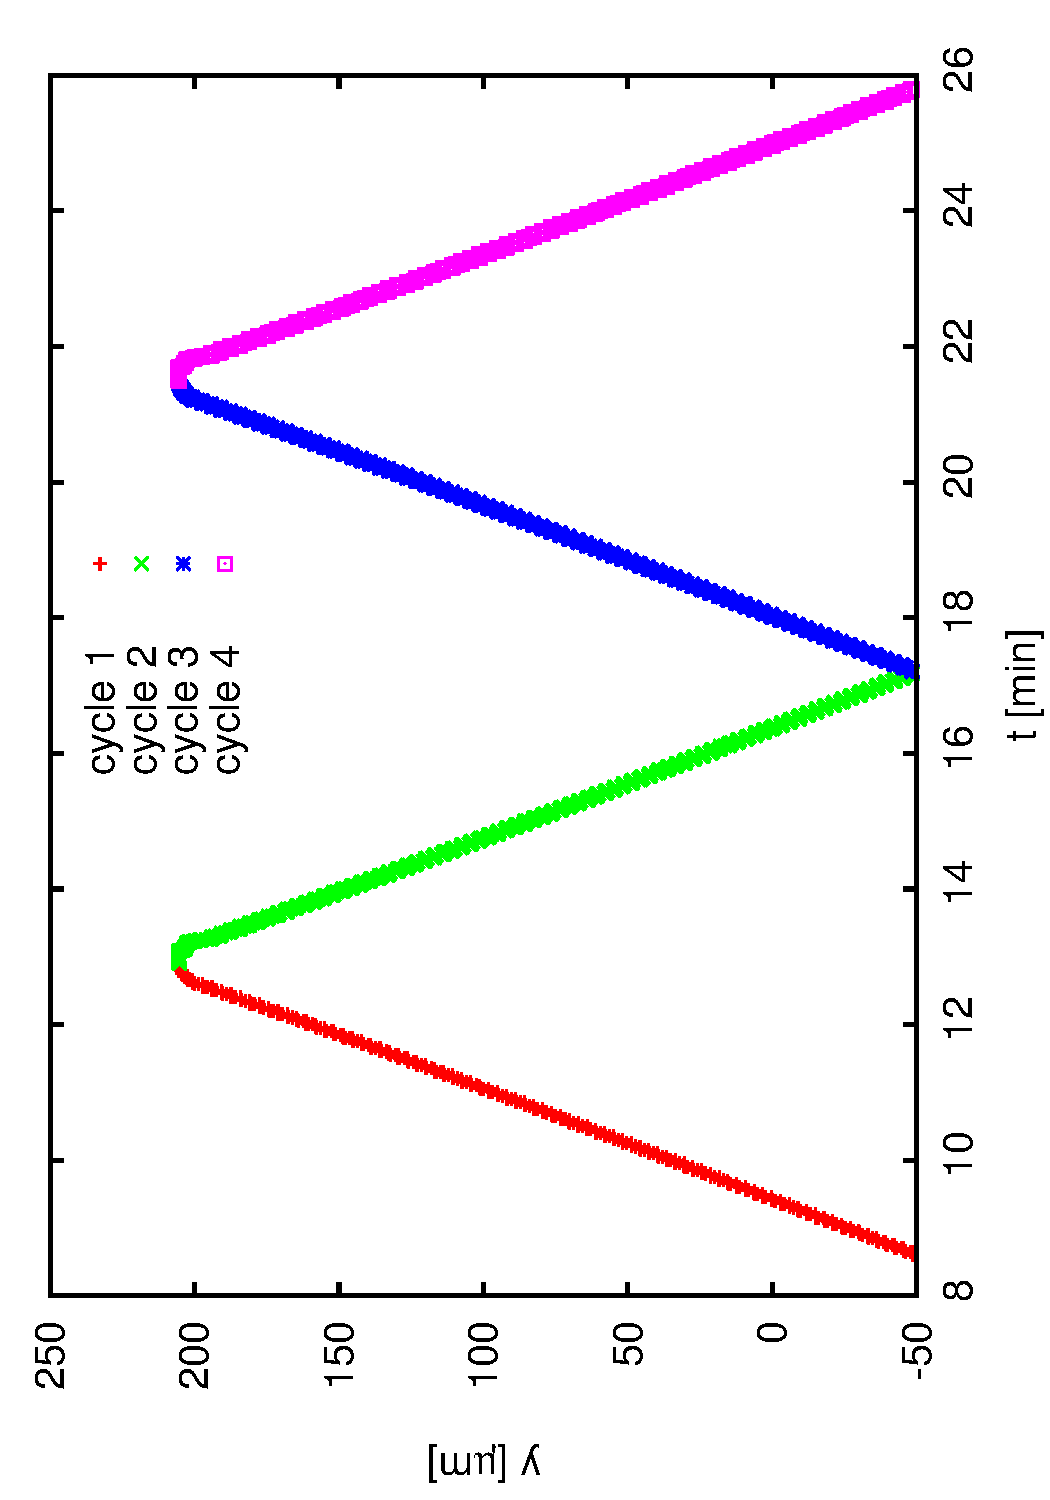
\includegraphics[angle=-90,scale=0.15]{image21.pdf}
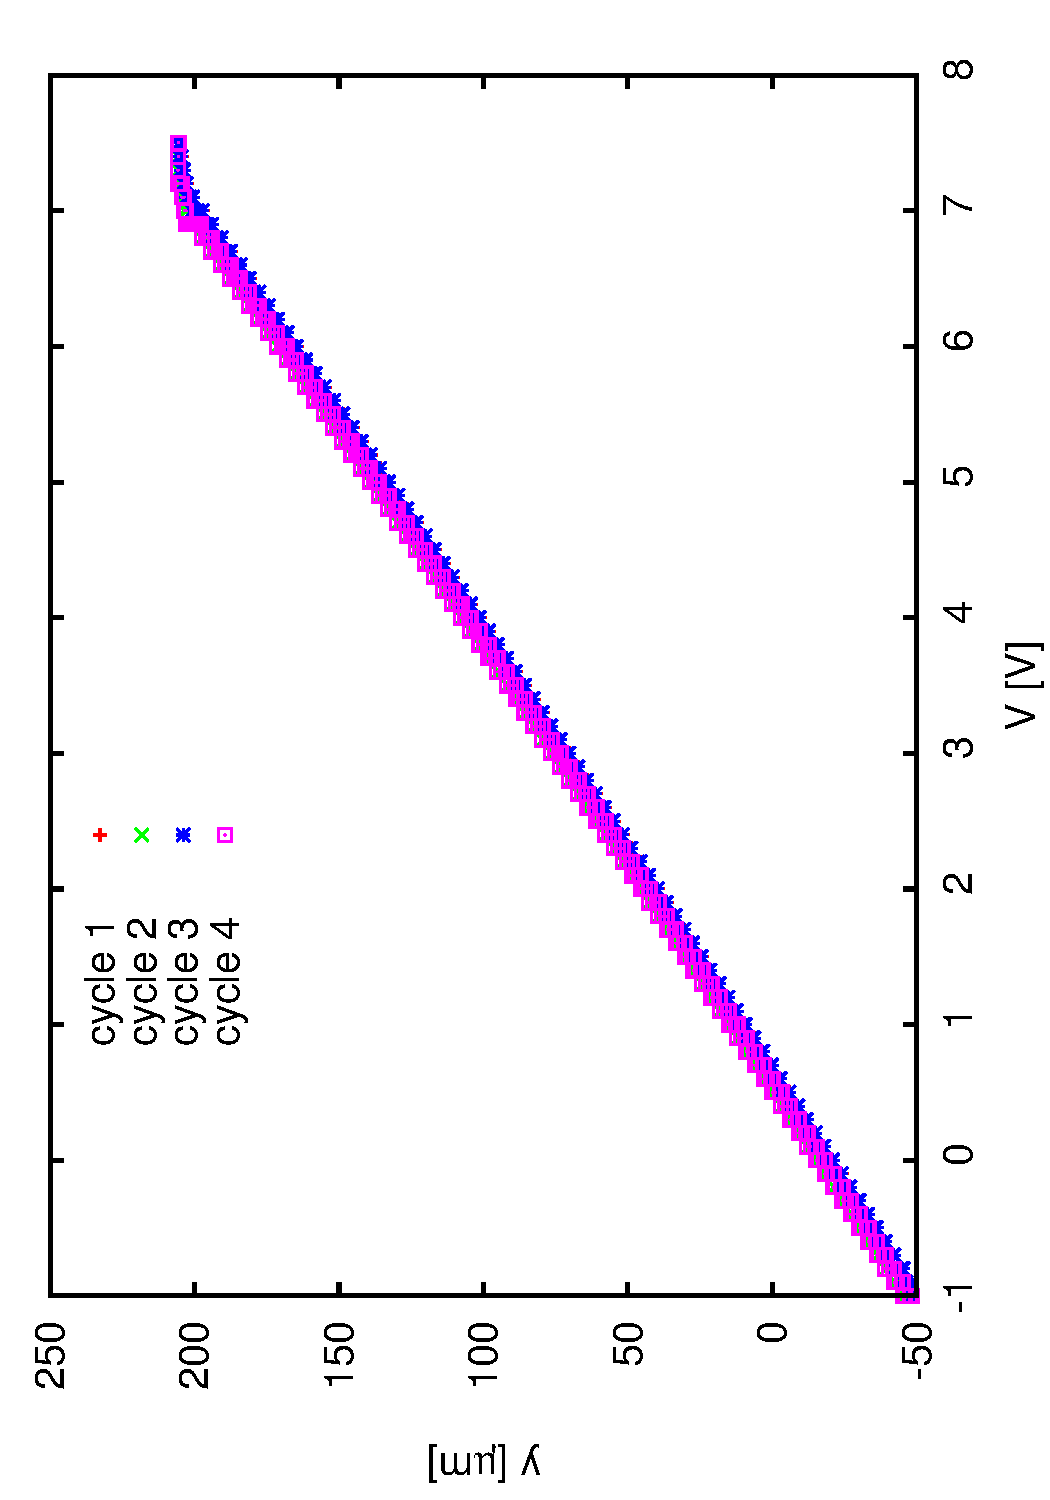
\includegraphics[angle=-90,scale=0.15]{image22.pdf}
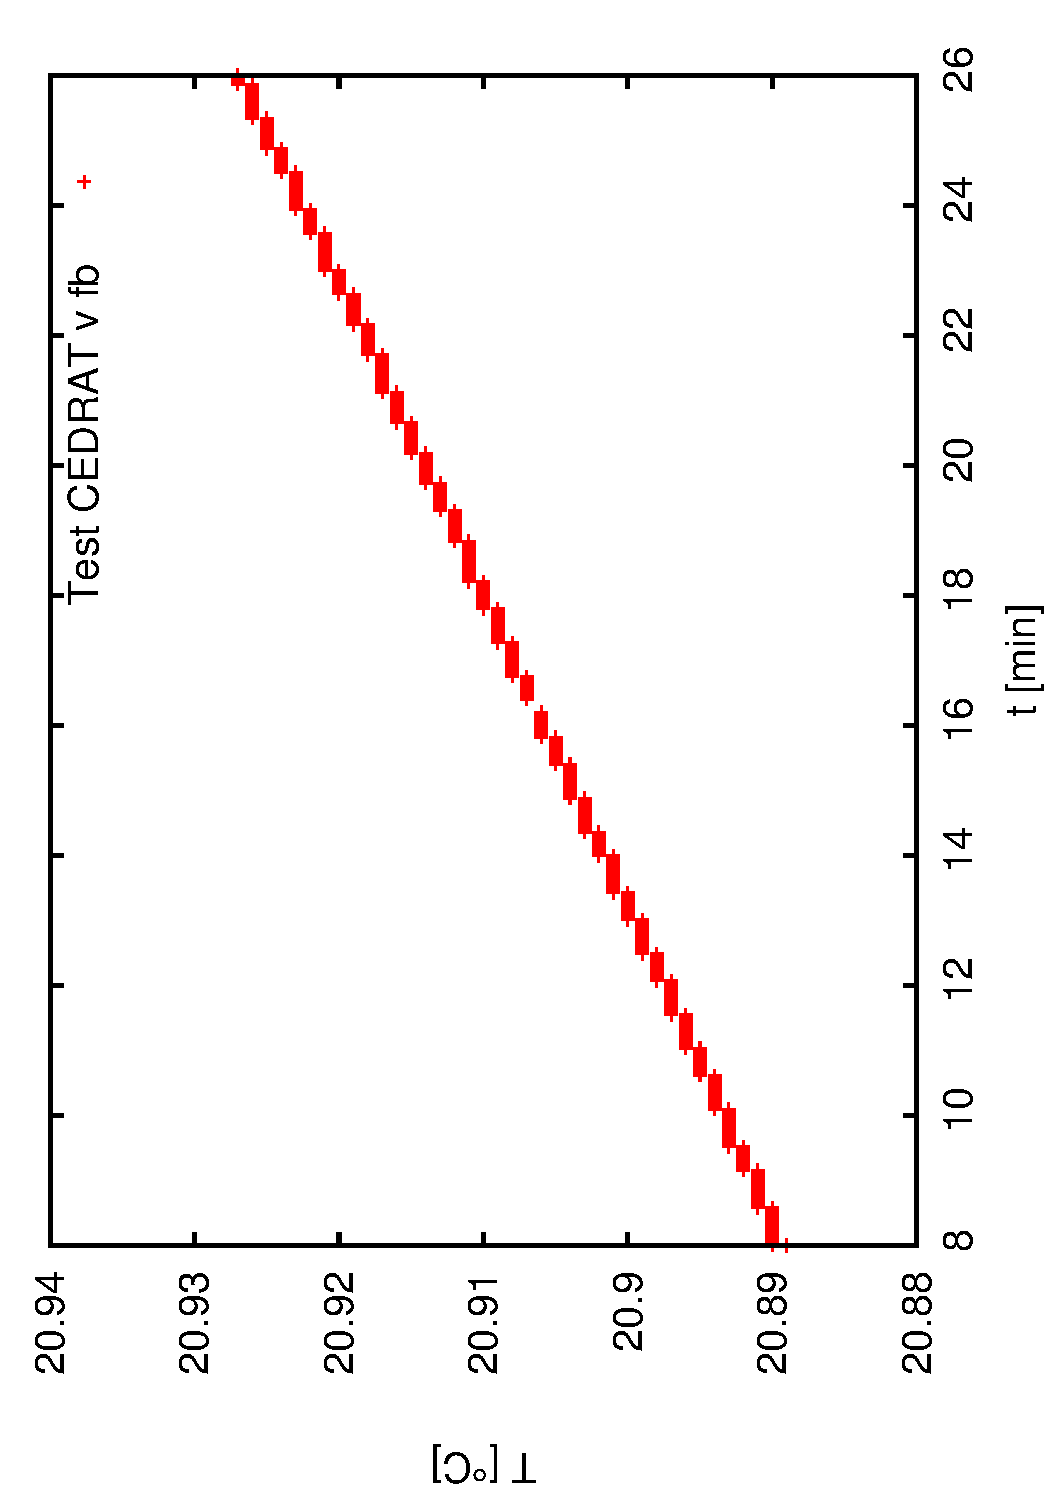
\includegraphics[angle=-90,scale=0.15]{image21a.pdf}\par
 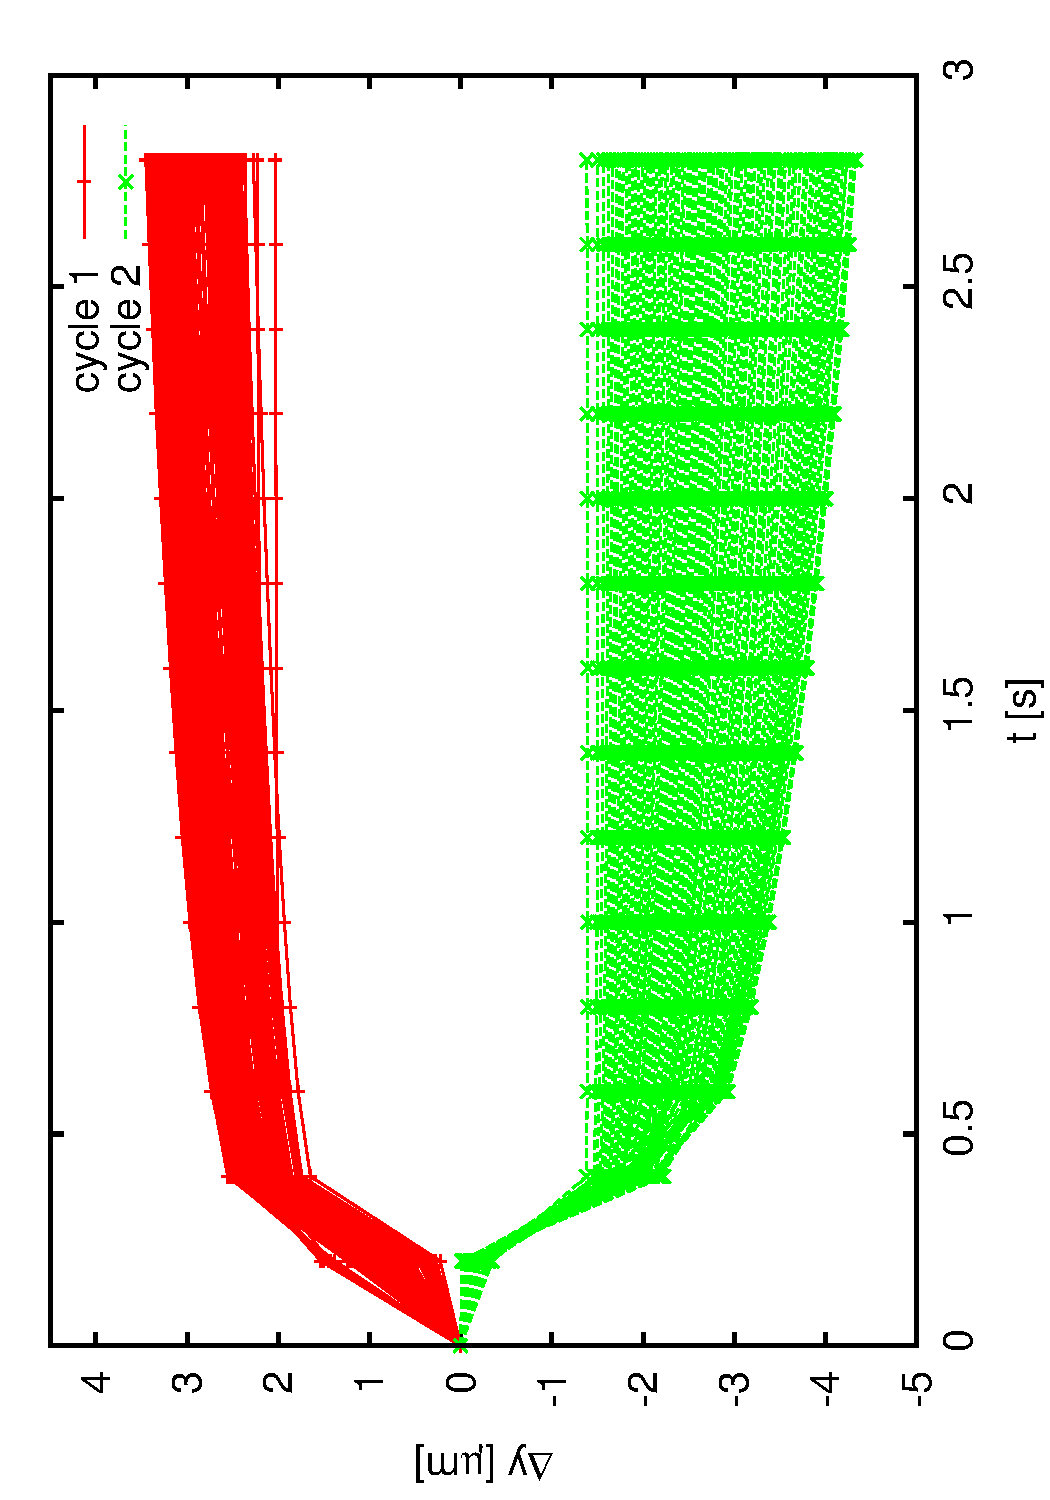
\includegraphics[angle=-90,scale=0.16]{image34.pdf}\\
 \includegraphics[angle=-90,scale=0.16]{image24.pdf}
 \includegraphics[angle=-90,scale=0.16]{image25c.pdf}\\
{\tiny Each step is 0.1V ($\sim3.125\mu$m), sampled 15 times (over 3 s).}
{\tiny Last 10 points were used to calculate the mean on each step\\Error over the mean of each step: less than 15nm.}\par

Linearity (with fb)
\includegraphics[angle=-90,scale=0.22]{image26e.pdf}
\begin{tabular}[]{|c|c|c|}\hline
 Cycle & Slope[nm/V] & Offset[nm] \\\hline
 {\color{red}1} & $30988 \pm 41$& $-18670\pm154$\\
{\color{green}2} & $31039 \pm 42$& $-19092\pm154$ \\
{\color{blue}3} & $30993\pm 41$& $-18547\pm156$\\
{\color{magenta}4} & $31040 \pm42$ & $-18935\pm154$\\\hline
\end{tabular}\\Slope mean = $31015\pm12$($\pm42$)\\Unknown temperature effect\\
%$\rightarrow\pm4\times10^{-4}$ when $\Delta$T = 0.1$^\circ$C
 %Offsets and slope variations might come from temperature deviation.
Minimum step and speed (with fb)
\includegraphics[angle=-90,scale=0.22]{image24.pdf}
\includegraphics[angle=-90,scale=0.22]{image25.pdf}\\
System can respond at 3$\mu$m$/$s\\
Minimum current step is 80nm.

\subsubsection{From Gauges}
Lateral fixed
 \includegraphics[angle=-90,scale=0.20]{image_ai_01.pdf}
 \includegraphics[angle=-90,scale=0.20]{image_ai_02.pdf}\\
Verticals fixed
 \includegraphics[angle=-90,scale=0.20]{image_ai_03.pdf}
 \includegraphics[angle=-90,scale=0.20]{image_ai_04.pdf}\\ 

 
 \subsubsection{Summary}
 \;{\tiny Four cycles,range (0$\sim$10V, 0$\sim$300$\mu$m)}\\
\textbf{PI without fb}\hspace*{4cm}\textbf{PI with  fb}\par
\includegraphics[angle=-90,scale=0.10]{image12.pdf}\hspace*{2cm}
\includegraphics[angle=-90,scale=0.10]{image02.pdf}
\includegraphics[angle=-90,scale=0.14]{image06e.pdf}\par
Lateral fixed\hspace{1.8cm}(fb)\hspace{3.0cm}(no fb)\par
 \hspace*{2cm}\includegraphics[angle=-90,scale=0.15]{image_ai_01.pdf}
 \includegraphics[angle=-90,scale=0.15]{image_ai_02.pdf}\\
 Vertical fixed\hspace{1.6cm}(fb)\hspace{3.0cm}(no fb)\\
 \hspace*{2cm}\includegraphics[angle=-90,scale=0.15]{image_ai_03.pdf}
 \includegraphics[angle=-90,scale=0.15]{image_ai_04.pdf}\\
{\tiny Four cycles, range (-1$\sim$7V, 0$\sim$250$\mu$m)}\\
\textbf{Cedrat without fb}\hspace*{3.2cm}\textbf{Cedrat with  fb}\par
\includegraphics[angle=-90,scale=0.10]{image32.pdf}\hspace*{2cm}
\includegraphics[angle=-90,scale=0.10]{image22.pdf}
\includegraphics[angle=-90,scale=0.14]{image26e.pdf}\par
Lateral fixed\hspace{1.8cm}(fb)\hspace{3.0cm}(no fb)\par
 \hspace*{2cm}\includegraphics[angle=-90,scale=0.15]{image_ai_11.pdf}
 \includegraphics[angle=-90,scale=0.15]{image_ai_12.pdf}\\
 Vertical fixed\hspace{1.6cm}(fb)\hspace{3.0cm}(no fb)\\
  \hspace*{2cm}\includegraphics[angle=-90,scale=0.15]{image_ai_13.pdf}
 \includegraphics[angle=-90,scale=0.15]{image_ai_14.pdf}\\ 


\section{Coupling}
\subsection{PI without and with feedback}
Four cycles (two going up, two going down), range (0$\sim$10V, 0$\sim$300$\mu$m)\\
\includegraphics[angle=-90,scale=0.15]{image51.pdf}
\includegraphics[angle=-90,scale=0.15]{image52.pdf}
\includegraphics[angle=-90,scale=0.15]{image51a.pdf}\\

\includegraphics[angle=-90,scale=0.15]{image41.pdf}
\includegraphics[angle=-90,scale=0.15]{image42.pdf}
\includegraphics[angle=-90,scale=0.15]{image41a.pdf}\\

\subsubsection{Cedrat without and with feedback}
Four cycles (two going up, two going down), range (-1$\sim$7.0V, 0$\sim$250$\mu$m)\\
\includegraphics[angle=-90,scale=0.15]{image71.pdf}
\includegraphics[angle=-90,scale=0.15]{image72.pdf}
\includegraphics[angle=-90,scale=0.15]{image71a.pdf}\\
\includegraphics[angle=-90,scale=0.15]{image61.pdf}
\includegraphics[angle=-90,scale=0.15]{image62.pdf}
\includegraphics[angle=-90,scale=0.15]{image61a.pdf}\\

\subsubsection{Summary}
\;{\tiny Four cycles, range (0$\sim$10V, 0$\sim$300$\mu$m)}\\
\textbf{PI without fb}\hspace*{2.6cm}\textbf{PI with  fb}\par
\includegraphics[angle=-90,scale=0.10]{image52.pdf}\hspace*{2cm}
\includegraphics[angle=-90,scale=0.10]{image42.pdf}\\
Coupling of $3\mu$m over all lateral range, equivalent to ($1\%$)\\
{\tiny Four cycles, range (-1$\sim$7.0V, 0$\sim$250$\mu$m)}\\
\textbf{Cedrat without fb} \hspace*{1.6cm}\textbf{Cedrat with fb}\par
\includegraphics[angle=-90,scale=0.10]{image72.pdf}\hspace*{2cm}
\includegraphics[angle=-90,scale=0.10]{image62.pdf}\\
Coupling of $2.5\mu$m over all lateral range, equivalent to ($1\%$)\par

\subsection{Stability and Minimum Step}
\subsubsection{PI without and with feedback}
\includegraphics[angle=-90,scale=0.20]{imagestep01.pdf}
\includegraphics[angle=-90,scale=0.20]{imagestep01a.pdf}\\
\includegraphics[angle=-90,scale=0.20]{imagestep21.pdf}
\includegraphics[angle=-90,scale=0.20]{imagestep21a.pdf}\\
{\scriptsize 0.5mV$\rightarrow$15nm}\\
\subsubsection{Cedrat without and with feedback}
\includegraphics[angle=-90,scale=0.20]{imagestep12.pdf}
\includegraphics[angle=-90,scale=0.20]{imagestep12a.pdf}\\
\includegraphics[angle=-90,scale=0.20]{imagestep31.pdf}
\includegraphics[angle=-90,scale=0.20]{imagestep31a.pdf}\\
{\scriptsize 0.5mV$\rightarrow$15.625nm}\\
\subsubsection{Some vibration}
\includegraphics[angle=-90,scale=0.20]{imagefft02.pdf}
\includegraphics[angle=-90,scale=0.20]{imagefft01.pdf}\\
\subsection{Temperature}
\hspace*{1.2cm}First test (no fb)\hspace{2cm}Second test (fb)\par
 \includegraphics[angle=-90,scale=0.18]{image_ai_31a.pdf}
 \includegraphics[angle=-90,scale=0.18]{image_ai_31b.pdf}\\
 \hspace*{2.5cm}\includegraphics[angle=-90,scale=0.18]{image_ai_31.pdf}\\
\subsection{Some electrical noise}
Stability (PI 1mV$\sim$30nm, Cedrat 1mV$\sim$31.25nm)\par
PI at 5V \hspace{0.5cm}(fb, $\sigma<=1.4$mV$\rightarrow$5.3mV)\hspace{0.4cm}(no fb, $\sigma<=$1.6mV)\par
 \hspace*{2cm}\includegraphics[angle=-90,scale=0.15]{image_ai_21a.pdf}
 \includegraphics[angle=-90,scale=0.15]{image_ai_21.pdf}\\
Cedrat at 3V\hspace{0.4cm}(fb, $\sigma<=0.8$mV)\hspace{1.0cm}(no fb, $\sigma<=0.6$mV)\\
  \hspace*{2cm}\includegraphics[angle=-90,scale=0.15]{image_ai_21c.pdf}
 \includegraphics[angle=-90,scale=0.15]{image_ai_21b.pdf}\\ 
 
 Previous result (stability)\par
 \includegraphics[scale=0.25,angle=0]{image_PI_avant_partir.jpg}\par
Stability (PI 1mV$\sim$30nm, Cedrat 1mV$\sim$31.25nm)\par
PI at 5V \hspace{0.5cm}(fb, $\sigma<=1.4$mV$\rightarrow${\color{red}5.3mV})\hspace{0.4cm}(no fb, $\sigma<=$1.6mV)\par
 \hspace*{2cm}\includegraphics[angle=-90,scale=0.15]{image_ai_21a.pdf}
 \includegraphics[angle=-90,scale=0.15]{image_ai_21.pdf}\\
Cedrat at 3V\hspace{0.4cm}(fb, $\sigma<=0.8$mV)\hspace{1.0cm}(no fb, $\sigma<=0.6$mV)\\
  \hspace*{2cm}\includegraphics[angle=-90,scale=0.15]{image_ai_21c.pdf}
 \includegraphics[angle=-90,scale=0.15]{image_ai_21b.pdf}\\ 
PI Strain Gauges -- Before Installation (1$\sim$2mV)\par
Cedrat Movers are {\color{green}OK}, PI movers have an {\color{red}increase in noise}.
%  \begin{array}{cc}
%  \hspace*{2.3cm}Default Synrad\hspace*{3.3cm}Flag ``-six\_dim 1''\par
%\includegraphics[scale=0.20,angle=-90]{imagestep01.pdf}
\par
After installation\par
PI Strain Gauges -- After Installation\par
 Several test were performed during and after installation\par
 \begin{itemize}
  \item Last day of installation, it seems that noise was initially not present.
  \item After an hour, something change and noise appears abruptly.
  \item After the chamber installation, in order to check if there was a problem with the DACs, gauge cables channels 0 and B were swapped and remote data acquistion was made again obtaining same result.
  \item After shut down and reinitialization ATF period, data was acquired again having same RMS and similar histogram.
 \end{itemize}
 NOTE:
 All test were made setting movers at mid range except most recent one were all was set to zero volts.\par
PI Strain Gauges -- After Installation\par
\centering{\color{red} VERTICAL MOVERS}\\
\hspace*{4.4cm}\textbf{Remotely}\\
\hspace*{0.8cm}Before noise \hspace{1.8cm} First test \hspace{2.0cm}Second test (swap)\par
 \includegraphics[scale=0.15,angle=-90]{image_ai_21e1.pdf}
%  \includegraphics[scale=0.15,angle=-90]{image_ai_21e2.pdf}
  \includegraphics[scale=0.15,angle=-90]{image_ai_23e1.pdf}
  \includegraphics[scale=0.15,angle=-90]{image_ai_24e1.pdf}\par
%  \end{array}
\includegraphics[scale=0.15,angle=-90]{image_ai_21e3.pdf}
%  \includegraphics[scale=0.15,angle=-90]{image_ai_21e4.pdf}
 \includegraphics[scale=0.15,angle=-90]{image_ai_23e3.pdf}
 \includegraphics[scale=0.15,angle=-90]{image_ai_24e3.pdf}\par
\includegraphics[scale=0.15,angle=-90]{image_ai_21e5.pdf}
%  \includegraphics[scale=0.15,angle=-90]{image_ai_21e6.pdf}
 \includegraphics[scale=0.15,angle=-90]{image_ai_23e5.pdf}
 \includegraphics[scale=0.15,angle=-90]{image_ai_24e5.pdf}\par
 \vspace{1cm}
\centering{\color{red} LATERAL MOVER}\\
  \includegraphics[scale=0.15,angle=-90]{image_ai_21e7.pdf}
%  \includegraphics[scale=0.15,angle=-90]{image_ai_21e8.pdf}
 \includegraphics[scale=0.15,angle=-90]{image_ai_23e7.pdf}
 \includegraphics[scale=0.15,angle=-90]{image_ai_24e7.pdf}\par
 
Movers System (cont.)
During tests at LAL\par
\begin{center}
\begin{tikzpicture}
 \node (img1) {\includegraphics[scale=0.5]{Page2.pdf}};
 \node (img2) at (4.4,1.5) {\includegraphics[scale=0.1,angle=-90]{imagestep12.pdf}};
 \node (img3) at (4.4,2.6) {$\sigma_y<2$nm};
\end{tikzpicture}
\end{center}
Noise$<$2mV was measured by the ADCs\\
{\tiny BLOCK AB 1mV=31.25nm, BLOCK C 1mV=30nm}\par
After installation\par
\begin{center}
\begin{tikzpicture}
 \node (img1) {\includegraphics[scale=0.5]{Page1.pdf}};
 \node (img2) at (4.4,1.5) {\includegraphics[scale=0.1,angle=-90]{imagestep12.pdf}};
%  \node (img3) at (4.4,2.6) {$\sigma_y=$?};
 \node (img3) at (4.4,1.5) {{\LARGE\color{red} ?}};
\end{tikzpicture}
\end{center}
Noise about $\sim$2mV was measured by the ADC BLOCK AB\\
\hspace*{2.05cm}{\color{red}$\sim$5mV for BLOCK C} (appears and disappears)\\
{\tiny BLOCK AB 1mV=31.25nm, BLOCK C 1mV=30nm}\par


 \raggedright
\subsubsection{Summary}
\textbf{PI without  fb}\\
\includegraphics[angle=-90,scale=0.15]{imagestep21.pdf}
\includegraphics[angle=-90,scale=0.15]{imagestep21a.pdf}\\
\textbf{PI with  fb}\\
\includegraphics[angle=-90,scale=0.15]{imagestep01.pdf}
\includegraphics[angle=-90,scale=0.15]{imagestep01a.pdf}\\
{\scriptsize 0.5mV$\rightarrow$15nm}\\
% \hspace*{4.3cm}
\textbf{Cedrat without fb}\\
\includegraphics[angle=-90,scale=0.15]{imagestep31.pdf}
\includegraphics[angle=-90,scale=0.15]{imagestep31a.pdf}\\
% \hspace*{4.6cm}
\textbf{Cedrat with fb}\\
\includegraphics[angle=-90,scale=0.15]{imagestep12.pdf}
\includegraphics[angle=-90,scale=0.15]{imagestep12a.pdf}\\
{\scriptsize 0.5mV$\rightarrow$15.625nm}\\

\section{Electrical}
\subsection{GND connection}
 Just one channel was analyzed (PI E)\\
 When GND is {\color{green}disconnected}, additional frequency components were present.\par
\includegraphics[angle=-90,scale=0.30]{image_ai_41.pdf}\\
We chose {\color{blue}GND connected}.\par

\section{Alignment}
\subsection{Previous Vertical Mechanical Alignment Status}
Previous Vertical Mechanical Alignment
\centering\vspace*{0cm}
\textbf{Position referred to {\color{blue} baseplate}}\\
\raggedright
\begin{minipage}{0.5\textwidth}
\begin{tikzpicture}
\draw (0, 0) node[inner sep=0] {\includegraphics[scale=0.2,angle=0]{fig001.jpg}};\\
     \draw (1, 1) node {\hspace*{-5.0cm}\includegraphics[scale=0.15,angle=0]{fig12.pdf}};
\end{tikzpicture}
\end{minipage}\hfill\hspace*{-2cm}\vspace*{2cm}
\begin{minipage}{0.5\textwidth}
Measurements with 3D arm\\
\hspace*{0.5cm}(50$\mu$m precision)\\
Vertical measurements with laser
\hspace*{0.5cm}(1$\mu$m precision)\\
BPM AB Pitch: 1.7mrad\\
BPM C Pitch: -0.5mrad
\end{minipage}\\\vspace*{-1.2cm}
Pitch measured in the external BPM surfaces did not explain the BPM C $Q_y$ signal. Even so, some shims were added to compensate
\begin{center}
\begin{tabular}{|l|c|c|c|c|c|c|}\hline
 MOVER & 1&2&3&C&D&E\\\hline
 SHIM [$\mu$m]& 600&600&600&370&370&0\\\hline
\end{tabular}
\end{center}




\subsubsection{Block IP-BPMA and IP-BPMB}
Previous Status: \textbf{Pitch}\\
\begin{minipage}{0.5\textwidth}
\begin{tikzpicture}
\draw (0, 0) node[inner sep=0] {\hspace*{0.7cm}\includegraphics[scale=0.22,angle=0]{fig06.pdf}};
\end{tikzpicture}
\end{minipage}\hfill\hspace*{-2cm}\vspace*{2cm}
\begin{minipage}{0.5\textwidth}
Qualitatively\\
@IPBPM-A: $I_y=0, Q_y=0$\\
@IPBPM-B: $I_y=0, Q_y=0$\\
40db attenuation\\
Offset=167.4$\mu$m (5.4V)\\
Angle=1.377mrad=$\arcsin\left(\frac{167.4\mu \text{m}}{121.6\text{mm}}\right)$\\
\hspace*{0.7cm}between movers 3 and 1,2\\
\end{minipage}\\
\vspace*{-2.0cm}
Current Status: \textbf{No pitch, No misalignment}\\
\begin{minipage}{0.5\textwidth}
\begin{tikzpicture}
\draw (0, 0) node[inner sep=0] {\hspace*{0.7cm}\includegraphics[scale=0.22,angle=0]{fig10.pdf}};
\end{tikzpicture}
\end{minipage}\hfill\hspace*{-2cm}
\begin{minipage}{0.5\textwidth}
Qualitatively\\
@IPBPM-A: $I_y=0, Q_y=0$\\
@IPBPM-B: $I_y=0, Q_y=0$\\
Pitch angle = 0\\
(from limited position resolution with 40db att.)
\end{minipage}\\


Block IP-BPMC
Previous Status: \textbf{Pitch}\\
\begin{minipage}{0.5\textwidth}
\begin{tikzpicture}
\draw (0, 0) node[inner sep=0] {\hspace*{0.7cm}\includegraphics[scale=0.22,angle=-45]{fig13.pdf}};
\end{tikzpicture}
\end{minipage}\hfill\hspace*{-2cm}\vspace*{2cm}
\begin{minipage}{0.5\textwidth}
Qualitatively\\
@IPBPM-C: $I_y=0, Q_y\neq0$\\
40db attenuation\\
Movers dynamic range was not enough to compensate the angle.\\
Pitch estimated in 5.7mrad by angle scan $10\beta_y1\beta_x$ optics.
\end{minipage}\\
\vspace*{-2.0cm}
Current Status: \textbf{No pitch}\\
\begin{minipage}{0.5\textwidth}
\begin{tikzpicture}
\draw (0, 0) node[inner sep=0] {\hspace*{0.7cm}\includegraphics[scale=0.22,angle=0]{fig11.pdf}};
\end{tikzpicture}
\end{minipage}\hfill\hspace*{-2cm}
\begin{minipage}{0.5\textwidth}
Qualitatively\\
@IPBPM-C: $I_y=0, Q_y=0$\\
Pitch angle = 0\\
(from limited position resolution with 40db att.)
\end{minipage}\\

\subsection{Current status}
Block AB and C Alignment\par
% \begin{columns}
%  \begin{column}{5cm}
 \includegraphics[scale=0.3,angle=0]{fig20.pdf}\\
{\tiny Using BPMB as reference,  $1000\beta_y$ optics}
%  \end{column}
%  \begin{column}{5cm}
%  \vspace*{-1.0cm}
 \includegraphics[scale=0.3,angle=0]{fig28.pdf}\\
%  \end{column}
% \end{columns}\par\centering
\begin{center}
 \begin{tabular}{|c||c|c|c|}\hline
 &\multicolumn{2}{|c|}{Beam test 1}& Beam test 2\\\cline{2-4}
 & B & A &C\\\hline\hline
$x_0$ [$\mu$m] & $0\pm5$ & $53\pm5$ &$180?\pm?$\\
$y_0$ [$\mu$m]& $0\pm3$ & $\boldsymbol{-34\pm3}$ &$\boldsymbol{-55\pm23}$\\
$z_0$ [mm]& not meas. & not meas. & not meas.\\
$\theta_{p0}$ [mrad]& $0\pm0.1$ & $\boldsymbol{1.6\pm0.1}$ & $\boldsymbol{<1.6}$\\
$\theta_{r0}$ [mrad]& not meas.&not meas.&not meas.\\
$\theta_{y0}$ [mrad]& not meas.&not meas.&not meas.\\\hline
\end{tabular}
\end{center}

\section{Alignment adjustments}
%  \includegraphics[scale=0.24,angle=0]{fig22.pdf}\\
% \centering
\begin{equation}
 M_{0123}=\frac{3-V_{0123}[\text{V}]}{4} \qquad M_{BCDE}=\frac{V_{BCDE}[\text{V}]-5}{5}
\end{equation}
{\scriptsize
\begin{tabular}{|c||c|c|c|}\hline
 &\multicolumn{3}{|c|}{Adjustment (if BPM B is reference and centered)}\\\cline{2-4}
 & B & A & C\\\hline\hline
$x$[$\mu$m] & ${\color{magenta}125M_0}$ & $53+{\color{magenta}125M_0}$&${180+\color{magenta}150M_{B}}$\\
$y$[$\mu$m]& ${\color{magenta}94.8M_{1,2}+30.2M_3}$ & $-34+{\color{magenta}11.2M_{1,2}+113.8M_3}$&$-55+{\color{magenta}128.0M_{CD}+22.0M_E}$\\
$z$[mm]& not meas. & not meas.& not meas.\\
$\theta_{p}$[mrad]& ${\color{magenta}1.03(M_3-M_{1,2})}$ & $1.6+{\color{magenta}1.03(M_3-M_{1,2})}$ &$1.6+{\color{magenta} 2.02(M_{DC}-M_E)}$\\
$\theta_{r}$[mrad]& not meas.&not meas.&not meas.\\
$\theta_{y}$[mrad]& not meas.&not meas.&not meas.\\\hline
\end{tabular}}\par
${\color{magenta} M_{0123,BCDE}}\in[-1,1],{\color{magenta}\Delta M_{0123,BCDE}}\geq1.25\times 10^{-2}$\par
{\tiny Using BPMB as reference,  $1000\beta_y$ optics}\par
% \centering
%  \includegraphics[scale=0.22,angle=0]{fig22.pdf}\\
{\tiny Using BPMB as reference,  $1000\beta_y$ optics}\par
\centering
{\scriptsize
\begin{tabular}{|c||c|c|c|}\hline
 &\multicolumn{3}{|c|}{Adjustment (if BPM B is reference and centered)}\\\cline{2-4}
 & B & A & C\\\hline\hline
% $x$[$\mu$m] & ${\color{magenta}125M_0}$ & $53+{\color{magenta}125M_0}$&${180+\color{magenta}150M_{B}}$\\
$y$[$\mu$m]& ${\color{magenta}94.8M_{1,2}+30.2M_3}$ & $-34+{\color{magenta}11.2M_{1,2}+113.8M_3}$&$-55+{\color{magenta}128.0M_{CD}+22.0M_E}$\\
% $z$[mm]& not meas. & not meas.& not meas.\\
$\theta_{p}$[mrad]& ${\color{magenta}1.03(M_3-M_{1,2})}$ & $1.6+{\color{magenta}1.03(M_3-M_{1,2})}$ &$1.6+{\color{magenta} 2.02(M_{DC}-M_E)}$\\\hline
% $\theta_{r}$[mrad]& not meas.&not meas.&not meas.\\
% $\theta_{y}$[mrad]& not meas.&not meas.&not meas.\\\hline
\end{tabular}}\par

% $-1<{\color{magenta} M_{0,1,2,3}}<1,{\color{magenta}\Delta M_{0,1,2,3}}\geq1.25\times 10^{-2}$\par
\vspace*{0.5cm}
POSSIBLE CORRECTIONS\\\raggedright
Horizontal position seems to be possible to correct.\par
Vertical correction at least to $\mu$m precision is possible between:
\begin{itemize}
 \item A and C
 \item B and C.
\end{itemize}
V:\hspace*{0.1cm} $y_B=0\mu$m, $\theta_{Bp}=\boldsymbol{0}$\textbf{mrad},\hspace{10mm} $y_A=-34\mu$m, $\theta_{Bp}=1.6$mrad\\
\hspace*{0.45cm} $y_B=\boldsymbol{0\mu}$\textbf{m}, $\theta_{Bp}=0.4$mrad,\hspace{7mm} $y_A=\boldsymbol{0\mu}$\textbf{m	}, $\theta_{Bp}=2.0$mrad\\
\hspace*{0.45cm} $y_B=0\mu$m, $\theta_{Bp}=\boldsymbol{-0.8}$\textbf{mrad},\hspace{3mm} $y_A=-64.9\mu$m, $\theta_{Bp}=\boldsymbol{0.8}$\textbf{mrad}\\
\hspace*{0.45cm} $y_B=21.9\mu$m, $\theta_{Bp}=-1.6$mrad, $y_A=-107.64\mu$m, $\theta_{Bp}=\boldsymbol{0}$\textbf{mrad}\\



\appendix
\chapter{Appendix}
\section{Document sources}
\url{https://github.com/orblancog/ATF2_IPBPMmovers_user_manual}
\backmatter
\chapter{Discussion, conclusions}
ATF2 - KEK
Release: 05
Date: 25/03/2014





\section{History}
Version	Date			Author		Description\par 
00		19/07/2013	O. BLANCO	First release. Not numbered\par 
01		22/07/2013	O. BLANCO	Index and numbering created.\par 
02		22/07/2013	O. BLANCO	Checking info.\par 
03		25/07/2013	O. BLANCO	Adding Application info.\par 
04		30/07/2013	N. TERUNUMA	Changing PV epics variables\par 
					O. BLANCO\par 
05		25/03/2014	O. BLANCO	Changing to LaTeX\par

\section{Contact Info}
Laboratoire de L'accélérateur Lineaire (LAL)\par 
Centre Scientifique d'Orsay\par 
Bâtiment 200 – BP 34\par 
91898 ORSAY Cédex\par 
Website: http://www.lal.in2p3.fr\par 
Tel: 	+33 1 64 46 83 00\par 
Fax: 	+33 1 69 07 94 04\par 

Name			email				Subject\par 
P. BAMBADE	bambade@lal.in2p3.fr	Project\par 
O. BLANCO		blanco@lal.in2p3.fr	Computing and Cabling\par 
F. BOGARD		bogard@lal.in2p3.fr	Electronics, Computing and Cabling\par 
P. CORNEBISE	cornebis@lal.in2p3.fr	Cabling\par 
S. WALLON		wallon@lal.in2p3.fr	Mechanics\par 
\end{document}
